% Written by unit TR-13. Every number is a macro of tables/results-numbers.tex (tables/make_results.py, from data/derived) or of the numbers file of the method section named.
\section{Results across the cases}
\label{sec:results}

The method sections end with the results of their own cases, in detail. This section puts the \rsCasesResult{} cases with committed results side by side: what each asked, what its headline result is with the uncertainty
that its artifacts carry, what the validation reports concluded, and how many findings the validation raised. Case \rsCaseNoResult{}, the replication of a supervisory stress model against a published answer, is planned and has no committed result, so it has no
row of numbers and nothing in this section depends on it. The headline of a case is one quantity that answers its question; it is not a summary of the case, and the reader who wants the rest finds it in the section of the family.

{\footnotesize
\setlength{\tabcolsep}{3pt}
\renewcommand{\arraystretch}{1.12}
\begin{longtable}{>{\raggedright\arraybackslash}p{2.6cm}>{\raggedright\arraybackslash}p{3.7cm}>{\raggedright\arraybackslash}p{5.7cm}rrrrr}
\caption{Results across the cases of Contraste: for each case the question it asks, the headline result read from its committed artifacts with the uncertainty the artifact carries, the opinion level of its validation reports (Op., from 1 to 4 on the scale of the euro-area supervisor) and the findings it raised by severity S1 (critical) to S4 (minor). Case C19 has no committed result.}\label{tab:results-summary}\\
\toprule
Case & Question & Headline result and its uncertainty & Op. & S1 & S2 & S3 & S4 \\
\midrule
\endfirsthead
\toprule
Case & Question & Headline result and its uncertainty & Op. & S1 & S2 & S3 & S4 \\
\midrule
\endhead
\bottomrule
\endfoot
\textbf{C01} Retail cards PD: champion vs challenger & Does a monotone WoE scorecard match the challengers the literature says can beat it, once calibration is required, and what do the validation tests say when the population shifts? & Scorecard AUC \csHoScAuc{} (95\,\% CI \csHoScAucLo{} to \csHoScAucHi{}) on \csHoN{} held-out cards; LightGBM adds \csHoLgDlDiff{} (DeLong $p$ \csHoLgDlP{}). & 3 & 0 & 31 & 45 & 7 \\
\textbf{C02} Corporate PD across 1 to 5 year horizons & How fast does discrimination fall from the 1-year to the 5-year horizon, do the learned rungs beat the scorecard by a margin a paired test supports, and do they stay calibrated? & One-year file: scorecard AUC \csCtwoAScAuc{} (95\,\% CI \csCtwoAScAucLo{} to \csCtwoAScAucHi{}); the explainable boosting machine adds \csCtwoAEbDiff{} (\csCtwoAEbDiffLo{} to \csCtwoAEbDiffHi{}). & 3 & 0 & 2 & 20 & 18 \\
\textbf{C03} SME PD by vintage through 2008 & Does a PD model built on approval cohorts old enough to have been observed for five years stay calibrated for the cohorts that lived through 2008-2010, and what does a validator find in the cohorts before and after? & FY2008--10 cohort: scorecard AUC 0.815 (95\,\% CI 0.812 to 0.818); observed 5-year PD 13.1\,\% against 6.5\,\% predicted. & 3 & 0 & 32 & 28 & 5 \\
\textbf{C04} Rating transitions and TTC PD by grade & What do the agencies' published migrations say about PDs by grade, and how far can a migration matrix be trusted to give them, project them, or show the chain is Markov and stable? & Long-run PD of CCC--C \rtgLraSpCCCC{}\,\% (S\&P), \rtgLraMoodysCCCC{}\,\% (Moody's), \rtgLraFitchCCCC{}\,\% (Fitch); AAA of S\&P: \rtgLradSpAAA{} defaults in \rtgLranSpAAA{} rating-years, 95\,\% Jeffreys upper bound \rtgJeffupSpAAA{}\,\%. & 3 & 0 & 17 & 27 & 3 \\
\textbf{C05} Low-default portfolios and PD calibration & How should a PD curve be carried to a new year, and what can be said about PDs with almost no defaults? & IRB risk weight of one book under 9 PD-curve approaches for 2010: 55.0\,\% to 98.5\,\% of EAD (exact recomputation, no sampling interval). & 3 & 0 & 7 & 3 & 5 \\
\textbf{C06} Lifetime PD, IFRS 9 staging and ECL on public small-business loans & How do lifetime PD, IFRS 9 staging and expected credit loss behave on public small-business loans across reporting dates, and what does a validator find when the model of each date is tested on what happened after it? & Cox c-index \pvCindexCoxMin{} to \pvCindexCoxMax{} and PC-Hazard c-index \pvCindexPchMin{} to \pvCindexPchMax{} over \pvDatesTotal{} reporting dates (range over dates, no interval). & 3 & 0 & 14 & 6 & 32 \\
\textbf{C07} Chile provisions trilogy: CMF B-1 vs IFRS 9 vs BdE Annex 9 & How far apart are the provisions of CMF B-1, IFRS 9 and BdE Annex 9 on the same portfolio under stress? & Base scenario provision (thousand million CLP): CMF B-1 152.0, IFRS 9 97.6, Banco de Espa\~na Annex 9 79.6; IFRS 9 over B-1 0.64 (synthetic bank, no interval). & 3 & 0 & 3 & 14 & 12 \\
\textbf{C08} LGD and downturn LGD & How does loss given default move across default cohorts, and what does a downturn LGD add? & Calibration by segment red in \LE{cal-red} of \LE{cal-total} cohort-by-rung tests, \LE{cal-positive} gaps under-predicting; $R^2$ between \LE{r2-min} and \LE{r2-max}; gradient boosting has the lowest RMSE in \LE{bestcount-L5-gradient-boosted} of 6 cohorts. & 3 & 0 & 17 & 6 & 0 \\
\textbf{C09} EAD and CCF for revolving lines & Can exposure at default and the credit conversion factor of revolving lines be recovered when utilisation accelerates? & Untreated pooled CCF bias against the known 0.714: fixed horizon $-$0.019 [$-$0.026, $-$0.012], cohort $-$0.223 [$-$0.231, $-$0.215], variable horizon $-$0.150 [$-$0.158, $-$0.142] (95\,\% intervals). & 3 & 0 & 13 & 21 & 9 \\
\textbf{C10} Portfolio credit capital: ASRF, Vasicek fit, copula MC & Do the ASRF formula, a fitted Vasicek model and a copula simulation agree on portfolio credit capital, including the 2007 to 2012 tail? & Fitted asset correlation \ccRhoMlRes{} for residential real estate (\ccRhoMlLoRes{} to \ccRhoMlHiRes{}) and \ccRhoMlCre{} for commercial real estate (\ccRhoMlLoCre{} to \ccRhoMlHiCre{}), 95\,\% profile intervals. & 3 & 0 & 9 & 13 & 14 \\
\textbf{C11} Market VaR/ES backtesting across 2008, 2020, 2022, 2023 & Do VaR and expected shortfall models pass their backtests across the 2008, 2020, 2022 and 2023 episodes? & Eligible models of \mkNModels{}: \mkEligCalm{} in the calm window, \mkEligGfc{} in 2007--09, \mkEligCovid{} in 2020, \mkEligRates{} in the 2022 rates window, \mkEligFx{} in the FX window (Kupiec, conditional coverage and Acerbi--Szekely tests). & 3 & 0 & 31 & 2 & 1 \\
\textbf{C12} How large is the counterparty exposure of a swap book, and what CVA does it imply? & How large is the counterparty exposure of a swap book, what CVA does it imply, and would the simulated exposures have held against the curves later realised? & Netting-set EEPE USD \ccrEepeNetting{}; one standard error on the mean reversion (\ccrHwA{} $\pm$ \ccrHwASe{}) moves it by \ccrEepeAPlusPct{}\,\% to +\ccrEepeAMinusPct{}\,\%. & 3 & 0 & 27 & 0 & 0 \\
\textbf{C13} FRTB desk eligibility: PLA and desk backtesting & Do the P\&L attribution and desk backtesting tests of FRTB detect planted model deficiencies? & Profit-and-loss attribution flags the missing-basis model in 96.0\,\% (94.6 to 97.0) of 1{,}000 replications and the stale-volatility model in 0.0\,\% (0.0 to 0.4). & 3 & 0 & 4 & 8 & 7 \\
\textbf{C14} IRRBB, six shocks on a USD balance sheet: the bank that failed in 2023 & Would the standardised EVE outlier test and the NII sensitivity have flagged the position of the bank that failed in March 2023, read on its call reports, and how much does the answer hang on the deposit assumptions? & EVE risk measure at 2022-Q4 USD 3.07 thousand million with behavioural deposits, 10.98 contractual; 18.1\,\% and 64.6\,\% of Tier 1 capital (no interval). & 4 & 3 & 4 & 5 & 0 \\
\textbf{C15} IRRBB on a CLP and UF balance sheet: RAN 21-13 Annex 1 & How much EVE and NII does a synthetic Chilean bank lose under the CMF's prescribed shocks on the Banco Central curves, how much of it is the indexation of its UF position, and what does the 50 percent offset between the pesos and UF legs change? & Long-UF variant: $\Delta$EVE 93{,}816 and $\Delta$NII 11{,}213 million CLP; the indexation charge is \pxSevenShare{}\,\% of the $\Delta$NII of the short-UF variant (no interval). & 3 & 0 & 1 & 17 & 6 \\
\textbf{C16} Liquidity stress, LCR and the March 2023 run & Would the LCR and liquidity stress models have flagged the March 2023 deposit run? & Survival period 62 days under the adverse run-off; the run-off multiplier that brings it to \pxElevenTarget{} days is \pxElevenAdverse{} (no interval). & 3 & 0 & 13 & 5 & 1 \\
\textbf{C17} Operational risk: LDA vs SMA & How do the loss distribution approach and the standardised measurement approach differ on heavy-tailed operational losses? & Tail index 0.8, 10 years: LDA capital EUR 148.5 million against SMA 142.0; the interquartile range of the LDA capital is \pxTwelveIqrMin{} to \pxTwelveIqrMax{} times the truth over \pxTwelveHistories{} histories. & 3 & 0 & 13 & 8 & 0 \\
\textbf{C18} ICAAP and IAPE capital aggregation under macro scenarios & Does Banco Andino hold its internal capital target for three years under each scenario once credit, market, IRRBB and operational risk are aggregated, and how much of the answer rests on the aggregation method? & Severely adverse scenario: CET1 ratio 7.36\,\% of RWA at the end of year 3; smallest headroom over the internal target $-$1.25 points; the band of aggregation methods is shown with the headline capital (no interval). & 4 & 2 & 6 & 17 & 8 \\
\textbf{C19} Supervisory stress model replication (known answer) & Supervisory stress replication against a published answer. & No committed result: the case is planned and the report states none. & -- & -- & -- & -- & -- \\
\textbf{C20} ML model validation: drift, robustness, explanation stability & Do performance, drift, attribution and reason-code stability survive shocks the model has and has not seen, shifted populations, input noise and retraining seeds, and does the leakage screen catch a planted leak? & Largest decision-flip share over the applied shocks 1.1\,\% on the stressed German credit sample; no sampling interval is committed. & 3 & 0 & 18 & 9 & 12 \\
\textbf{C21} Fair-lending disparity testing & Do disparity tests find the same gaps in lending decisions from one year to the next? & 2023--24 pair: approval rate of Black or African American applicants 63.2\,\% against 78.0\,\% for White applicants, a difference of $-$14.8 points (95\,\% Wald interval $-$16.2 to $-$13.4). & 3 & 0 & 6 & 14 & 18 \\
\textbf{C22} Validating the validator: size and power of every test & How often does each validation test reject a right model, and which defects does it catch? & 19 of \pxOneTests{} tests hold their size at 5 and 1\,\%; Hosmer--Lemeshow with $G-2$ degrees of freedom rejects 0.110 of null validation samples (Monte Carlo bound 0.061); \pxOneRates{} rates carry their standard error. & 3 & 0 & 18 & 9 & 6 \\
\end{longtable}
}


\subsection{The headline results, case by case}
\label{sec:results-headlines}

\paragraph{Credit scoring (C01 to C03).} \Cref{tab:results-summary} shows one pattern on three data sets: calibration, not ranking, is what breaks, and a learned method ranks better than the scorecard in C01 and C02 and, in C03, with LightGBM and not with the explainable boosting machine. On the \csHoN{} held-out cards of C01 the scorecard has an AUC of \csHoScAuc{} (\csHoScAucLo{} to \csHoScAucHi{}) and LightGBM adds \csHoLgDlDiff{}, with a DeLong $p$-value of \csHoLgDlP{}; on the one-year file of C02 the explainable boosting machine adds \csCtwoAEbDiff{} to a scorecard AUC of \csCtwoAScAuc{}, with an interval of \csCtwoAEbDiffLo{} to \csCtwoAEbDiffHi{}. In C03 the scorecard keeps an AUC of \rsCThreeAuc{} (95\,\% interval \rsCThreeAucLo{} to \rsCThreeAucHi{}) on the FY2008--10 cohort, against \rsCThreeLgbAuc{} (\rsCThreeLgbLo{} to \rsCThreeLgbHi{}) for LightGBM and \rsCThreeEbmAuc{} for the explainable boosting machine, but the observed five-year probability of default is \rsCThreeObs{}\,\% against \rsCThreePred{}\,\% predicted: a model that orders borrowers well and sizes the loss badly. The table does not show that the gain of the learned methods is worth their cost in explanation, which the credit-scoring section weighs.

\paragraph{Ratings and calibration (C04 and C05).} The agencies disagree in the weakest grade by more than a table of point values shows: the long-run probability of default of CCC--C is \rtgLraSpCCCC{}\,\% for S\&P, \rtgLraMoodysCCCC{}\,\% for Moody's and \rtgLraFitchCCCC{}\,\% for Fitch, and in the best grade S\&P has \rtgLradSpAAA{} defaults in \rtgLranSpAAA{} rating-years, a point value of zero with a Jeffreys upper bound of \rtgJeffupSpAAA{}\,\%. In C05 the same book has an IRB risk weight between \rsCFiveRwMin{}\,\% and \rsCFiveRwMax{}\,\% of the exposure at default, depending on which of \rsCFiveApproaches{} approaches carries the 2009 curve to 2010. The choice of calibration approach moves capital by as much as the choice of model in other families; the headline is an exact recomputation and has no sampling interval.

\paragraph{Provisions, loss given default and exposure at default (C06 to C09).} The lifetime default probability of C06 is ranked by Cox models with a c-index between \pvCindexCoxMin{} and \pvCindexCoxMax{} over the \pvDatesTotal{} reporting dates and by the neural survival model between \pvCindexPchMin{} and \pvCindexPchMax{}. The three provisioning regimes of C07 do not agree on one synthetic bank: the IFRS~9 provision is \rsCSevenRatio{} of the Chilean B-1 provision in the base scenario. In C08 the calibration by segment ends red in \LE{cal-red} of \LE{cal-total} tests and \LE{cal-positive} of the gaps under-predict, so the rungs rank the losses acceptably and predict them too low. In C09, against a known conversion factor of \rsCNineTruth{}, the untreated pooled estimate is biased by \rsCNineFixed{} with a fixed horizon, \rsCNineCohort{} by cohort and \rsCNineVariable{} with a variable horizon; the choice of observation design matters more than the estimator.

\paragraph{Portfolio capital, market and counterparty risk (C10 to C13).} The asset correlations fitted to yearly charge-off rates are low for four of five series and high for commercial real estate (\ccRhoMlRes{} for residential real estate against \ccRhoMlCre{}), with wide profile intervals. The value-at-risk ladder of C11 shows what a stress window does: \mkEligCalm{} of \mkNModels{} models are eligible in the calm window and \mkEligGfc{} in 2007--09. In C12 the exposure of the netting set is \ccrEepeNetting{} United States dollars and one standard error on the mean reversion moves it by \ccrEepeAPlusPct{}\,\% to +\ccrEepeAMinusPct{}\,\%. In C13 the profit-and-loss attribution test flags the missing-basis model in \rsCThirteenMissing{}\,\% of replications and the stale-volatility model in \rsCThirteenStale{}\,\%, which is the gap that the scale-and-level complement to the attribution test addresses.

\paragraph{Balance sheet, operational risk and capital (C14 to C18).}
The exposure of the bank that failed in 2023 depends on the deposit assumptions: the economic-value outlier ratio is \rsCFourteenBeh{}\,\% of Tier 1 capital with behavioural deposits and \rsCFourteenCon{}\,\% with contractual deposits. The indexation unit of C15 accounts for \pxSevenShare{}\,\% of the change in net interest income of the short-UF variant. In C16 the survival period is \almAcceptSurvivalAdv{} days under the adverse run-off. For operational risk (C17) the loss distribution approach gives EUR \rsCSeventeenLda{} million against EUR \rsCSeventeenSma{} million for the standardised measurement approach in the variant of tail index 0.8, and the interquartile range of the loss-distribution capital is \pxTwelveIqrMin{} to \pxTwelveIqrMax{} times the truth, so the difference between two methods is smaller than the dispersion of either. In C18 the bank ends the severely adverse scenario with a CET1 ratio of \rsCEighteenCet{}\,\% of risk-weighted assets and a smallest headroom over its internal target of \rsCEighteenHead{} points.

\paragraph{Machine learning, fairness and the validator (C20 to C22).} In C20 the largest decision-flip share over the applied shocks is \rsCTwentyFlip{}\,\%, and no sampling interval is committed for it. In C21 the approval rate of Black or African American applicants is \rsCTwentyOneBlack{}\,\% against \rsCTwentyOneWhite{}\,\% for White applicants in the 2023--24 pair; the data carry no loan outcome, so the figure measures a disparity in decisions and not discrimination. C22 measures the instrument itself: \rsCTwentyTwoWithin{} of \pxOneTests{} tests pass the size screen in cells of \rsCTwentyTwoNullPerTest{} repetitions, and \pxPpOneHold{} hold their size when the repetitions are pooled, the Hosmer--Lemeshow test with $G-2$ degrees of freedom on a validation sample rejects \rsCTwentyTwoHl{} of null samples against a Monte Carlo bound of \rsCTwentyTwoBound{} at the 5 percent level, and the population stability index above 0.10 raises a false alarm in \rsCTwentyTwoPsi{} of samples of 100 in which nothing changed.

\subsection{Findings and opinion levels}
\label{sec:results-findings}

The validation of the \rsCasesResult{} cases raised \rsFindTotal{} findings (\cref{fig:results-findings}): \rsFindSOne{} critical (S1), \rsFindSTwo{} significant (S2), \rsFindSThree{} moderate (S3) and \rsFindSFour{} minor (S4). An average case has \rsFindMean{} findings. The most are in \rsTopFirstCase{} (\rsTopFirstCount{}), \rsTopSecondCase{} (\rsTopSecondCount{}) and \rsTopThirdCase{} (\rsTopThirdCount{}), and the fewest in \rsLeastCase{} (\rsLeastCount{}) and \rsSecondLeastCase{} (\rsSecondLeastCount{}). The counts are those of the findings register and they grow with the number of tests and variants a case runs, so they compare the cases badly: they do not show which model is worst. The critical findings are in \rsSOneFirstCase{} (\rsSOneFirstCount{}) and \rsSOneSecondCase{} (\rsSOneSecondCount{}) alone.

\begin{figure}[htbp]
\centering
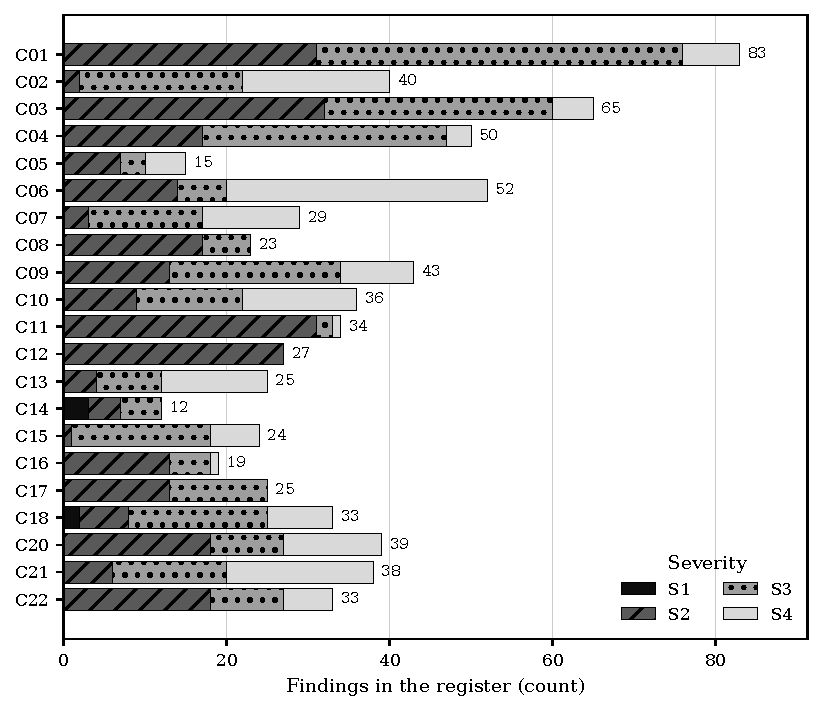
\includegraphics[width=0.9\textwidth]{results-findings}
\caption{Findings of the validation of each case with committed results, stacked by severity from critical (S1) to minor (S4), with the total at the end of each bar; the counts are read from the findings register of the product and cover all variants of a case.}
\label{fig:results-findings}
\end{figure}

By status, \rsFindOpen{} findings (\rsFindOpenShare{}\,\%) are open, \rsFindAccepted{} are risk accepted by rule and \rsFindClosed{} are closed after validation; none is overdue. The opinion level of a case follows from a stated rule on its open findings: level 1 with no open finding, level 2 with findings of severity S3 or S4 only, level 3 with any significant finding (S2) and level 4 with any critical finding (S1); an anchor of 5 to 10 percent of risk-weighted assets gives level 3 and one of 10 percent or more gives level 4, and an anchor can only raise a level. \rsLevelThreeCases{} cases are at level 3 and \rsLevelFourCases{} at level 4, and no report reaches level 1 or 2 (\rsLevelOneTwo{} reports). The rule, its deadlines and its severity scale are conventions of the product, and the opinion is the output of the rule on the evidence, not an approval or a rejection of a model. A level of 3 says that a significant finding is open; it does not say the model is unfit.

\subsection{Test lights}
\label{sec:results-lights}

\Cref{tab:results-lights} and \cref{fig:results-lights} count the tests behind the findings. Over the \rsReports{} validation reports, \rsLightsTotal{} tests end \rsLightsGreen{} green (\rsLightsGreenShare{}\,\%), \rsLightsAmber{} amber (\rsLightsAmberShare{}\,\%), \rsLightsRed{} red (\rsLightsRedShare{}\,\%) and \rsLightsNotEval{} not evaluated. The share of red varies from \rsRedLowShare{}\,\% in \rsRedLowCase{} to \rsRedHighShare{}\,\% in \rsRedHighCase{}, and \rsRedZeroCount{} cases (\rsRedZeroCases{}) have no red test. A red light is not a conclusion about a model: it depends on the size of the test, and C22 shows that two tests of the battery, the Jeffreys test and the normal test over five years, and two common settings, the Hosmer--Lemeshow test on a validation sample and the population stability index in small samples, reject a correct model more often than their level, so some of the red lights of the long batteries are the property of the instrument. The reading of a light with the measured error rates of its test is the subject of the validation section, and a case with many tests and a high red share shows a long battery meeting a hard question, not necessarily a worse model.

\begin{figure}[htbp]
\centering
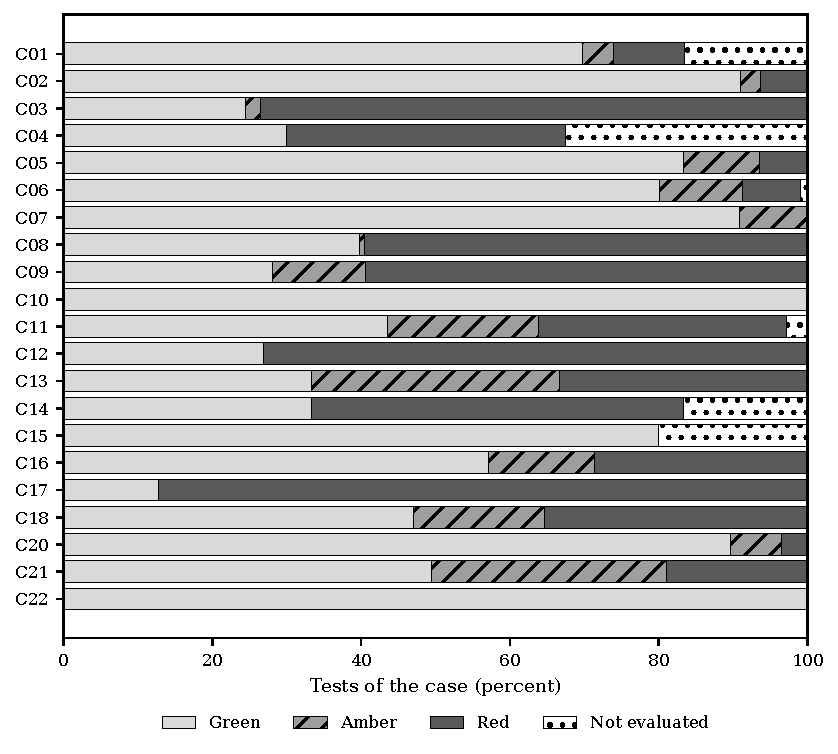
\includegraphics[width=0.9\textwidth]{results-lights}
\caption{Share of the tests of each case that end green, amber, red or not evaluated, summed over the validation reports of the case; the bars add to one hundred percent, and a case with no red test shows no red segment.}
\label{fig:results-lights}
\end{figure}

{\footnotesize
\setlength{\tabcolsep}{3pt}
\renewcommand{\arraystretch}{1.12}
\begin{longtable}{lrrrrrrr}
\caption{Test lights in the validation reports of each case, summed over the reports of the case (one report for each model fit or default variant): the number of reports, their opinion level, the tests that end green, amber, red and not evaluated, and the share of red among all tests of the case.}\label{tab:results-lights}\\
\toprule
Case & Reports & Op. & Green & Amber & Red & Not evaluated & Red (\%) \\
\midrule
\endfirsthead
\toprule
Case & Reports & Op. & Green & Amber & Red & Not evaluated & Red (\%) \\
\midrule
\endhead
\bottomrule
\endfoot
C01 & 3 & 3 & 375 & 23 & 51 & 89 & 9.5 \\
C02 & 1 & 3 & 101 & 3 & 7 & 0 & 6.3 \\
C03 & 1 & 3 & 12 & 1 & 36 & 0 & 73.5 \\
C04 & 1 & 3 & 24 & 0 & 30 & 26 & 37.5 \\
C05 & 2 & 3 & 155 & 19 & 12 & 0 & 6.5 \\
C06 & 6 & 3 & 173 & 24 & 17 & 2 & 7.9 \\
C07 & 1 & 3 & 10 & 1 & 0 & 0 & 0.0 \\
C08 & 6 & 3 & 62 & 1 & 93 & 0 & 59.6 \\
C09 & 1 & 3 & 9 & 4 & 19 & 0 & 59.4 \\
C10 & 1 & 3 & 15 & 0 & 0 & 0 & 0.0 \\
C11 & 1 & 3 & 94 & 44 & 72 & 6 & 33.3 \\
C12 & 1 & 3 & 11 & 0 & 30 & 0 & 73.2 \\
C13 & 1 & 3 & 1 & 1 & 1 & 0 & 33.3 \\
C14 & 1 & 4 & 2 & 0 & 3 & 1 & 50.0 \\
C15 & 1 & 3 & 4 & 0 & 0 & 1 & 0.0 \\
C16 & 1 & 3 & 4 & 1 & 2 & 0 & 28.6 \\
C17 & 1 & 3 & 6 & 0 & 41 & 0 & 87.2 \\
C18 & 1 & 4 & 8 & 3 & 6 & 0 & 35.3 \\
C20 & 1 & 3 & 26 & 2 & 1 & 0 & 3.4 \\
C21 & 1 & 3 & 47 & 30 & 18 & 0 & 18.9 \\
C22 & 1 & 3 & 5 & 0 & 0 & 0 & 0.0 \\
\end{longtable}
}


\subsection{The proposed methods}
\label{sec:results-proposed-summary}

The seven methods that Contraste proposes were evaluated against criteria fixed before their evaluation, and they did not all succeed. The test of a behavioural assumption changed at a limit breach flags \pxPpEightStatedAlt{} of the histories with a change at a breach date and \pxPpEightStatedNull{} of those with unrelated changes on a stated parameter, as $1-(1-\lambda)^{m}$ predicts; on a parameter re-estimated at each date, as in case C14, it flags \pxPpEightFitNull{} of null banks and ranks a lengthening of two years at an ROC area of \pxPpEightFitAuc{}, and a tolerance calibrated at 5\,\% holds \pxPpEightTolNull{} false flags but detects \pxPpEightTolTwo{} of the two-year lengthenings, so \pxPpEightRefuted{} of its predictions failed (\cref{sec:bs8}). The corrections of three validation tests remove the error each targets at a cost in power: with equal calibration and test windows the binomial coverage test rejects an exchangeable window in \pxPpTenBinomEqual{} of the replications against \pxPpTenBetaBin{} for the Beta-Binomial test; a fixed drop of 0.05 raises a false alarm in \pxPpTenFixedFive{} of shift-free replications against \pxPpTenPerm{} for the permutation reference, which detects a shift of two standard deviations in \pxPpTenPermPower{} against \pxPpTenFixedPower{}; and the cut 0.20 of the situation test raises a false alarm in \pxPpTenCutTwenty{} of null replications with 400 applicants against \pxPpTenCutTen{} for the cut 0.10 but detects a gap of 0.2 in \pxPpTenPowTwentyGapTwo{} against \pxPpTenPowTenGapTwo{}, and \pxPpTenHypRefuted{} of its \pxPpTenHypTotal{} predictions are refuted, all about that cut (\cref{sec:bs10}). The reverse liquidity stress returns a multiplier of \pxPpElevenAdv{} on the adverse base and \pxPpElevenExt{} on the extreme base for a target of 30 days, agrees with an independent oracle on every outcome of \pxPpElevenInst{} seeded instances and refuses the fast-run base; scored against the labelled run of March 2023, the base calibrated on the rows before 2023 models \pxPpElevenSvbModel{} of the deposits in the two days against the 0.85 reported (a ratio of \pxPpElevenSvbRatio{}), and the multiplier that reproduces the run is \pxPpElevenSvbMult{} times the calibrated rate, so the rule runs as specified and the base does not reproduce the run (\cref{sec:bs11}). The scale-and-level complement to the attribution test flags the stale-volatility model, as the union of its three statistics at a family size of \pxThirteenSize{}\,\%, in \pxThirteenUnionPower{}\,\% of \pxThirteenN{} replications at a held-out false-flag rate of \pxThirteenNullUnion{}\,\%, where the regulatory zone flags it in \pxThirteenPla{}\,\%, and its criterion of \pxThirteenThresholdPower{}\,\% holds (\cref{sec:bs13}). The anchored tipping-point probability covers the true probability in \pxFourteenAnchoredNine{}\,\% of \pxFourteenReps{} repetitions at an informativeness of 9, but the clause on the existing treatments fails, since in the first-year cohort the industry and unfollowed treatments cover \pxFourteenIndustryNine{}\,\% of the repetitions, and its stability criterion of \pxFourteenStability{}\,\% fails on the agency's cohorts (\pxFourteenCccShare{}\,\% for the lowest grade), so its stability clause fails too, and Manski's band covers as often (\cref{sec:bs14}). The e-process monitors hold their size, rejecting a correct model in \pxFifteenENull{}\,\% of series where the Kupiec rule on the trailing window rejects in \pxFifteenKupTrail{}\,\%, and detect a hit rate three times too high at day \pxFifteenXThreeDay{} on one seed, but at day \pxFifteenPoolThreeMed{} against \pxFifteenPoolLight{} for the traffic light when \pxFifteenPoolSeeds{} seeds are pooled, so the delay criterion fails at three times the nominal rate; on the pooled replication one Kupiec reading has \pxFifteenPoolCostThree{} points more power at day 250, so the power criterion fails too (\cref{sec:bs15}). The conformal recalibration meets its criterion in \pxSixteenCellsHold{} of \pxSixteenCells{} cells on the asymptotic p-values and in \pxPpSixteenHoneGain{} of them against the null of the wrapped count (\cref{sec:bs16}). The summary table of the section of the proposed methods (\cref{tab:proposed-summary}) gives a headline quantity for twelve of its sixteen contributions, as counts and point values without intervals; the other four report theirs, with intervals, in \cref{tab:proposed-pla,tab:proposed-anchored,tab:proposed-sequential,tab:proposed-conformal}.

\subsection{The methods compared, question by question}
\label{sec:results-methods-compared}
% Generated by tables/make_methods-compared.py from data/derived/benchmark/methods-compared.json; do not edit.
\newcommand{\bmNQuestions}{twelve}
\newcommand{\bmNCells}{1\,844}
\newcommand{\bmNFilled}{1\,529}
\newcommand{\bmNNull}{315}
\newcommand{\bmNLeftOut}{four}
\newcommand{\bmNNotBuilt}{two}
\newcommand{\bmCodeVersion}{1.00.001}
\newcommand{\bmSchemaVersion}{1.0.0}


The case sections above rank the methods of one case on that case's own data. This subsection puts the methods that answer one question side by side, under one protocol, as the committed document \texttt{data/derived/benchmark/methods-compared.json} holds them (contract \texttt{benchmark-methods}, \cref{sec:contract-benchmark-methods}). The document covers \bmNQuestions{} questions and \bmNCells{} cells, of which \bmNFilled{} carry a value and \bmNNull{} are null, each with the reason the product does not compute it. It recomputes nothing: every value is copied from a committed case document or manuscript result file, with its path, its JSON pointer and the SHA-256 of that file, and the document was built by version \bmCodeVersion{} of the code. A method is shown with one of four standings. Long-established and recent published methods are those the product runs from the literature, and Proposed in this work marks the methods the product itself proposes (\cref{sec:results-proposed-summary}); Reference marks a comparator that has no row in the method ladder (the product's list of methods), such as an oracle that uses information a lender never has, or a constant prediction. Within a table the best cell of each column is in bold, chosen by the rule the document declares for that metric (lower, higher, nearer a stated value, or an order of words), and a metric declared as context is never ranked. The document copies point values as the case documents hold them; it carries no interval, so a difference between two cells is a difference of point values and not a claim of significance, and the intervals sit in the case sections of the report. Each question below states its protocol, the tables, the reading the document generates from them, and then what the tables show and do not show.

% Generated by tables/make_methods-compared.py from data/derived/benchmark/methods-compared.json; do not edit.
\subsubsection{VaR and ES forecasts in stress windows}
\label{sec:results-methods-compared-q1}

This question is answered on case C11. One rolling schedule per window: every rule forecasts day t from data up to t-1 on an estimation window of 1,000 days, with its hyperparameters fixed on 1995 to 2003 and never tuned on the test window; the adaptive conformal recalibration runs on the same days. The run ``Rolling schedule, six windows'' reads as follows: Rolling forecasts on the C11 windows, 1,000-day estimation window, one document per window; its random seed is 42. Table~\ref{tab:bm-q1-methods} lists the 22 methods the document compares, eleven long-established, seven recent published, three proposed in this work and one reference, with the section of this report that describes each. Tables~\ref{tab:bm-q1-1}, \ref{tab:bm-q1-2}, \ref{tab:bm-q1-3}, \ref{tab:bm-q1-4}, \ref{tab:bm-q1-5}, \ref{tab:bm-q1-6}, \ref{tab:bm-q1-7} give the values, one table for each group of metrics that share a run and a layout.

{\footnotesize\setlength{\tabcolsep}{3pt}
% bm-table-methods Q1
\begin{longtable}{>{\raggedright\arraybackslash}p{0.38\textwidth}>{\raggedright\arraybackslash}p{0.17\textwidth}>{\raggedright\arraybackslash}p{0.27\textwidth}>{\raggedright\arraybackslash}p{0.10\textwidth}}
\caption{The methods compared on the question VaR and ES forecasts in stress windows: the standing of each method, the source and the year the document records for it, and the section of this report that describes it; a dash marks a method with no source recorded or with no section of its own.}\label{tab:bm-q1-methods}\\
\toprule Method & Standing & Source & Section \\ \midrule \endfirsthead
\toprule Method & Standing & Source & Section \\ \midrule \endhead
Age-weighted historical simulation & Long-established & Boudoukh, Richardson and Whitelaw (1998)~\citep{market:boudoukh1998} & \ref{sec:m18} \\
Cornish-Fisher on rolling moments & Long-established & Cornish and Fisher (1938)~\citep{market:cornishfisher1938} & \ref{sec:m18} \\
Delta-normal on rolling moments & Long-established & RiskMetrics Technical Document (1996)~\citep{market:riskmetrics1996} & \ref{sec:m18} \\
EGARCH with Student-t errors & Long-established & Nelson (1991)~\citep{market:nelson1991} & \ref{sec:m18} \\
Conditional extreme value theory (McNeil and Frey) & Long-established & McNeil and Frey (2000)~\citep{market:mcneilfrey2000} & \ref{sec:m18} \\
EWMA (RiskMetrics) & Long-established & RiskMetrics Technical Document (1996)~\citep{market:riskmetrics1996} & \ref{sec:m18} \\
Filtered historical simulation & Long-established & -- & \ref{sec:m18} \\
GARCH(1,1) with Student-t errors & Long-established & Bollerslev (1986)~\citep{market:bollerslev1986} & \ref{sec:m18} \\
GJR-GARCH with Student-t errors & Long-established & Glosten, Jagannathan and Runkle (1993)~\citep{market:gjr1993} & \ref{sec:m18} \\
Historical simulation, 250 days & Long-established & Pritsker (2001)~\citep{market:pritsker2001} & \ref{sec:m18} \\
Historical simulation, 500 days & Long-established & Pritsker (2001)~\citep{market:pritsker2001} & \ref{sec:m18} \\
Quantile network trained on the FZ0 loss & Recent published & -- & \ref{sec:m30} \\
CAViaR, asymmetric slope & Recent published & Engle and Manganelli (2004)~\citep{market:engleManganelli2004} & \ref{sec:m38} \\
ES-CAViaR (Taylor) & Recent published & Taylor (2019)~\citep{market:taylor2019} & \ref{sec:m38} \\
CAViaR, symmetric absolute value & Recent published & Engle and Manganelli (2004)~\citep{market:engleManganelli2004} & \ref{sec:m38} \\
GAS under the FZ0 loss, one factor & Recent published & Patton, Ziegel and Chen (2019)~\citep{market:pattonziegelchen2019} & \ref{sec:m38} \\
GAS under the FZ0 loss, two factors & Recent published & Patton, Ziegel and Chen (2019)~\citep{market:pattonziegelchen2019} & \ref{sec:m38} \\
Hybrid GARCH-FZ & Recent published & Patton, Ziegel and Chen (2019)~\citep{market:pattonziegelchen2019} & \ref{sec:m38} \\
Filtered historical simulation, with adaptive conformal recalibration & Proposed in this work & -- & \ref{sec:bs16} \\
GARCH(1,1) with Student-t errors, with adaptive conformal recalibration & Proposed in this work & -- & \ref{sec:bs16} \\
Historical simulation, 250 days, with adaptive conformal recalibration & Proposed in this work & -- & \ref{sec:bs16} \\
Expected exceedances of a correct model & Reference & -- & -- \\
\bottomrule
\end{longtable}
}

{\footnotesize\setlength{\tabcolsep}{3pt}
% bm-table Q1 normal cols=fz0_1/calm-2004-06;fz0_1/equity-2007-09;fz0_1/equity-2020;fz0_1/rates-2022;fz0_1/fx-2008;fz0_1/mixed-2023
\begin{longtable}{>{\raggedright\arraybackslash}p{0.25\textwidth}>{\raggedleft\arraybackslash}p{0.105\textwidth}>{\raggedleft\arraybackslash}p{0.105\textwidth}>{\raggedleft\arraybackslash}p{0.105\textwidth}>{\raggedleft\arraybackslash}p{0.105\textwidth}>{\raggedleft\arraybackslash}p{0.105\textwidth}>{\raggedleft\arraybackslash}p{0.105\textwidth}}
\caption{VaR and ES forecasts in stress windows: Mean FZ0 loss, 1\% level (FZ0 loss; lower is better), for each method, on the run Rolling schedule, six windows. The best value of a column by the declared rule is in bold, ties all in bold; a dash marks a cell without a value, and the notes below the table state why.}\label{tab:bm-q1-1}\\
\toprule Method & Calm 2004 to 2006 & Equities 2007 to 2009 & Equities 2020 & Rates 2022 & Currencies 2008 & Mixed 2023 \\ \midrule \endfirsthead
\toprule Method & Calm 2004 to 2006 & Equities 2007 to 2009 & Equities 2020 & Rates 2022 & Currencies 2008 & Mixed 2023 \\ \midrule \endhead
\multicolumn{7}{l}{\emph{Long-established}} \\
Age-weighted historical simulation & $-$4.491 & $-$2.733 & $-$0.388 & $-$3.597 & $-$3.386 & $-$4.070 \\ % bm-row awhs
Cornish-Fisher on rolling moments & -- & -- & -- & -- & -- & -- \\ % bm-row cf-rolling
Delta-normal on rolling moments & $-$4.378 & 2.037 & 13.29 & $-$3.005 & $-$0.881 & $-$4.040 \\ % bm-row dn-rolling
EGARCH with Student-t errors & $-$4.504 & $-$2.522 & $-$1.451 & $-$3.640 & $-$3.453 & $-$4.358 \\ % bm-row egarch-t
Conditional extreme value theory (McNeil and Frey) & $-$4.473 & $-$2.826 & $-$1.928 & $-$3.666 & $-$3.510 & $-$4.260 \\ % bm-row evt-mf
EWMA (RiskMetrics) & $-$4.498 & $-$2.676 & 1.004 & \textbf{$-$3.811} & $-$3.488 & $-$4.289 \\ % bm-row ewma
Filtered historical simulation & $-$4.460 & $-$2.797 & \textbf{$-$1.986} & $-$3.692 & $-$3.516 & $-$4.225 \\ % bm-row fhs
GARCH(1,1) with Student-t errors & $-$4.490 & $-$2.778 & $-$1.642 & $-$3.664 & $-$3.493 & $-$4.420 \\ % bm-row garch-t
GJR-GARCH with Student-t errors & \textbf{$-$4.521} & $-$2.876 & $-$1.313 & $-$3.558 & $-$3.503 & $-$4.439 \\ % bm-row gjr-t
Historical simulation, 250 days & $-$4.470 & $-$2.364 & 1.053 & $-$3.462 & $-$3.178 & $-$3.797 \\ % bm-row hs-250
Historical simulation, 500 days & $-$4.471 & $-$1.966 & 1.896 & $-$3.621 & $-$2.823 & $-$3.957 \\ % bm-row hs-500
\multicolumn{7}{l}{\emph{Recent published}} \\
Quantile network trained on the FZ0 loss & $-$4.286 & $-$2.371 & $-$1.669 & $-$3.445 & $-$3.527 & $-$4.134 \\ % bm-row nn-fz
CAViaR, asymmetric slope & -- & -- & -- & -- & -- & -- \\ % bm-row caviar-as
ES-CAViaR (Taylor) & $-$4.472 & $-$2.747 & $-$1.864 & $-$3.646 & \textbf{$-$3.557} & $-$4.197 \\ % bm-row caviar-es
CAViaR, symmetric absolute value & -- & -- & -- & -- & -- & -- \\ % bm-row caviar-sav
GAS under the FZ0 loss, one factor & $-$4.448 & $-$2.042 & $-$0.288 & $-$3.226 & 11.91 & $-$4.113 \\ % bm-row gas-fz-1
GAS under the FZ0 loss, two factors & $-$4.436 & $-$2.236 & $-$0.085 & $-$3.282 & 1.555 & $-$4.059 \\ % bm-row gas-fz-2
Hybrid GARCH-FZ & $-$4.435 & $-$1.802 & $-$0.859 & $-$3.294 & 8.701 & $-$4.193 \\ % bm-row gas-hybrid
\multicolumn{7}{l}{\emph{Proposed in this work}} \\
Filtered historical simulation, with adaptive conformal recalibration & $-$4.461 & $-$2.886 & $-$1.917 & $-$3.659 & $-$3.508 & $-$4.254 \\ % bm-row fhs-aci
GARCH(1,1) with Student-t errors, with adaptive conformal recalibration & $-$4.457 & \textbf{$-$2.894} & $-$1.593 & $-$3.671 & $-$3.479 & \textbf{$-$4.455} \\ % bm-row garch-t-aci
Historical simulation, 250 days, with adaptive conformal recalibration & $-$4.432 & $-$2.771 & $-$0.724 & $-$3.664 & $-$3.457 & $-$3.839 \\ % bm-row hs-250-aci
\bottomrule
\end{longtable}
}

A dash in Table~\ref{tab:bm-q1-1} is a cell the product does not compute, for the stated reason: the rule forecasts no expected shortfall, so its FZ0 loss is undefined (Cornish-Fisher on rolling moments, CAViaR, asymmetric slope and CAViaR, symmetric absolute value).

{\footnotesize\setlength{\tabcolsep}{3pt}
% bm-table Q1 normal cols=fz0_25/calm-2004-06;fz0_25/equity-2007-09;fz0_25/equity-2020;fz0_25/rates-2022;fz0_25/fx-2008;fz0_25/mixed-2023
\begin{longtable}{>{\raggedright\arraybackslash}p{0.25\textwidth}>{\raggedleft\arraybackslash}p{0.105\textwidth}>{\raggedleft\arraybackslash}p{0.105\textwidth}>{\raggedleft\arraybackslash}p{0.105\textwidth}>{\raggedleft\arraybackslash}p{0.105\textwidth}>{\raggedleft\arraybackslash}p{0.105\textwidth}>{\raggedleft\arraybackslash}p{0.105\textwidth}}
\caption{VaR and ES forecasts in stress windows: Mean FZ0 loss, 2.5\% level (FZ0 loss; lower is better), for each method, on the run Rolling schedule, six windows. The best value of a column by the declared rule is in bold, ties all in bold; a dash marks a cell without a value, and the notes below the table state why.}\label{tab:bm-q1-2}\\
\toprule Method & Calm 2004 to 2006 & Equities 2007 to 2009 & Equities 2020 & Rates 2022 & Currencies 2008 & Mixed 2023 \\ \midrule \endfirsthead
\toprule Method & Calm 2004 to 2006 & Equities 2007 to 2009 & Equities 2020 & Rates 2022 & Currencies 2008 & Mixed 2023 \\ \midrule \endhead
\multicolumn{7}{l}{\emph{Long-established}} \\
Age-weighted historical simulation & $-$4.653 & $-$2.908 & $-$1.108 & $-$3.931 & $-$3.592 & $-$4.252 \\ % bm-row awhs
Cornish-Fisher on rolling moments & -- & -- & -- & -- & -- & -- \\ % bm-row cf-rolling
Delta-normal on rolling moments & $-$4.531 & $-$0.478 & 5.010 & $-$3.548 & $-$2.215 & $-$4.207 \\ % bm-row dn-rolling
EGARCH with Student-t errors & $-$4.651 & $-$2.744 & $-$2.129 & $-$3.893 & $-$3.682 & $-$4.593 \\ % bm-row egarch-t
Conditional extreme value theory (McNeil and Frey) & $-$4.637 & $-$2.920 & $-$2.364 & $-$3.926 & \textbf{$-$3.716} & $-$4.523 \\ % bm-row evt-mf
EWMA (RiskMetrics) & \textbf{$-$4.659} & $-$2.890 & $-$0.803 & \textbf{$-$4.002} & $-$3.707 & $-$4.454 \\ % bm-row ewma
Filtered historical simulation & $-$4.642 & $-$2.957 & $-$2.344 & $-$3.932 & $-$3.712 & $-$4.540 \\ % bm-row fhs
GARCH(1,1) with Student-t errors & $-$4.648 & $-$2.887 & $-$2.175 & $-$3.906 & $-$3.706 & $-$4.612 \\ % bm-row garch-t
GJR-GARCH with Student-t errors & $-$4.659 & $-$2.941 & $-$2.110 & $-$3.799 & $-$3.703 & \textbf{$-$4.623} \\ % bm-row gjr-t
Historical simulation, 250 days & $-$4.621 & $-$2.596 & $-$0.195 & $-$3.794 & $-$3.429 & $-$4.094 \\ % bm-row hs-250
Historical simulation, 500 days & $-$4.645 & $-$2.235 & 0.246 & $-$3.779 & $-$3.010 & $-$4.197 \\ % bm-row hs-500
\multicolumn{7}{l}{\emph{Recent published}} \\
Quantile network trained on the FZ0 loss & $-$4.588 & $-$2.856 & \textbf{$-$2.368} & $-$3.909 & $-$3.685 & $-$4.374 \\ % bm-row nn-fz
CAViaR, asymmetric slope & -- & -- & -- & -- & -- & -- \\ % bm-row caviar-as
ES-CAViaR (Taylor) & $-$4.632 & $-$2.869 & $-$2.236 & $-$3.824 & $-$3.709 & $-$4.444 \\ % bm-row caviar-es
CAViaR, symmetric absolute value & -- & -- & -- & -- & -- & -- \\ % bm-row caviar-sav
GAS under the FZ0 loss, one factor & $-$4.630 & $-$2.966 & $-$1.594 & $-$3.799 & $-$3.638 & $-$4.457 \\ % bm-row gas-fz-1
GAS under the FZ0 loss, two factors & $-$4.611 & $-$2.672 & $-$1.383 & $-$3.798 & $-$3.276 & $-$4.424 \\ % bm-row gas-fz-2
Hybrid GARCH-FZ & $-$4.603 & $-$2.851 & $-$1.550 & $-$3.811 & $-$2.542 & $-$4.469 \\ % bm-row gas-hybrid
\multicolumn{7}{l}{\emph{Proposed in this work}} \\
Filtered historical simulation, with adaptive conformal recalibration & $-$4.635 & \textbf{$-$3.007} & $-$2.309 & $-$3.942 & $-$3.709 & $-$4.553 \\ % bm-row fhs-aci
GARCH(1,1) with Student-t errors, with adaptive conformal recalibration & $-$4.634 & $-$2.992 & $-$2.222 & $-$3.920 & $-$3.707 & $-$4.605 \\ % bm-row garch-t-aci
Historical simulation, 250 days, with adaptive conformal recalibration & $-$4.622 & $-$2.967 & $-$1.427 & $-$3.919 & $-$3.576 & $-$4.111 \\ % bm-row hs-250-aci
\bottomrule
\end{longtable}
}

A dash in Table~\ref{tab:bm-q1-2} is a cell the product does not compute, for the stated reason: the rule forecasts no expected shortfall, so its FZ0 loss is undefined (Cornish-Fisher on rolling moments, CAViaR, asymmetric slope and CAViaR, symmetric absolute value).

{\footnotesize\setlength{\tabcolsep}{3pt}
% bm-table Q1 normal cols=exceed_1/calm-2004-06;exceed_1/equity-2007-09;exceed_1/equity-2020;exceed_1/rates-2022;exceed_1/fx-2008;exceed_1/mixed-2023
\begin{longtable}{>{\raggedright\arraybackslash}p{0.25\textwidth}>{\raggedleft\arraybackslash}p{0.105\textwidth}>{\raggedleft\arraybackslash}p{0.105\textwidth}>{\raggedleft\arraybackslash}p{0.105\textwidth}>{\raggedleft\arraybackslash}p{0.105\textwidth}>{\raggedleft\arraybackslash}p{0.105\textwidth}>{\raggedleft\arraybackslash}p{0.105\textwidth}}
\caption{VaR and ES forecasts in stress windows: Exceedances, 1\% level (days; nearer the expected exceedances, 1\% level is better), for each method, on the run Rolling schedule, six windows. The best value of a column by the declared rule is in bold, ties all in bold; a dash marks a cell without a value, and the notes below the table state why.}\label{tab:bm-q1-3}\\
\toprule Method & Calm 2004 to 2006 & Equities 2007 to 2009 & Equities 2020 & Rates 2022 & Currencies 2008 & Mixed 2023 \\ \midrule \endfirsthead
\toprule Method & Calm 2004 to 2006 & Equities 2007 to 2009 & Equities 2020 & Rates 2022 & Currencies 2008 & Mixed 2023 \\ \midrule \endhead
\multicolumn{7}{l}{\emph{Long-established}} \\
Age-weighted historical simulation & 10 & 16 & 5 & 7 & 6 & 0 \\ % bm-row awhs
Cornish-Fisher on rolling moments & 1 & 26 & 8 & \textbf{4} & 14 & 0 \\ % bm-row cf-rolling
Delta-normal on rolling moments & 0 & 57 & 16 & 15 & 23 & 0 \\ % bm-row dn-rolling
EGARCH with Student-t errors & 10 & 20 & 3 & 6 & \textbf{3} & 0 \\ % bm-row egarch-t
Conditional extreme value theory (McNeil and Frey) & \textbf{8} & 13 & \textbf{2} & 5 & \textbf{3} & 0 \\ % bm-row evt-mf
EWMA (RiskMetrics) & 10 & 16 & 7 & 6 & \textbf{3} & 0 \\ % bm-row ewma
Filtered historical simulation & \textbf{8} & 13 & \textbf{2} & 5 & \textbf{3} & 0 \\ % bm-row fhs
GARCH(1,1) with Student-t errors & 9 & 16 & 3 & 6 & \textbf{3} & 0 \\ % bm-row garch-t
GJR-GARCH with Student-t errors & 9 & 14 & 3 & 6 & \textbf{3} & 0 \\ % bm-row gjr-t
Historical simulation, 250 days & 9 & 19 & 8 & 8 & 10 & 0 \\ % bm-row hs-250
Historical simulation, 500 days & 3 & 27 & 10 & 8 & 13 & 0 \\ % bm-row hs-500
\multicolumn{7}{l}{\emph{Recent published}} \\
Quantile network trained on the FZ0 loss & 22 & 16 & 4 & 11 & 5 & \textbf{1} \\ % bm-row nn-fz
CAViaR, asymmetric slope & 5 & 15 & 4 & 6 & 4 & 0 \\ % bm-row caviar-as
ES-CAViaR (Taylor) & 4 & 13 & 4 & 6 & 5 & 0 \\ % bm-row caviar-es
CAViaR, symmetric absolute value & 4 & 13 & 4 & 6 & 5 & 0 \\ % bm-row caviar-sav
GAS under the FZ0 loss, one factor & 4 & 20 & 6 & 10 & 11 & 0 \\ % bm-row gas-fz-1
GAS under the FZ0 loss, two factors & 3 & 26 & 7 & 8 & 19 & 0 \\ % bm-row gas-fz-2
Hybrid GARCH-FZ & 3 & 27 & 6 & 9 & 16 & 0 \\ % bm-row gas-hybrid
\multicolumn{7}{l}{\emph{Proposed in this work}} \\
Filtered historical simulation, with adaptive conformal recalibration & \textbf{8} & 7 & \textbf{2} & 5 & 2 & 0 \\ % bm-row fhs-aci
GARCH(1,1) with Student-t errors, with adaptive conformal recalibration & \textbf{8} & \textbf{6} & \textbf{2} & \textbf{4} & 2 & 0 \\ % bm-row garch-t-aci
Historical simulation, 250 days, with adaptive conformal recalibration & \textbf{8} & 11 & 6 & \textbf{4} & 5 & 0 \\ % bm-row hs-250-aci
\bottomrule
\end{longtable}
}

{\footnotesize\setlength{\tabcolsep}{3pt}
% bm-table Q1 normal cols=expected_1/calm-2004-06;expected_1/equity-2007-09;expected_1/equity-2020;expected_1/rates-2022;expected_1/fx-2008;expected_1/mixed-2023
\begin{longtable}{>{\raggedright\arraybackslash}p{0.25\textwidth}>{\raggedleft\arraybackslash}p{0.105\textwidth}>{\raggedleft\arraybackslash}p{0.105\textwidth}>{\raggedleft\arraybackslash}p{0.105\textwidth}>{\raggedleft\arraybackslash}p{0.105\textwidth}>{\raggedleft\arraybackslash}p{0.105\textwidth}>{\raggedleft\arraybackslash}p{0.105\textwidth}}
\caption{VaR and ES forecasts in stress windows: Expected exceedances, 1\% level (days; context, not ranked), for each method, on the run Rolling schedule, six windows. The best value of a column by the declared rule is in bold, ties all in bold; a dash marks a cell without a value, and the notes below the table state why.}\label{tab:bm-q1-4}\\
\toprule Method & Calm 2004 to 2006 & Equities 2007 to 2009 & Equities 2020 & Rates 2022 & Currencies 2008 & Mixed 2023 \\ \midrule \endfirsthead
\toprule Method & Calm 2004 to 2006 & Equities 2007 to 2009 & Equities 2020 & Rates 2022 & Currencies 2008 & Mixed 2023 \\ \midrule \endhead
\multicolumn{7}{l}{\emph{Reference}} \\
Expected exceedances of a correct model & 7.500 & 5.040 & 1.040 & 2.490 & 2.510 & 0.640 \\ % bm-row expected
\bottomrule
\end{longtable}
}

{\footnotesize\setlength{\tabcolsep}{3pt}
% bm-table Q1 normal cols=zone_1/calm-2004-06;zone_1/equity-2007-09;zone_1/equity-2020;zone_1/rates-2022;zone_1/fx-2008;zone_1/mixed-2023
\begin{longtable}{>{\raggedright\arraybackslash}p{0.25\textwidth}>{\raggedleft\arraybackslash}p{0.105\textwidth}>{\raggedleft\arraybackslash}p{0.105\textwidth}>{\raggedleft\arraybackslash}p{0.105\textwidth}>{\raggedleft\arraybackslash}p{0.105\textwidth}>{\raggedleft\arraybackslash}p{0.105\textwidth}>{\raggedleft\arraybackslash}p{0.105\textwidth}}
\caption{VaR and ES forecasts in stress windows: Basel zone of the last 250 days, 1\% level (zone; green is best, then amber, then red), for each method, on the run Rolling schedule, six windows. The best value of a column by the declared rule is in bold, ties all in bold; a dash marks a cell without a value, and the notes below the table state why.}\label{tab:bm-q1-5}\\
\toprule Method & Calm 2004 to 2006 & Equities 2007 to 2009 & Equities 2020 & Rates 2022 & Currencies 2008 & Mixed 2023 \\ \midrule \endfirsthead
\toprule Method & Calm 2004 to 2006 & Equities 2007 to 2009 & Equities 2020 & Rates 2022 & Currencies 2008 & Mixed 2023 \\ \midrule \endhead
\multicolumn{7}{l}{\emph{Long-established}} \\
Age-weighted historical simulation & \textbf{green} & amber & not evaluated & not evaluated & amber & not evaluated \\ % bm-row awhs
Cornish-Fisher on rolling moments & \textbf{green} & red & not evaluated & not evaluated & red & not evaluated \\ % bm-row cf-rolling
Delta-normal on rolling moments & \textbf{green} & red & not evaluated & not evaluated & red & not evaluated \\ % bm-row dn-rolling
EGARCH with Student-t errors & amber & amber & not evaluated & not evaluated & \textbf{green} & not evaluated \\ % bm-row egarch-t
Conditional extreme value theory (McNeil and Frey) & \textbf{green} & \textbf{green} & not evaluated & not evaluated & \textbf{green} & not evaluated \\ % bm-row evt-mf
EWMA (RiskMetrics) & \textbf{green} & amber & not evaluated & not evaluated & \textbf{green} & not evaluated \\ % bm-row ewma
Filtered historical simulation & \textbf{green} & \textbf{green} & not evaluated & not evaluated & \textbf{green} & not evaluated \\ % bm-row fhs
GARCH(1,1) with Student-t errors & \textbf{green} & amber & not evaluated & not evaluated & \textbf{green} & not evaluated \\ % bm-row garch-t
GJR-GARCH with Student-t errors & \textbf{green} & \textbf{green} & not evaluated & not evaluated & \textbf{green} & not evaluated \\ % bm-row gjr-t
Historical simulation, 250 days & \textbf{green} & red & not evaluated & not evaluated & red & not evaluated \\ % bm-row hs-250
Historical simulation, 500 days & \textbf{green} & red & not evaluated & not evaluated & red & not evaluated \\ % bm-row hs-500
\multicolumn{7}{l}{\emph{Recent published}} \\
Quantile network trained on the FZ0 loss & amber & amber & not evaluated & not evaluated & amber & not evaluated \\ % bm-row nn-fz
CAViaR, asymmetric slope & \textbf{green} & \textbf{green} & not evaluated & not evaluated & \textbf{green} & not evaluated \\ % bm-row caviar-as
ES-CAViaR (Taylor) & \textbf{green} & \textbf{green} & not evaluated & not evaluated & amber & not evaluated \\ % bm-row caviar-es
CAViaR, symmetric absolute value & \textbf{green} & \textbf{green} & not evaluated & not evaluated & amber & not evaluated \\ % bm-row caviar-sav
GAS under the FZ0 loss, one factor & \textbf{green} & amber & not evaluated & not evaluated & red & not evaluated \\ % bm-row gas-fz-1
GAS under the FZ0 loss, two factors & \textbf{green} & red & not evaluated & not evaluated & red & not evaluated \\ % bm-row gas-fz-2
Hybrid GARCH-FZ & \textbf{green} & red & not evaluated & not evaluated & red & not evaluated \\ % bm-row gas-hybrid
\multicolumn{7}{l}{\emph{Proposed in this work}} \\
Filtered historical simulation, with adaptive conformal recalibration & -- & -- & -- & -- & -- & -- \\ % bm-row fhs-aci
GARCH(1,1) with Student-t errors, with adaptive conformal recalibration & -- & -- & -- & -- & -- & -- \\ % bm-row garch-t-aci
Historical simulation, 250 days, with adaptive conformal recalibration & -- & -- & -- & -- & -- & -- \\ % bm-row hs-250-aci
\bottomrule
\end{longtable}
}

A dash in Table~\ref{tab:bm-q1-5} is a cell the product does not compute, for the stated reason: the conformal block carries no Basel zone (Filtered historical simulation, with adaptive conformal recalibration, GARCH(1,1) with Student-t errors, with adaptive conformal recalibration and Historical simulation, 250 days, with adaptive conformal recalibration).

{\footnotesize\setlength{\tabcolsep}{3pt}
% bm-table Q1 normal cols=kupiec_1/calm-2004-06;kupiec_1/equity-2007-09;kupiec_1/equity-2020;kupiec_1/rates-2022;kupiec_1/fx-2008;kupiec_1/mixed-2023
\begin{longtable}{>{\raggedright\arraybackslash}p{0.25\textwidth}>{\raggedleft\arraybackslash}p{0.105\textwidth}>{\raggedleft\arraybackslash}p{0.105\textwidth}>{\raggedleft\arraybackslash}p{0.105\textwidth}>{\raggedleft\arraybackslash}p{0.105\textwidth}>{\raggedleft\arraybackslash}p{0.105\textwidth}>{\raggedleft\arraybackslash}p{0.105\textwidth}}
\caption{VaR and ES forecasts in stress windows: Kupiec p-value, 1\% level (p-value; higher is better), for each method, on the run Rolling schedule, six windows. The best value of a column by the declared rule is in bold, ties all in bold; a dash marks a cell without a value, and the notes below the table state why.}\label{tab:bm-q1-6}\\
\toprule Method & Calm 2004 to 2006 & Equities 2007 to 2009 & Equities 2020 & Rates 2022 & Currencies 2008 & Mixed 2023 \\ \midrule \endfirsthead
\toprule Method & Calm 2004 to 2006 & Equities 2007 to 2009 & Equities 2020 & Rates 2022 & Currencies 2008 & Mixed 2023 \\ \midrule \endhead
\multicolumn{7}{l}{\emph{Long-established}} \\
Age-weighted historical simulation & -- & -- & -- & -- & -- & -- \\ % bm-row awhs
Cornish-Fisher on rolling moments & -- & -- & -- & -- & -- & -- \\ % bm-row cf-rolling
Delta-normal on rolling moments & -- & -- & -- & -- & -- & -- \\ % bm-row dn-rolling
EGARCH with Student-t errors & -- & -- & -- & -- & -- & -- \\ % bm-row egarch-t
Conditional extreme value theory (McNeil and Frey) & -- & -- & -- & -- & -- & -- \\ % bm-row evt-mf
EWMA (RiskMetrics) & -- & -- & -- & -- & -- & -- \\ % bm-row ewma
Filtered historical simulation & \textbf{0.856} & 0.0029 & \textbf{0.401} & 0.160 & \textbf{0.763} & \textbf{0.257} \\ % bm-row fhs
GARCH(1,1) with Student-t errors & 0.594 & \ensuremath{9.2\times10^{-5}} & 0.116 & 0.058 & \textbf{0.763} & \textbf{0.257} \\ % bm-row garch-t
GJR-GARCH with Student-t errors & -- & -- & -- & -- & -- & -- \\ % bm-row gjr-t
Historical simulation, 250 days & 0.594 & \ensuremath{1.7\times10^{-6}} & \ensuremath{1.2\times10^{-5}} & 0.0053 & \ensuremath{3.3\times10^{-4}} & \textbf{0.257} \\ % bm-row hs-250
Historical simulation, 500 days & -- & -- & -- & -- & -- & -- \\ % bm-row hs-500
\multicolumn{7}{l}{\emph{Recent published}} \\
Quantile network trained on the FZ0 loss & -- & -- & -- & -- & -- & -- \\ % bm-row nn-fz
CAViaR, asymmetric slope & -- & -- & -- & -- & -- & -- \\ % bm-row caviar-as
ES-CAViaR (Taylor) & -- & -- & -- & -- & -- & -- \\ % bm-row caviar-es
CAViaR, symmetric absolute value & -- & -- & -- & -- & -- & -- \\ % bm-row caviar-sav
GAS under the FZ0 loss, one factor & -- & -- & -- & -- & -- & -- \\ % bm-row gas-fz-1
GAS under the FZ0 loss, two factors & -- & -- & -- & -- & -- & -- \\ % bm-row gas-fz-2
Hybrid GARCH-FZ & -- & -- & -- & -- & -- & -- \\ % bm-row gas-hybrid
\multicolumn{7}{l}{\emph{Proposed in this work}} \\
Filtered historical simulation, with adaptive conformal recalibration & \textbf{0.856} & 0.407 & \textbf{0.401} & 0.160 & 0.737 & \textbf{0.257} \\ % bm-row fhs-aci
GARCH(1,1) with Student-t errors, with adaptive conformal recalibration & \textbf{0.856} & \textbf{0.677} & \textbf{0.401} & \textbf{0.377} & 0.737 & \textbf{0.257} \\ % bm-row garch-t-aci
Historical simulation, 250 days, with adaptive conformal recalibration & \textbf{0.856} & 0.021 & \ensuremath{7.5\times10^{-4}} & \textbf{0.377} & 0.164 & \textbf{0.257} \\ % bm-row hs-250-aci
\bottomrule
\end{longtable}
}

A dash in Table~\ref{tab:bm-q1-6} is a cell the product does not compute, for the stated reason: not computed yet: only the three models wrapped by adaptive conformal recalibration carry a Kupiec and a conditional-coverage p-value; the other rules carry no value in the committed documents (15 methods).

{\footnotesize\setlength{\tabcolsep}{3pt}
% bm-table Q1 normal cols=cc_1/calm-2004-06;cc_1/equity-2007-09;cc_1/equity-2020;cc_1/rates-2022;cc_1/fx-2008;cc_1/mixed-2023
\begin{longtable}{>{\raggedright\arraybackslash}p{0.25\textwidth}>{\raggedleft\arraybackslash}p{0.105\textwidth}>{\raggedleft\arraybackslash}p{0.105\textwidth}>{\raggedleft\arraybackslash}p{0.105\textwidth}>{\raggedleft\arraybackslash}p{0.105\textwidth}>{\raggedleft\arraybackslash}p{0.105\textwidth}>{\raggedleft\arraybackslash}p{0.105\textwidth}}
\caption{VaR and ES forecasts in stress windows: Conditional-coverage p-value, 1\% level (p-value; higher is better), for each method, on the run Rolling schedule, six windows. The best value of a column by the declared rule is in bold, ties all in bold; a dash marks a cell without a value, and the notes below the table state why.}\label{tab:bm-q1-7}\\
\toprule Method & Calm 2004 to 2006 & Equities 2007 to 2009 & Equities 2020 & Rates 2022 & Currencies 2008 & Mixed 2023 \\ \midrule \endfirsthead
\toprule Method & Calm 2004 to 2006 & Equities 2007 to 2009 & Equities 2020 & Rates 2022 & Currencies 2008 & Mixed 2023 \\ \midrule \endhead
\multicolumn{7}{l}{\emph{Long-established}} \\
Age-weighted historical simulation & -- & -- & -- & -- & -- & -- \\ % bm-row awhs
Cornish-Fisher on rolling moments & -- & -- & -- & -- & -- & -- \\ % bm-row cf-rolling
Delta-normal on rolling moments & -- & -- & -- & -- & -- & -- \\ % bm-row dn-rolling
EGARCH with Student-t errors & -- & -- & -- & -- & -- & -- \\ % bm-row egarch-t
Conditional extreme value theory (McNeil and Frey) & -- & -- & -- & -- & -- & -- \\ % bm-row evt-mf
EWMA (RiskMetrics) & -- & -- & -- & -- & -- & -- \\ % bm-row ewma
Filtered historical simulation & \textbf{0.902} & 0.0085 & \textbf{0.676} & 0.343 & 0.921 & -- \\ % bm-row fhs
GARCH(1,1) with Student-t errors & 0.777 & \ensuremath{2.8\times10^{-4}} & 0.265 & 0.147 & 0.921 & -- \\ % bm-row garch-t
GJR-GARCH with Student-t errors & -- & -- & -- & -- & -- & -- \\ % bm-row gjr-t
Historical simulation, 250 days & 0.777 & \ensuremath{5.0\times10^{-6}} & \ensuremath{1.9\times10^{-5}} & 0.016 & 0.0011 & -- \\ % bm-row hs-250
Historical simulation, 500 days & -- & -- & -- & -- & -- & -- \\ % bm-row hs-500
\multicolumn{7}{l}{\emph{Recent published}} \\
Quantile network trained on the FZ0 loss & -- & -- & -- & -- & -- & -- \\ % bm-row nn-fz
CAViaR, asymmetric slope & -- & -- & -- & -- & -- & -- \\ % bm-row caviar-as
ES-CAViaR (Taylor) & -- & -- & -- & -- & -- & -- \\ % bm-row caviar-es
CAViaR, symmetric absolute value & -- & -- & -- & -- & -- & -- \\ % bm-row caviar-sav
GAS under the FZ0 loss, one factor & -- & -- & -- & -- & -- & -- \\ % bm-row gas-fz-1
GAS under the FZ0 loss, two factors & -- & -- & -- & -- & -- & -- \\ % bm-row gas-fz-2
Hybrid GARCH-FZ & -- & -- & -- & -- & -- & -- \\ % bm-row gas-hybrid
\multicolumn{7}{l}{\emph{Proposed in this work}} \\
Filtered historical simulation, with adaptive conformal recalibration & \textbf{0.902} & 0.643 & \textbf{0.676} & 0.343 & \textbf{0.930} & -- \\ % bm-row fhs-aci
GARCH(1,1) with Student-t errors, with adaptive conformal recalibration & \textbf{0.902} & \textbf{0.853} & \textbf{0.676} & \textbf{0.644} & \textbf{0.930} & -- \\ % bm-row garch-t-aci
Historical simulation, 250 days, with adaptive conformal recalibration & \textbf{0.902} & 0.055 & 0.0021 & \textbf{0.644} & 0.078 & -- \\ % bm-row hs-250-aci
\bottomrule
\end{longtable}
}

A dash in Table~\ref{tab:bm-q1-7} is a cell the product does not compute, for the stated reason: not computed yet: only the three models wrapped by adaptive conformal recalibration carry a Kupiec and a conditional-coverage p-value; the other rules carry no value in the committed documents (15 methods); the committed document holds no value here (Filtered historical simulation, GARCH(1,1) with Student-t errors, Historical simulation, 250 days, Filtered historical simulation, with adaptive conformal recalibration, GARCH(1,1) with Student-t errors, with adaptive conformal recalibration and Historical simulation, 250 days, with adaptive conformal recalibration).

The document reads the tables of this question by the declared rule of each metric. Mean FZ0 loss, 1\% level (lower is better): best in GARCH(1,1) with Student-t errors, with adaptive conformal recalibration 2 of 6, EWMA (RiskMetrics) 1 of 6, Filtered historical simulation 1 of 6. Mean FZ0 loss, 2.5\% level (lower is better): best in EWMA (RiskMetrics) 2 of 6, Conditional extreme value theory (McNeil and Frey) 1 of 6, GJR-GARCH with Student-t errors 1 of 6. Exceedances, 1\% level (nearer Expected exceedances, 1\% level is better): best in GARCH(1,1) with Student-t errors, with adaptive conformal recalibration 4 of 6, Conditional extreme value theory (McNeil and Frey) 3 of 6, Filtered historical simulation 3 of 6; ties count for each method tied. Basel zone of the last 250 days, 1\% level (green is best, then amber, red): best in Conditional extreme value theory (McNeil and Frey) 3 of 3, Filtered historical simulation 3 of 3, GJR-GARCH with Student-t errors 3 of 3; ties count for each method tied. Kupiec p-value, 1\% level (higher is better): best in GARCH(1,1) with Student-t errors, with adaptive conformal recalibration 5 of 6, Filtered historical simulation 4 of 6, Filtered historical simulation, with adaptive conformal recalibration 3 of 6; ties count for each method tied. Conditional-coverage p-value, 1\% level (higher is better): best in GARCH(1,1) with Student-t errors, with adaptive conformal recalibration 5 of 5, Filtered historical simulation, with adaptive conformal recalibration 3 of 5, Filtered historical simulation 2 of 5; ties count for each method tied. Filtered historical simulation, with adaptive conformal recalibration, proposed in this work, is best in 9 of 29 scored cells and not best in 20. GARCH(1,1) with Student-t errors, with adaptive conformal recalibration, proposed in this work, is best in 16 of 29 scored cells and not best in 13. Historical simulation, 250 days, with adaptive conformal recalibration, proposed in this work, is best in 7 of 29 scored cells and not best in 22. A null cell is never ranked; each states why it is null.


\paragraph{What the tables show.} \Cref{tab:bm-q1-1,tab:bm-q1-2} show that no rule leads the FZ0 loss across the windows: the leader changes with the window and with the level, and the winners come from the long-established group, the recent published group and the wrapped rules alike. The wrapped rules proposed in this work are best in some windows and not in most, so the tables do not support a claim that conformal recalibration lowers the loss in general. The coverage tables separate the rules differently, and they are read against the count a correct model would give (\cref{tab:bm-q1-4}). In the equities window of 2007 to 2009 the expected count of exceedances is 5.04 and every one of the 18 rules exceeds it, with 13 exceedances at least (\cref{tab:bm-q1-3}), while the three wrapped rules have 6 to 11; in the mixed window of 2023 the expected count is 0.64 and every rule has none or one. The Basel zone (\cref{tab:bm-q1-5}) is evaluated in three of the six windows. The Kupiec and conditional-coverage p-values (\cref{tab:bm-q1-6,tab:bm-q1-7}) are read as evidence and never ranked, because a p-value is the strength of the evidence against a null and not a score of quality, and a rule with far fewer exceedances than expected earns a large value no more than a rule near the expected count would: in the calm window the delta-normal rule has no exceedance against 7.5 expected, so its conditional-coverage test is not evaluated, and the Cornish-Fisher rule, with one exceedance, has a Kupiec p-value of 0.0027. Read so, the Kupiec test rejects at the 5\,\% level for all 18 rules in the equities window of 2007 to 2009, for 13 in 2020, 8 in 2022 and 7 in the currency window of 2008, for 3 in the calm window, and for none in the mixed window of 2023, where one conditional-coverage test is evaluated at all. The adaptive recalibration lifts the Kupiec p-value of the filtered historical simulation and of the GARCH rule in the equities window of 2007 to 2009 from 0.0029 and \ensuremath{9.2\times10^{-5}} to 0.407 and 0.677, so that it removes the rejection there, and leaves the 250-day historical simulation below 0.05 (0.021); in the currency window of 2008 it lowers the p-value of the first two slightly (0.737 against 0.763). The tables do not show how a rule behaves outside the six windows or on another portfolio, and a rule that forecasts no expected shortfall has no FZ0 loss at all. What follows is that a rule for a stress window is chosen for the window and for the loss it must serve, and that the loss columns and the coverage columns are read together, never one of them alone.

% Generated by tables/make_methods-compared.py from data/derived/benchmark/methods-compared.json; do not edit.
\subsubsection{Monitoring calibration and back-tests over time}
\label{sec:results-methods-compared-q2}

This question is answered on cases C22, C11 and C03. The generator runs are the comparison: one stream generator feeds every rule, so the size of each rule (hit rate unchanged) and its power (hit rate multiplied, hits clustered) are measured on the same streams. The real windows and the real vintages have no known truth: they show when each rule fires, not which is right, and are never ranked. The case document (seed 42) and the manuscript run (another seed) are two runs and are never mixed in one cell. The run ``Generator streams, case document'' reads as follows: 1,000 days, daily VaR level 1\%, 2,000 streams per scenario, seed of the case document; its random seed is 42. The run ``Generator streams, manuscript run'' reads as follows: The same generator, 2,000 streams per scenario, the seed of the manuscript's experiment; its random seed is 20261104. The run ``Real windows of the VaR ladder'' reads as follows: Each rule reads every model's exceedance days of a C11 window; the median first-flag day over the models flagged; the document records no random seed for it. The run ``Real vintages of the SME book'' reads as follows: The e-process on observed defaults against predicted PD, against the traffic light at the five-year mark, per vintage; the document records no random seed for it. Table~\ref{tab:bm-q2-methods} lists the seven methods the document compares, four long-established and three proposed in this work, with the section of this report that describes each. Tables~\ref{tab:bm-q2-1}, \ref{tab:bm-q2-2}, \ref{tab:bm-q2-3}, \ref{tab:bm-q2-4}, \ref{tab:bm-q2-5}, \ref{tab:bm-q2-6}, \ref{tab:bm-q2-7}, \ref{tab:bm-q2-8}, \ref{tab:bm-q2-9} give the values, one table for each group of metrics that share a run and a layout.

{\footnotesize\setlength{\tabcolsep}{3pt}
% bm-table-methods Q2
\begin{longtable}{>{\raggedright\arraybackslash}p{0.38\textwidth}>{\raggedright\arraybackslash}p{0.17\textwidth}>{\raggedright\arraybackslash}p{0.27\textwidth}>{\raggedright\arraybackslash}p{0.10\textwidth}}
\caption{The methods compared on the question Monitoring calibration and back-tests over time: the standing of each method, the source and the year the document records for it, and the section of this report that describes it; a dash marks a method with no source recorded or with no section of its own.}\label{tab:bm-q2-methods}\\
\toprule Method & Standing & Source & Section \\ \midrule \endfirsthead
\toprule Method & Standing & Source & Section \\ \midrule \endhead
Christoffersen independence test on the trailing 250 days & Long-established & Christoffersen (1998)~\citep{market:christoffersen1998} & \ref{sec:m19} \\
Kupiec POF on all days so far & Long-established & Kupiec (1995)~\citep{market:kupiec1995} & \ref{sec:m19} \\
Kupiec POF on the trailing 250 days & Long-established & Kupiec (1995)~\citep{market:kupiec1995} & \ref{sec:m19} \\
Basel traffic light (5 exceptions) & Long-established & -- & \ref{sec:m19} \\
Battery e-process & Proposed in this work & -- & \ref{sec:bs15} \\
Clustering e-process & Proposed in this work & -- & \ref{sec:bs15} \\
Rate e-process & Proposed in this work & -- & \ref{sec:bs15} \\
\bottomrule
\end{longtable}
}

{\footnotesize\setlength{\tabcolsep}{3pt}
% bm-table Q2 normal cols=gen_size/null
\begin{longtable}{>{\raggedright\arraybackslash}p{0.30\textwidth}>{\raggedleft\arraybackslash}p{0.14\textwidth}}
\caption{Monitoring calibration and back-tests over time: Share of streams flagged at any day, no change (size) (share of streams; lower is better), for each method, on the run Generator streams, case document. The best value of a column by the declared rule is in bold, ties all in bold; a dash marks a cell without a value, and the notes below the table state why.}\label{tab:bm-q2-1}\\
\toprule Method & No change (size) \\ \midrule \endfirsthead
\toprule Method & No change (size) \\ \midrule \endhead
\multicolumn{2}{l}{\emph{Long-established}} \\
Christoffersen independence test on the trailing 250 days & 0.077 \\ % bm-row independence_trailing
Kupiec POF on all days so far & 0.338 \\ % bm-row kupiec_cumulative
Kupiec POF on the trailing 250 days & 0.665 \\ % bm-row kupiec_trailing
Basel traffic light (5 exceptions) & 0.587 \\ % bm-row traffic_light
\multicolumn{2}{l}{\emph{Proposed in this work}} \\
Battery e-process & 0.013 \\ % bm-row e_battery
Clustering e-process & \textbf{0.0045} \\ % bm-row e_cluster
Rate e-process & 0.019 \\ % bm-row e_rate
\bottomrule
\end{longtable}
}

{\footnotesize\setlength{\tabcolsep}{3pt}
% bm-table Q2 normal cols=gen_power/rate-x2;gen_power/rate-x3;gen_power/rate-x4;gen_power/cluster-0.1;gen_power/cluster-0.2;gen_power/cluster-0.4
\begin{longtable}{>{\raggedright\arraybackslash}p{0.30\textwidth}>{\raggedleft\arraybackslash}p{0.097\textwidth}>{\raggedleft\arraybackslash}p{0.097\textwidth}>{\raggedleft\arraybackslash}p{0.097\textwidth}>{\raggedleft\arraybackslash}p{0.097\textwidth}>{\raggedleft\arraybackslash}p{0.097\textwidth}>{\raggedleft\arraybackslash}p{0.097\textwidth}}
\caption{Monitoring calibration and back-tests over time: Share of streams flagged at any day, planted change (power) (share of streams; higher is better), for each method, on the run Generator streams, case document. The best value of a column by the declared rule is in bold, ties all in bold; a dash marks a cell without a value, and the notes below the table state why.}\label{tab:bm-q2-2}\\
\toprule Method & Hit rate x2 & Hit rate x3 & Hit rate x4 & Clustering 0.1 & Clustering 0.2 & Clustering 0.4 \\ \midrule \endfirsthead
\toprule Method & Hit rate x2 & Hit rate x3 & Hit rate x4 & Clustering 0.1 & Clustering 0.2 & Clustering 0.4 \\ \midrule \endhead
\multicolumn{7}{l}{\emph{Long-established}} \\
Christoffersen independence test on the trailing 250 days & 0.156 & 0.152 & 0.170 & 0.571 & 0.780 & 0.921 \\ % bm-row independence_trailing
Kupiec POF on all days so far & 0.879 & 0.999 & \textbf{1.000} & 0.395 & 0.495 & 0.702 \\ % bm-row kupiec_cumulative
Kupiec POF on the trailing 250 days & 0.869 & 0.998 & \textbf{1.000} & \textbf{0.755} & \textbf{0.831} & \textbf{0.951} \\ % bm-row kupiec_trailing
Basel traffic light (5 exceptions) & \textbf{0.992} & \textbf{1.000} & \textbf{1.000} & 0.612 & 0.615 & 0.668 \\ % bm-row traffic_light
\multicolumn{7}{l}{\emph{Proposed in this work}} \\
Battery e-process & 0.456 & 0.974 & 0.999 & 0.231 & 0.509 & 0.796 \\ % bm-row e_battery
Clustering e-process & 0.028 & 0.074 & 0.190 & 0.253 & 0.538 & 0.781 \\ % bm-row e_cluster
Rate e-process & 0.539 & 0.981 & 1.000 & 0.047 & 0.072 & 0.182 \\ % bm-row e_rate
\bottomrule
\end{longtable}
}

{\footnotesize\setlength{\tabcolsep}{3pt}
% bm-table Q2 normal cols=gen_median/null;gen_median/rate-x2;gen_median/rate-x3;gen_median/rate-x4;gen_median/cluster-0.1;gen_median/cluster-0.2;gen_median/cluster-0.4
\begin{longtable}{>{\raggedright\arraybackslash}p{0.30\textwidth}>{\raggedleft\arraybackslash}p{0.083\textwidth}>{\raggedleft\arraybackslash}p{0.083\textwidth}>{\raggedleft\arraybackslash}p{0.083\textwidth}>{\raggedleft\arraybackslash}p{0.083\textwidth}>{\raggedleft\arraybackslash}p{0.083\textwidth}>{\raggedleft\arraybackslash}p{0.083\textwidth}>{\raggedleft\arraybackslash}p{0.083\textwidth}}
\caption{Monitoring calibration and back-tests over time: Median first-flag day (days; lower is better), for each method, on the run Generator streams, case document. The best value of a column by the declared rule is in bold, ties all in bold; a dash marks a cell without a value, and the notes below the table state why.}\label{tab:bm-q2-3}\\
\toprule Method & No change (size) & Hit rate x2 & Hit rate x3 & Hit rate x4 & Clustering 0.1 & Clustering 0.2 & Clustering 0.4 \\ \midrule \endfirsthead
\toprule Method & No change (size) & Hit rate x2 & Hit rate x3 & Hit rate x4 & Clustering 0.1 & Clustering 0.2 & Clustering 0.4 \\ \midrule \endhead
\multicolumn{8}{l}{\emph{Long-established}} \\
Christoffersen independence test on the trailing 250 days & -- & -- & -- & -- & 844.5 & 484.5 & 297 \\ % bm-row independence_trailing
Kupiec POF on all days so far & -- & 292 & \textbf{114} & \textbf{68} & -- & -- & \textbf{229.5} \\ % bm-row kupiec_cumulative
Kupiec POF on the trailing 250 days & \textbf{704} & 412.5 & 250 & 250 & \textbf{611} & \textbf{481} & 365 \\ % bm-row kupiec_trailing
Basel traffic light (5 exceptions) & 840 & \textbf{250} & 250 & 250 & 763 & 742 & 670.5 \\ % bm-row traffic_light
\multicolumn{8}{l}{\emph{Proposed in this work}} \\
Battery e-process & -- & -- & 299 & 156 & -- & 984 & 529 \\ % bm-row e_battery
Clustering e-process & -- & -- & -- & -- & -- & 937 & 530 \\ % bm-row e_cluster
Rate e-process & -- & 924 & 244 & 129 & -- & -- & -- \\ % bm-row e_rate
\bottomrule
\end{longtable}
}

A dash in Table~\ref{tab:bm-q2-3} is a cell the product does not compute, for the stated reason: the median stream is never flagged within the horizon (Christoffersen independence test on the trailing 250 days, Kupiec POF on all days so far, Battery e-process, Clustering e-process and Rate e-process).

{\footnotesize\setlength{\tabcolsep}{3pt}
% bm-table Q2 normal cols=man_size/null
\begin{longtable}{>{\raggedright\arraybackslash}p{0.30\textwidth}>{\raggedleft\arraybackslash}p{0.14\textwidth}}
\caption{Monitoring calibration and back-tests over time: Share of streams flagged at any day, no change (size) (share of streams; lower is better), for each method, on the run Generator streams, manuscript run. The best value of a column by the declared rule is in bold, ties all in bold; a dash marks a cell without a value, and the notes below the table state why.}\label{tab:bm-q2-4}\\
\toprule Method & No change (size) \\ \midrule \endfirsthead
\toprule Method & No change (size) \\ \midrule \endhead
\multicolumn{2}{l}{\emph{Long-established}} \\
Christoffersen independence test on the trailing 250 days & 0.079 \\ % bm-row independence_trailing
Kupiec POF on all days so far & 0.319 \\ % bm-row kupiec_cumulative
Kupiec POF on the trailing 250 days & 0.657 \\ % bm-row kupiec_trailing
Basel traffic light (5 exceptions) & 0.588 \\ % bm-row traffic_light
\multicolumn{2}{l}{\emph{Proposed in this work}} \\
Battery e-process & 0.012 \\ % bm-row e_battery
Clustering e-process & \textbf{0.0050} \\ % bm-row e_cluster
Rate e-process & 0.024 \\ % bm-row e_rate
\bottomrule
\end{longtable}
}

{\footnotesize\setlength{\tabcolsep}{3pt}
% bm-table Q2 normal cols=man_power/rate-x2;man_power/rate-x3;man_power/rate-x4;man_power/cluster-0.1;man_power/cluster-0.2;man_power/cluster-0.4
\begin{longtable}{>{\raggedright\arraybackslash}p{0.30\textwidth}>{\raggedleft\arraybackslash}p{0.097\textwidth}>{\raggedleft\arraybackslash}p{0.097\textwidth}>{\raggedleft\arraybackslash}p{0.097\textwidth}>{\raggedleft\arraybackslash}p{0.097\textwidth}>{\raggedleft\arraybackslash}p{0.097\textwidth}>{\raggedleft\arraybackslash}p{0.097\textwidth}}
\caption{Monitoring calibration and back-tests over time: Share of streams flagged at any day, planted change (power) (share of streams; higher is better), for each method, on the run Generator streams, manuscript run. The best value of a column by the declared rule is in bold, ties all in bold; a dash marks a cell without a value, and the notes below the table state why.}\label{tab:bm-q2-5}\\
\toprule Method & Hit rate x2 & Hit rate x3 & Hit rate x4 & Clustering 0.1 & Clustering 0.2 & Clustering 0.4 \\ \midrule \endfirsthead
\toprule Method & Hit rate x2 & Hit rate x3 & Hit rate x4 & Clustering 0.1 & Clustering 0.2 & Clustering 0.4 \\ \midrule \endhead
\multicolumn{7}{l}{\emph{Long-established}} \\
Christoffersen independence test on the trailing 250 days & 0.144 & 0.166 & 0.172 & 0.575 & 0.786 & 0.916 \\ % bm-row independence_trailing
Kupiec POF on all days so far & 0.884 & \textbf{1.000} & \textbf{1.000} & 0.421 & 0.504 & 0.708 \\ % bm-row kupiec_cumulative
Kupiec POF on the trailing 250 days & 0.895 & 0.997 & \textbf{1.000} & \textbf{0.755} & \textbf{0.833} & \textbf{0.949} \\ % bm-row kupiec_trailing
Basel traffic light (5 exceptions) & \textbf{0.986} & \textbf{1.000} & \textbf{1.000} & 0.629 & 0.624 & 0.683 \\ % bm-row traffic_light
\multicolumn{7}{l}{\emph{Proposed in this work}} \\
Battery e-process & 0.474 & 0.959 & \textbf{1.000} & 0.228 & 0.516 & 0.799 \\ % bm-row e_battery
Clustering e-process & 0.033 & 0.089 & 0.183 & 0.255 & 0.538 & 0.782 \\ % bm-row e_cluster
Rate e-process & 0.563 & 0.975 & \textbf{1.000} & 0.049 & 0.069 & 0.186 \\ % bm-row e_rate
\bottomrule
\end{longtable}
}

{\footnotesize\setlength{\tabcolsep}{3pt}
% bm-table Q2 normal cols=man_median/null;man_median/rate-x2;man_median/rate-x3;man_median/rate-x4;man_median/cluster-0.1;man_median/cluster-0.2;man_median/cluster-0.4
\begin{longtable}{>{\raggedright\arraybackslash}p{0.30\textwidth}>{\raggedleft\arraybackslash}p{0.083\textwidth}>{\raggedleft\arraybackslash}p{0.083\textwidth}>{\raggedleft\arraybackslash}p{0.083\textwidth}>{\raggedleft\arraybackslash}p{0.083\textwidth}>{\raggedleft\arraybackslash}p{0.083\textwidth}>{\raggedleft\arraybackslash}p{0.083\textwidth}>{\raggedleft\arraybackslash}p{0.083\textwidth}}
\caption{Monitoring calibration and back-tests over time: Median first-flag day (days; lower is better), for each method, on the run Generator streams, manuscript run. The best value of a column by the declared rule is in bold, ties all in bold; a dash marks a cell without a value, and the notes below the table state why.}\label{tab:bm-q2-6}\\
\toprule Method & No change (size) & Hit rate x2 & Hit rate x3 & Hit rate x4 & Clustering 0.1 & Clustering 0.2 & Clustering 0.4 \\ \midrule \endfirsthead
\toprule Method & No change (size) & Hit rate x2 & Hit rate x3 & Hit rate x4 & Clustering 0.1 & Clustering 0.2 & Clustering 0.4 \\ \midrule \endhead
\multicolumn{8}{l}{\emph{Long-established}} \\
Christoffersen independence test on the trailing 250 days & -- & -- & -- & -- & 816 & \textbf{479.5} & 303 \\ % bm-row independence_trailing
Kupiec POF on all days so far & -- & 292 & \textbf{117} & \textbf{68} & -- & 939 & \textbf{236} \\ % bm-row kupiec_cumulative
Kupiec POF on the trailing 250 days & \textbf{718.5} & 400 & 250 & 250 & \textbf{583} & 510.5 & 357 \\ % bm-row kupiec_trailing
Basel traffic light (5 exceptions) & 812 & \textbf{250} & 250 & 250 & 729 & 747.5 & 621.5 \\ % bm-row traffic_light
\multicolumn{8}{l}{\emph{Proposed in this work}} \\
Battery e-process & -- & -- & 319.5 & 157.5 & -- & 956 & 501.5 \\ % bm-row e_battery
Clustering e-process & -- & -- & -- & -- & -- & 915.5 & 502 \\ % bm-row e_cluster
Rate e-process & -- & 862.5 & 259 & 130.5 & -- & -- & -- \\ % bm-row e_rate
\bottomrule
\end{longtable}
}

A dash in Table~\ref{tab:bm-q2-6} is a cell the product does not compute, for the stated reason: the median stream is never flagged within the horizon (Christoffersen independence test on the trailing 250 days, Kupiec POF on all days so far, Battery e-process, Clustering e-process and Rate e-process).

{\footnotesize\setlength{\tabcolsep}{3pt}
% bm-table Q2 normal cols=real_median/calm-2004-06;real_median/equity-2007-09;real_median/equity-2020;real_median/rates-2022;real_median/fx-2008;real_median/mixed-2023
\begin{longtable}{>{\raggedright\arraybackslash}p{0.30\textwidth}>{\raggedleft\arraybackslash}p{0.097\textwidth}>{\raggedleft\arraybackslash}p{0.097\textwidth}>{\raggedleft\arraybackslash}p{0.097\textwidth}>{\raggedleft\arraybackslash}p{0.097\textwidth}>{\raggedleft\arraybackslash}p{0.097\textwidth}>{\raggedleft\arraybackslash}p{0.097\textwidth}}
\caption{Monitoring calibration and back-tests over time: Median first-flag day over the models flagged (days; context, not ranked), for each method, on the run Real windows of the VaR ladder. The best value of a column by the declared rule is in bold, ties all in bold; a dash marks a cell without a value, and the notes below the table state why.}\label{tab:bm-q2-7}\\
\toprule Method & Calm 2004 to 2006 & Equities 2007 to 2009 & Equities 2020 & Rates 2022 & Currencies 2008 & Mixed 2023 \\ \midrule \endfirsthead
\toprule Method & Calm 2004 to 2006 & Equities 2007 to 2009 & Equities 2020 & Rates 2022 & Currencies 2008 & Mixed 2023 \\ \midrule \endhead
\multicolumn{7}{l}{\emph{Long-established}} \\
Kupiec POF on all days so far & 70 & 50 & 50 & 54 & 68 & -- \\ % bm-row kupiec_cumulative
Kupiec POF on the trailing 250 days & 338 & 250 & -- & -- & 250 & -- \\ % bm-row kupiec_trailing
Basel traffic light (5 exceptions) & 252 & 250 & -- & -- & 250 & -- \\ % bm-row traffic_light
\multicolumn{7}{l}{\emph{Proposed in this work}} \\
Rate e-process & 351.5 & 24 & 25 & 51.50 & 68 & -- \\ % bm-row e_rate
\bottomrule
\end{longtable}
}

A dash in Table~\ref{tab:bm-q2-7} is a cell the product does not compute, for the stated reason: no model of the window is flagged by this rule (Kupiec POF on all days so far, Kupiec POF on the trailing 250 days, Basel traffic light (5 exceptions) and Rate e-process).

{\footnotesize\setlength{\tabcolsep}{3pt}
% bm-table Q2 transposed cols=e_rate
\begin{longtable}{>{\raggedright\arraybackslash}p{0.30\textwidth}>{\raggedleft\arraybackslash}p{0.14\textwidth}}
\caption{Monitoring calibration and back-tests over time: Month of the e-process rejection (months; context, not ranked), for each method, on the run Real vintages of the SME book. The best value of a column by the declared rule is in bold, ties all in bold; a dash marks a cell without a value, and the notes below the table state why.}\label{tab:bm-q2-8}\\
\toprule Column & Rate e-process \\ \midrule \endfirsthead
\toprule Column & Rate e-process \\ \midrule \endhead
Vintage 2006 & 12 \\ % bm-row c03_month/2006
Vintage 2007 & 12 \\ % bm-row c03_month/2007
Vintage 2008 & 12 \\ % bm-row c03_month/2008
Vintage 2009 & 12 \\ % bm-row c03_month/2009
Vintage 2010 & 24 \\ % bm-row c03_month/2010
Vintage 2011 & -- \\ % bm-row c03_month/2011
Vintage 2012 & -- \\ % bm-row c03_month/2012
Vintage 2013 & -- \\ % bm-row c03_month/2013
Vintage 2014 & -- \\ % bm-row c03_month/2014
Vintage 2015 & -- \\ % bm-row c03_month/2015
Vintage 2016 & -- \\ % bm-row c03_month/2016
Vintage 2017 & -- \\ % bm-row c03_month/2017
Vintage 2018 & 12 \\ % bm-row c03_month/2018
Vintage 2019 & -- \\ % bm-row c03_month/2019
Vintage 2020 & -- \\ % bm-row c03_month/2020
\bottomrule
\end{longtable}
}

A dash in Table~\ref{tab:bm-q2-8} is a cell the product does not compute, for the stated reason: the e-process never rejects in this vintage (Rate e-process).

{\footnotesize\setlength{\tabcolsep}{3pt}
% bm-table Q2 transposed cols=traffic_light
\begin{longtable}{>{\raggedright\arraybackslash}p{0.30\textwidth}>{\raggedleft\arraybackslash}p{0.14\textwidth}}
\caption{Monitoring calibration and back-tests over time: Traffic light at the five-year mark (light; context, not ranked), for each method, on the run Real vintages of the SME book. The best value of a column by the declared rule is in bold, ties all in bold; a dash marks a cell without a value, and the notes below the table state why.}\label{tab:bm-q2-9}\\
\toprule Column & Basel traffic light (5 exceptions) \\ \midrule \endfirsthead
\toprule Column & Basel traffic light (5 exceptions) \\ \midrule \endhead
Vintage 2006 & red \\ % bm-row c03_light/2006
Vintage 2007 & red \\ % bm-row c03_light/2007
Vintage 2008 & red \\ % bm-row c03_light/2008
Vintage 2009 & red \\ % bm-row c03_light/2009
Vintage 2010 & green \\ % bm-row c03_light/2010
Vintage 2011 & green \\ % bm-row c03_light/2011
Vintage 2012 & green \\ % bm-row c03_light/2012
Vintage 2013 & green \\ % bm-row c03_light/2013
Vintage 2014 & green \\ % bm-row c03_light/2014
Vintage 2015 & green \\ % bm-row c03_light/2015
Vintage 2016 & green \\ % bm-row c03_light/2016
Vintage 2017 & green \\ % bm-row c03_light/2017
Vintage 2018 & green \\ % bm-row c03_light/2018
Vintage 2019 & green \\ % bm-row c03_light/2019
Vintage 2020 & green \\ % bm-row c03_light/2020
\bottomrule
\end{longtable}
}

The document reads the tables of this question by the declared rule of each metric. Share of streams flagged at any day, no change (size) (lower is better): best in Clustering e-process 1 of 1. Share of streams flagged at any day, planted change (power) (higher is better): best in Kupiec POF on the trailing 250 days 4 of 6, Basel traffic light (5 exceptions) 3 of 6, Kupiec POF on all days so far 1 of 6; ties count for each method tied. Median first-flag day (lower is better): best in Kupiec POF on all days so far 3 of 7, Kupiec POF on the trailing 250 days 3 of 7, Basel traffic light (5 exceptions) 1 of 7. Share of streams flagged at any day, no change (size) (lower is better): best in Clustering e-process 1 of 1. Share of streams flagged at any day, planted change (power) (higher is better): best in Kupiec POF on the trailing 250 days 4 of 6, Basel traffic light (5 exceptions) 3 of 6, Kupiec POF on all days so far 2 of 6; ties count for each method tied. Median first-flag day (lower is better): best in Kupiec POF on all days so far 3 of 7, Kupiec POF on the trailing 250 days 2 of 7, Christoffersen independence test on the trailing 250 days 1 of 7. Battery e-process, proposed in this work, is best in 1 of 22 scored cells and not best in 21. Clustering e-process, proposed in this work, is best in 2 of 18 scored cells and not best in 16. Rate e-process, proposed in this work, is best in 1 of 20 scored cells and not best in 19. A null cell is never ranked; each states why it is null.

The document leaves out of this question E-backtest of Wang, Wang and Ziegel (2022)~\citep{proposed:wang2022}: The published e-backtest is scored only in the manuscript result files and the method ladder has no row for it yet, so it has no standing in this comparison and its cells are not shown.

The document leaves out of this question Beta-mixture e-process, sequential probability ratio e-process, calibrated Kupiec and calibrated CUSUM: The manuscript run also scores these rules; none has a row in the method ladder, so none has a standing here.

The manuscript reports a partial result: the size is held under optional stopping, but the delay and the power-cost clauses are not met at a hit rate of three times over twenty seeds and hold at four times. The product's own manuscript on this method reports it~\citep{proposed:contraste-eprocess}.


\paragraph{What the tables show.} The proposed e-process monitors do not beat the fixed-sample rules on power or on detection delay in either generator run: the Kupiec test on the trailing window and the traffic light lead the power columns, the Kupiec tests lead the delay columns of the six columns with a planted change (the traffic light is first at a hit rate of two times, and the independence test is first in one column of the manuscript run), and an e-process rule is best in a power cell only as a tie, at a hit rate of four times in the manuscript run (\cref{tab:bm-q2-2,tab:bm-q2-3,tab:bm-q2-5,tab:bm-q2-6}). What the e-process rules hold is the size: the share of streams they flag when nothing changed is the lowest in the table in both runs, where the fixed-sample rules, applied at every day, flag a large share of streams that never changed (\cref{tab:bm-q2-1,tab:bm-q2-4}). The column with no change is not a column of delay: a first flag there is a false alarm and an earlier one is not better, so its median first-flag day is shown as context and never ranked. The Kupiec test on the trailing window flags the median stream that never changed at day 704 (718.5 in the manuscript run) and the traffic light at day 840 (812), while the e-process rules, the Kupiec test on all days so far and the independence test never flag the median stream (the same two tables). The manuscript on these monitors reports the result as partial, and the comparison supports no more than that. The published e-backtest is not in this document; its comparison with the rate e-process on the same generator is \cref{tab:mk-ebacktest} of \cref{sec:m39}. The real windows and the real vintages (\cref{tab:bm-q2-7,tab:bm-q2-8,tab:bm-q2-9}) have no known truth, so they show when each rule fires and are never ranked. What follows is that an e-process monitor is chosen for its guarantee on size under repeated looks, paid in power and in delay.

% Generated by tables/make_methods-compared.py from data/derived/benchmark/methods-compared.json; do not edit.
\subsubsection{P\&L attribution of a trading desk}
\label{sec:results-methods-compared-q3}

This question is answered on case C13. One desk P\&L generator drives all six variants and every replication is scored by the regulatory attribution test and by the complement: the false-alarm rate is read where the desk has no defect, the detection rate where a defect is planted. The run ``Desk P\&L replications'' reads as follows: 1,000 replications per variant, a 250-day window; its random seed is 13000. Table~\ref{tab:bm-q3-methods} lists the three methods the document compares, one long-established and two proposed in this work, with the section of this report that describes each. Tables~\ref{tab:bm-q3-1}, \ref{tab:bm-q3-2} give the values, one table for each group of metrics that share a run and a layout.

{\footnotesize\setlength{\tabcolsep}{3pt}
% bm-table-methods Q3
\begin{longtable}{>{\raggedright\arraybackslash}p{0.38\textwidth}>{\raggedright\arraybackslash}p{0.17\textwidth}>{\raggedright\arraybackslash}p{0.27\textwidth}>{\raggedright\arraybackslash}p{0.10\textwidth}}
\caption{The methods compared on the question P\&L attribution of a trading desk: the standing of each method, the source and the year the document records for it, and the section of this report that describes it; a dash marks a method with no source recorded or with no section of its own.}\label{tab:bm-q3-methods}\\
\toprule Method & Standing & Source & Section \\ \midrule \endfirsthead
\toprule Method & Standing & Source & Section \\ \midrule \endhead
Profit-and-loss attribution test of the Basel market-risk standard (Spearman and Kolmogorov-Smirnov, amber or red) & Long-established & -- & \ref{sec:m19} \\
Scale-and-level complement to the attribution test (family-wise size 1\%) & Proposed in this work & -- & \ref{sec:bs13} \\
Complement united with the attribution test zone & Proposed in this work & -- & \ref{sec:bs13} \\
\bottomrule
\end{longtable}
}

{\footnotesize\setlength{\tabcolsep}{3pt}
% bm-table Q3 normal cols=false_alarm/none
\begin{longtable}{>{\raggedright\arraybackslash}p{0.30\textwidth}>{\raggedleft\arraybackslash}p{0.14\textwidth}}
\caption{P\&L attribution of a trading desk: False-alarm rate, desk without defect (share of replications; lower is better), for each method, on the run Desk P\&L replications. The best value of a column by the declared rule is in bold, ties all in bold; a dash marks a cell without a value, and the notes below the table state why.}\label{tab:bm-q3-1}\\
\toprule Method & No defect (size) \\ \midrule \endfirsthead
\toprule Method & No defect (size) \\ \midrule \endhead
\multicolumn{2}{l}{\emph{Long-established}} \\
Profit-and-loss attribution test of the Basel market-risk standard (Spearman and Kolmogorov-Smirnov, amber or red) & \textbf{0.000} \\ % bm-row pla
\multicolumn{2}{l}{\emph{Proposed in this work}} \\
Scale-and-level complement to the attribution test (family-wise size 1\%) & 0.0090 \\ % bm-row complement
Complement united with the attribution test zone & 0.0090 \\ % bm-row complement-pla
\bottomrule
\end{longtable}
}

{\footnotesize\setlength{\tabcolsep}{3pt}
% bm-table Q3 normal cols=detection/stale-volatility;detection/wrong-correlation;detection/missing-basis;detection/omitted-factor;detection/time-misalignment
\begin{longtable}{>{\raggedright\arraybackslash}p{0.30\textwidth}>{\raggedleft\arraybackslash}p{0.116\textwidth}>{\raggedleft\arraybackslash}p{0.116\textwidth}>{\raggedleft\arraybackslash}p{0.116\textwidth}>{\raggedleft\arraybackslash}p{0.116\textwidth}>{\raggedleft\arraybackslash}p{0.116\textwidth}}
\caption{P\&L attribution of a trading desk: Detection rate, planted defect (share of replications; higher is better), for each method, on the run Desk P\&L replications. The best value of a column by the declared rule is in bold, ties all in bold; a dash marks a cell without a value, and the notes below the table state why.}\label{tab:bm-q3-2}\\
\toprule Method & Stale volatility & Wrong correlation & Missing basis & Omitted factor & Time misalignment \\ \midrule \endfirsthead
\toprule Method & Stale volatility & Wrong correlation & Missing basis & Omitted factor & Time misalignment \\ \midrule \endhead
\multicolumn{6}{l}{\emph{Long-established}} \\
Profit-and-loss attribution test of the Basel market-risk standard (Spearman and Kolmogorov-Smirnov, amber or red) & 0.000 & \textbf{1.000} & 0.960 & 0.901 & \textbf{1.000} \\ % bm-row pla
\multicolumn{6}{l}{\emph{Proposed in this work}} \\
Scale-and-level complement to the attribution test (family-wise size 1\%) & \textbf{0.999} & \textbf{1.000} & \textbf{1.000} & \textbf{1.000} & \textbf{1.000} \\ % bm-row complement
Complement united with the attribution test zone & \textbf{0.999} & \textbf{1.000} & \textbf{1.000} & \textbf{1.000} & \textbf{1.000} \\ % bm-row complement-pla
\bottomrule
\end{longtable}
}

The document reads the tables of this question by the declared rule of each metric. False-alarm rate, desk without defect (lower is better): best in Profit-and-loss attribution test of the Basel market-risk standard (Spearman and Kolmogorov-Smirnov, amber or red) 1 of 1. Detection rate, planted defect (higher is better): best in Scale-and-level complement to the attribution test (family-wise size 1\%) 5 of 5, Complement united with the attribution test zone 5 of 5, Profit-and-loss attribution test of the Basel market-risk standard (Spearman and Kolmogorov-Smirnov, amber or red) 2 of 5; ties count for each method tied. Scale-and-level complement to the attribution test (family-wise size 1\%), proposed in this work, is best in 5 of 6 scored cells and not best in 1. Complement united with the attribution test zone, proposed in this work, is best in 5 of 6 scored cells and not best in 1. A null cell is never ranked; each states why it is null.

The document leaves out of this question A recent published alternative to the attribution test: The product runs none and the method ladder has no row for one. Whether one exists outside the repository was not searched, so no absence is claimed outside the product.


\paragraph{What the tables show.} \Cref{tab:bm-q3-2} shows that the scale-and-level complement detects every planted defect at least as often as the attribution test of the Basel standard, and the attribution test never flags the stale-volatility defect, which the complement flags almost always. The price is in \cref{tab:bm-q3-1}: the attribution test raises no false alarm where the desk has no defect, and the complement raises some. The tables do not show how either test performs on a real desk, because the defects are planted in one generator, and they do not show the cost of a false alarm to a desk. What follows is that the complement is a second reading placed beside the regulatory zone and not a replacement for it.

% Generated by tables/make_methods-compared.py from data/derived/benchmark/methods-compared.json; do not edit.
\subsubsection{PD under informative rating withdrawals}
\label{sec:results-methods-compared-q4}

This question is answered on case C04. One generator of known truth, fitted on a rating agency's pooled annual counts, with withdrawals that are informative: the odds of withdrawal before default are nine times those of staying (the grade-B PD is read). Every treatment is scored on the same 200 repetitions per design, against the true PD. The run ``Withdrawal generator, odds ratio nine'' reads as follows: 200 repetitions per design; the block of the same document that holds the outcome of the rule repeats the experiment with more repetitions; its random seed is 42. Table~\ref{tab:bm-q4-methods} lists the five methods the document compares, two long-established, one proposed in this work and two reference, with the section of this report that describes each. Tables~\ref{tab:bm-q4-1}, \ref{tab:bm-q4-2}, \ref{tab:bm-q4-3}, \ref{tab:bm-q4-4} give the values, one table for each group of metrics that share a run and a layout.

{\footnotesize\setlength{\tabcolsep}{3pt}
% bm-table-methods Q4
\begin{longtable}{>{\raggedright\arraybackslash}p{0.38\textwidth}>{\raggedright\arraybackslash}p{0.17\textwidth}>{\raggedright\arraybackslash}p{0.27\textwidth}>{\raggedright\arraybackslash}p{0.10\textwidth}}
\caption{The methods compared on the question PD under informative rating withdrawals: the standing of each method, the source and the year the document records for it, and the section of this report that describes it; a dash marks a method with no source recorded or with no section of its own.}\label{tab:bm-q4-methods}\\
\toprule Method & Standing & Source & Section \\ \midrule \endfirsthead
\toprule Method & Standing & Source & Section \\ \midrule \endhead
Cohort estimator with the ratings that left the cohort removed & Long-established & -- & \ref{sec:m7} \\
Cohort estimator with the ratings that left the cohort kept & Long-established & -- & \ref{sec:m7} \\
Anchored tipping-point PD & Proposed in this work & -- & \ref{sec:bs14} \\
Ratings that left the cohort, followed to their outcome & Reference & -- & -- \\
Identified band (Manski) & Reference & Manski (1989)~\citep{proposed:manski1989} & -- \\
\bottomrule
\end{longtable}
}

The document adds a note on one of these methods. Ratings that left the cohort, followed to their outcome: an oracle reading that needs the outcome of every name that left the cohort.

{\footnotesize\setlength{\tabcolsep}{3pt}
% bm-table Q4 normal cols=coverage/first_year;coverage/pooled;coverage/capture70;coverage/first_year_x10
\begin{longtable}{>{\raggedright\arraybackslash}p{0.30\textwidth}>{\raggedleft\arraybackslash}p{0.14\textwidth}>{\raggedleft\arraybackslash}p{0.14\textwidth}>{\raggedleft\arraybackslash}p{0.14\textwidth}>{\raggedleft\arraybackslash}p{0.14\textwidth}}
\caption{PD under informative rating withdrawals: Coverage of the true grade-B PD, 95\% interval (share of repetitions; higher is better), for each method, on the run Withdrawal generator, odds ratio nine. The best value of a column by the declared rule is in bold, ties all in bold; a dash marks a cell without a value, and the notes below the table state why.}\label{tab:bm-q4-1}\\
\toprule Method & First-year cohort & Five cohorts pooled & Second source counts 70\% & Ten times the cohort \\ \midrule \endfirsthead
\toprule Method & First-year cohort & Five cohorts pooled & Second source counts 70\% & Ten times the cohort \\ \midrule \endhead
\multicolumn{5}{l}{\emph{Long-established}} \\
Cohort estimator with the ratings that left the cohort removed & 0.865 & 0.135 & 0.865 & 0.185 \\ % bm-row industry
Cohort estimator with the ratings that left the cohort kept & 0.865 & 0.055 & 0.865 & 0.030 \\ % bm-row unfollowed
\multicolumn{5}{l}{\emph{Proposed in this work}} \\
Anchored tipping-point PD & \textbf{1.000} & \textbf{1.000} & \textbf{1.000} & \textbf{1.000} \\ % bm-row anchored
\multicolumn{5}{l}{\emph{Reference}} \\
Ratings that left the cohort, followed to their outcome & 0.935 & 0.690 & 0.935 & 0.955 \\ % bm-row followed
Identified band (Manski) & \textbf{1.000} & \textbf{1.000} & \textbf{1.000} & \textbf{1.000} \\ % bm-row identified
\bottomrule
\end{longtable}
}

{\footnotesize\setlength{\tabcolsep}{3pt}
% bm-table Q4 normal cols=width/first_year;width/pooled;width/capture70;width/first_year_x10
\begin{longtable}{>{\raggedright\arraybackslash}p{0.30\textwidth}>{\raggedleft\arraybackslash}p{0.14\textwidth}>{\raggedleft\arraybackslash}p{0.14\textwidth}>{\raggedleft\arraybackslash}p{0.14\textwidth}>{\raggedleft\arraybackslash}p{0.14\textwidth}}
\caption{PD under informative rating withdrawals: Mean interval width (PD; lower is better), for each method, on the run Withdrawal generator, odds ratio nine. The best value of a column by the declared rule is in bold, ties all in bold; a dash marks a cell without a value, and the notes below the table state why.}\label{tab:bm-q4-2}\\
\toprule Method & First-year cohort & Five cohorts pooled & Second source counts 70\% & Ten times the cohort \\ \midrule \endfirsthead
\toprule Method & First-year cohort & Five cohorts pooled & Second source counts 70\% & Ten times the cohort \\ \midrule \endhead
\multicolumn{5}{l}{\emph{Long-established}} \\
Cohort estimator with the ratings that left the cohort removed & 0.010 & 0.0046 & 0.010 & 0.0033 \\ % bm-row industry
Cohort estimator with the ratings that left the cohort kept & \textbf{0.0097} & \textbf{0.0044} & \textbf{0.0097} & \textbf{0.0031} \\ % bm-row unfollowed
\multicolumn{5}{l}{\emph{Proposed in this work}} \\
Anchored tipping-point PD & 0.022 & 0.010 & 0.017 & 0.0072 \\ % bm-row anchored
\multicolumn{5}{l}{\emph{Reference}} \\
Ratings that left the cohort, followed to their outcome & 0.011 & 0.0051 & 0.011 & 0.0036 \\ % bm-row followed
Identified band (Manski) & 0.081 & 0.072 & 0.081 & 0.066 \\ % bm-row identified
\bottomrule
\end{longtable}
}

{\footnotesize\setlength{\tabcolsep}{3pt}
% bm-table Q4 normal cols=bias/first_year;bias/pooled;bias/capture70;bias/first_year_x10
\begin{longtable}{>{\raggedright\arraybackslash}p{0.30\textwidth}>{\raggedleft\arraybackslash}p{0.14\textwidth}>{\raggedleft\arraybackslash}p{0.14\textwidth}>{\raggedleft\arraybackslash}p{0.14\textwidth}>{\raggedleft\arraybackslash}p{0.14\textwidth}}
\caption{PD under informative rating withdrawals: Relative bias of the point value (relative; nearer 0 is better), for each method, on the run Withdrawal generator, odds ratio nine. The best value of a column by the declared rule is in bold, ties all in bold; a dash marks a cell without a value, and the notes below the table state why.}\label{tab:bm-q4-3}\\
\toprule Method & First-year cohort & Five cohorts pooled & Second source counts 70\% & Ten times the cohort \\ \midrule \endfirsthead
\toprule Method & First-year cohort & Five cohorts pooled & Second source counts 70\% & Ten times the cohort \\ \midrule \endhead
\multicolumn{5}{l}{\emph{Long-established}} \\
Cohort estimator with the ratings that left the cohort removed & $-$0.224 & $-$0.350 & $-$0.224 & $-$0.215 \\ % bm-row industry
Cohort estimator with the ratings that left the cohort kept & $-$0.273 & $-$0.391 & $-$0.273 & $-$0.262 \\ % bm-row unfollowed
\multicolumn{5}{l}{\emph{Proposed in this work}} \\
Anchored tipping-point PD & \textbf{0.0014} & \textbf{$-$0.159} & \textbf{$-$0.215} & \textbf{\ensuremath{7.0\times10^{-4}}} \\ % bm-row anchored
\multicolumn{5}{l}{\emph{Reference}} \\
Ratings that left the cohort, followed to their outcome & 0.0014 & $-$0.159 & 0.0014 & \ensuremath{7.0\times10^{-4}} \\ % bm-row followed
Identified band (Manski) & $-$0.224 & $-$0.350 & $-$0.224 & $-$0.215 \\ % bm-row identified
\bottomrule
\end{longtable}
}

{\footnotesize\setlength{\tabcolsep}{3pt}
% bm-table Q4 normal cols=v_refuted/verdict;v_coverage/verdict;v_stable/verdict
\begin{longtable}{>{\raggedright\arraybackslash}p{0.30\textwidth}>{\raggedleft\arraybackslash}p{0.14\textwidth}>{\raggedleft\arraybackslash}p{0.14\textwidth}>{\raggedleft\arraybackslash}p{0.14\textwidth}}
\caption{PD under informative rating withdrawals: Outcome of the rule: refuted (outcome; context, not ranked); Clause of the rule: coverage better than every treatment (outcome; context, not ranked); Clause of the rule: the anchored parameter is stable across years (outcome; context, not ranked), for each method, on the run Withdrawal generator, odds ratio nine. The best value of a column by the declared rule is in bold, ties all in bold; a dash marks a cell without a value, and the notes below the table state why.}\label{tab:bm-q4-4}\\
\toprule Method & Outcome of the rule: refuted & Clause of the rule: coverage better than every treatment & Clause of the rule: the anchored parameter is stable across years \\ \midrule \endfirsthead
\toprule Method & Outcome of the rule: refuted & Clause of the rule: coverage better than every treatment & Clause of the rule: the anchored parameter is stable across years \\ \midrule \endhead
\multicolumn{4}{l}{\emph{Proposed in this work}} \\
Anchored tipping-point PD & yes & no & no \\ % bm-row anchored
\bottomrule
\end{longtable}
}

The document reads the tables of this question by the declared rule of each metric. Coverage of the true grade-B PD, 95\% interval (higher is better): best in Anchored tipping-point PD 4 of 4, Identified band (Manski) 4 of 4; ties count for each method tied. Mean interval width (lower is better): best in Cohort estimator with the ratings that left the cohort kept 4 of 4. Relative bias of the point value (nearer 0 is better): best in Anchored tipping-point PD 4 of 4. Anchored tipping-point PD, proposed in this work, is best in 8 of 12 scored cells and not best in 4. A null cell is never ranked; each states why it is null.

The document leaves out of this question Duration estimators of the transition matrix: The duration estimators are not run on the withdrawal generator, so there is no cell to compare; a later computation adds the treatment.

The committed outcome of the rule is refuted on both clauses: the anchored interval does not cover better than Manski's band, which covers as often with a wider interval, and the anchored parameter is not stable across years. The product's own manuscript on this method reports it~\citep{proposed:contraste-anchored}.


\paragraph{What the tables show.} The anchored tipping-point PD, the product's own method, is refuted by the rule fixed before the evaluation, and the document states the outcome of that rule on both of its clauses (\cref{tab:bm-q4-4}). The anchored interval covers the true grade-B PD in all four designs and has the smallest bias (\cref{tab:bm-q4-1,tab:bm-q4-3}), but the identified band of Manski covers as often with a wider interval, so the anchored method does not cover better than every treatment, and its anchored parameter is not stable across years. The cohort estimators that remove or keep the ratings that left the cohort are narrower and understate the PD, which is the bias the method set out to correct (\cref{tab:bm-q4-2,tab:bm-q4-3}). The tables do not show the duration estimators, which are not run on this generator, and they do not show real ratings. What follows is that the claim that anchoring improves on the published treatments is not supported here, and that the product's manuscript reports it as a refutation.

% Generated by tables/make_methods-compared.py from data/derived/benchmark/methods-compared.json; do not edit.
\subsubsection{Default prediction on a retail book}
\label{sec:results-methods-compared-q5}

This question is answered on case C01. A locked stratified holdout of 30\%, with repeated stratified five-fold cross-validation inside the training part; every rung of one document is scored on the same held-out rows. The two documents hold different data and are never ranked together. The calibration slope is not in any committed document; the expected calibration error and the Spiegelhalter p-value are. The run ``Taiwan credit-card holdout'' reads as follows: 9,000 held-out rows; its random seed is 42. The run ``German credit twin'' reads as follows: 300 held-out rows; the only document that runs TabPFN; its random seed is 42. Table~\ref{tab:bm-q5-methods} lists the nine methods the document compares, two long-established, five recent published and two reference, with the section of this report that describes each. Tables~\ref{tab:bm-q5-1}, \ref{tab:bm-q5-2} give the values, one table for each group of metrics that share a run and a layout.

{\footnotesize\setlength{\tabcolsep}{3pt}
% bm-table-methods Q5
\begin{longtable}{>{\raggedright\arraybackslash}p{0.38\textwidth}>{\raggedright\arraybackslash}p{0.17\textwidth}>{\raggedright\arraybackslash}p{0.27\textwidth}>{\raggedright\arraybackslash}p{0.10\textwidth}}
\caption{The methods compared on the question Default prediction on a retail book: the standing of each method, the source and the year the document records for it, and the section of this report that describes it; a dash marks a method with no source recorded or with no section of its own.}\label{tab:bm-q5-methods}\\
\toprule Method & Standing & Source & Section \\ \midrule \endfirsthead
\toprule Method & Standing & Source & Section \\ \midrule \endhead
Weight-of-evidence logistic scorecard & Long-established & -- & \ref{sec:m1} \\
L1-penalised logistic regression on weight-of-evidence & Long-established & -- & \ref{sec:m2} \\
Penalised logistic tree regression & Recent published & -- & \ref{sec:m3} \\
Explainable boosting machine & Recent published & -- & \ref{sec:m4} \\
Monotone gradient boosting (LightGBM) with isotonic calibration & Recent published & -- & \ref{sec:m5} \\
Monotone gradient boosting (XGBoost), second engine & Recent published & -- & \ref{sec:m5} \\
TabPFN & Recent published & -- & \ref{sec:m6} \\
Constant PD & Reference & -- & -- \\
One-variable PD & Reference & -- & -- \\
\bottomrule
\end{longtable}
}

{\footnotesize\setlength{\tabcolsep}{3pt}
% bm-table Q5 normal cols=tw_auc/holdout;tw_brier/holdout;tw_ece/holdout;tw_sph/holdout
\begin{longtable}{>{\raggedright\arraybackslash}p{0.25\textwidth}>{\raggedleft\arraybackslash}p{0.14\textwidth}>{\raggedleft\arraybackslash}p{0.14\textwidth}>{\raggedleft\arraybackslash}p{0.14\textwidth}>{\raggedleft\arraybackslash}p{0.14\textwidth}}
\caption{Default prediction on a retail book: Area under the ROC curve (AUC; higher is better); Brier score (Brier; lower is better); Expected calibration error (error; lower is better); Spiegelhalter calibration p-value (evidence against calibration, not a score) (p-value; context, not ranked), for each method, on the run Taiwan credit-card holdout. The best value of a column by the declared rule is in bold, ties all in bold; a dash marks a cell without a value, and the notes below the table state why.}\label{tab:bm-q5-1}\\
\toprule Method & Area under the ROC curve & Brier score & Expected calibration error & Spiegelhalter calibration p-value (evidence against calibration, not a score) \\ \midrule \endfirsthead
\toprule Method & Area under the ROC curve & Brier score & Expected calibration error & Spiegelhalter calibration p-value (evidence against calibration, not a score) \\ \midrule \endhead
\multicolumn{5}{l}{\emph{Long-established}} \\
Weight-of-evidence logistic scorecard & 0.759 & 0.1393 & 0.016 & 0.022 \\ % bm-row P1-scorecard
L1-penalised logistic regression on weight-of-evidence & 0.759 & 0.1393 & 0.015 & 0.024 \\ % bm-row P2a-l1
\multicolumn{5}{l}{\emph{Recent published}} \\
Penalised logistic tree regression & 0.775 & 0.1367 & \textbf{0.011} & 0.084 \\ % bm-row P2b-pltr
Explainable boosting machine & 0.775 & 0.1367 & 0.012 & 0.231 \\ % bm-row P3-ebm
Monotone gradient boosting (LightGBM) with isotonic calibration & \textbf{0.777} & 0.1361 & 0.013 & 0.115 \\ % bm-row P4-lightgbm
Monotone gradient boosting (XGBoost), second engine & 0.775 & \textbf{0.1359} & 0.012 & 0.240 \\ % bm-row P4-xgboost
TabPFN & -- & -- & -- & -- \\ % bm-row P5-tabpfn
\multicolumn{5}{l}{\emph{Reference}} \\
Constant PD & 0.500 & 0.1723 & 0.017 & 0.497 \\ % bm-row P0-constant
One-variable PD & 0.692 & 0.1431 & 0.014 & 0.110 \\ % bm-row P0-single
\bottomrule
\end{longtable}
}

A dash in Table~\ref{tab:bm-q5-1} is a cell the product does not compute, for the stated reason: TabPFN runs only on the small cases (the German document), never on the 9,000-row holdout (TabPFN).

{\footnotesize\setlength{\tabcolsep}{3pt}
% bm-table Q5 normal cols=de_auc/german-twin;de_brier/german-twin;de_ece/german-twin;de_sph/german-twin
\begin{longtable}{>{\raggedright\arraybackslash}p{0.25\textwidth}>{\raggedleft\arraybackslash}p{0.14\textwidth}>{\raggedleft\arraybackslash}p{0.14\textwidth}>{\raggedleft\arraybackslash}p{0.14\textwidth}>{\raggedleft\arraybackslash}p{0.14\textwidth}}
\caption{Default prediction on a retail book: Area under the ROC curve (AUC; higher is better); Brier score (Brier; lower is better); Expected calibration error (error; lower is better); Spiegelhalter calibration p-value (evidence against calibration, not a score) (p-value; context, not ranked), for each method, on the run German credit twin. The best value of a column by the declared rule is in bold, ties all in bold; a dash marks a cell without a value, and the notes below the table state why.}\label{tab:bm-q5-2}\\
\toprule Method & Area under the ROC curve & Brier score & Expected calibration error & Spiegelhalter calibration p-value (evidence against calibration, not a score) \\ \midrule \endfirsthead
\toprule Method & Area under the ROC curve & Brier score & Expected calibration error & Spiegelhalter calibration p-value (evidence against calibration, not a score) \\ \midrule \endhead
\multicolumn{5}{l}{\emph{Long-established}} \\
Weight-of-evidence logistic scorecard & 0.788 & 0.162 & 0.045 & 0.407 \\ % bm-row P1-scorecard
L1-penalised logistic regression on weight-of-evidence & \textbf{0.791} & \textbf{0.161} & 0.052 & 0.617 \\ % bm-row P2a-l1
\multicolumn{5}{l}{\emph{Recent published}} \\
Penalised logistic tree regression & 0.786 & 0.166 & 0.048 & 0.371 \\ % bm-row P2b-pltr
Explainable boosting machine & 0.787 & 0.167 & 0.058 & 0.0074 \\ % bm-row P3-ebm
Monotone gradient boosting (LightGBM) with isotonic calibration & 0.778 & 0.173 & 0.076 & \ensuremath{2.2\times10^{-7}} \\ % bm-row P4-lightgbm
Monotone gradient boosting (XGBoost), second engine & -- & -- & -- & -- \\ % bm-row P4-xgboost
TabPFN & 0.777 & 0.167 & \textbf{0.039} & 0.0079 \\ % bm-row P5-tabpfn
\multicolumn{5}{l}{\emph{Reference}} \\
Constant PD & 0.500 & 0.210 & 0.047 & 0.500 \\ % bm-row P0-constant
One-variable PD & 0.723 & 0.182 & 0.074 & 0.713 \\ % bm-row P0-single
\bottomrule
\end{longtable}
}

A dash in Table~\ref{tab:bm-q5-2} is a cell the product does not compute, for the stated reason: the German document runs one gradient-boosting engine only (Monotone gradient boosting (XGBoost), second engine).

The document reads the tables of this question by the declared rule of each metric. Area under the ROC curve (higher is better): best in Monotone gradient boosting (LightGBM) with isotonic calibration 1 of 1. Brier score (lower is better): best in Monotone gradient boosting (XGBoost), second engine 1 of 1. Expected calibration error (lower is better): best in Penalised logistic tree regression 1 of 1. Area under the ROC curve (higher is better): best in L1-penalised logistic regression on weight-of-evidence 1 of 1. Brier score (lower is better): best in L1-penalised logistic regression on weight-of-evidence 1 of 1. Expected calibration error (lower is better): best in TabPFN 1 of 1. A null cell is never ranked; each states why it is null.


\paragraph{What the tables show.} No rung is best on every metric on either document (\cref{tab:bm-q5-1,tab:bm-q5-2}). On the Taiwan holdout the leaders on the area under the curve, the Brier score and the calibration error come from the recent published group, with small differences between them; on the German twin the long-established L1-penalised logistic regression leads two of the three ranked metrics, the area under the curve and the Brier score, and TabPFN has the lowest calibration error. The Spiegelhalter p-values of both documents are shown as context and are not ranked. The two documents hold different data and are never ranked together. The tables do not show whether a difference is significant, because the document copies no interval, and they do not show the calibration slope, which no committed document holds. The TabPFN cell of the Taiwan holdout and the second boosting engine on the German twin are null for the stated reasons. What follows is that the simple rungs remain competitive with the recent ones, and that the choice among them rests on the calibration the use requires.

% Generated by tables/make_methods-compared.py from data/derived/benchmark/methods-compared.json; do not edit.
\subsubsection{Lifetime PD by survival models}
\label{sec:results-methods-compared-q6}

This question is answered on case C06. One document per reporting date: every rung is trained on accounts up to the date and tested on the later, out-of-time accounts, so the four rungs share the same test accounts. Integrated Brier lower, C-index higher, the signed calibration gap at 12 months nearer 0, the largest gap of the 36-month lifetime back-test lower. A decile gap per rung is not in the committed documents. The run ``Out-of-time reporting dates'' reads as follows: Train up to the reporting date, test later; its random seed is 42. Table~\ref{tab:bm-q6-methods} lists the four methods the document compares, three long-established and one recent published, with the section of this report that describes each. Tables~\ref{tab:bm-q6-1}, \ref{tab:bm-q6-2}, \ref{tab:bm-q6-3}, \ref{tab:bm-q6-4} give the values, one table for each group of metrics that share a run and a layout.

{\footnotesize\setlength{\tabcolsep}{3pt}
% bm-table-methods Q6
\begin{longtable}{>{\raggedright\arraybackslash}p{0.38\textwidth}>{\raggedright\arraybackslash}p{0.17\textwidth}>{\raggedright\arraybackslash}p{0.27\textwidth}>{\raggedright\arraybackslash}p{0.10\textwidth}}
\caption{The methods compared on the question Lifetime PD by survival models: the standing of each method, the source and the year the document records for it, and the section of this report that describes it; a dash marks a method with no source recorded or with no section of its own.}\label{tab:bm-q6-methods}\\
\toprule Method & Standing & Source & Section \\ \midrule \endfirsthead
\toprule Method & Standing & Source & Section \\ \midrule \endhead
Kaplan-Meier & Long-established & -- & \ref{sec:m10} \\
Discrete-time hazard with macro covariates & Long-established & -- & \ref{sec:m10} \\
Cox proportional hazards & Long-established & Cox (1972)~\citep{provisions:cox1972} & \ref{sec:m10} \\
PC-Hazard neural survival & Recent published & -- & \ref{sec:m33} \\
\bottomrule
\end{longtable}
}

{\footnotesize\setlength{\tabcolsep}{3pt}
% bm-table Q6 normal cols=ibs/2006-12;ibs/2008-12;ibs/2010-12;ibs/2019-12;ibs/2020-06;ibs/2023-06
\begin{longtable}{>{\raggedright\arraybackslash}p{0.25\textwidth}>{\raggedleft\arraybackslash}p{0.105\textwidth}>{\raggedleft\arraybackslash}p{0.105\textwidth}>{\raggedleft\arraybackslash}p{0.105\textwidth}>{\raggedleft\arraybackslash}p{0.105\textwidth}>{\raggedleft\arraybackslash}p{0.105\textwidth}>{\raggedleft\arraybackslash}p{0.105\textwidth}}
\caption{Lifetime PD by survival models: Integrated Brier score (Brier; lower is better), for each method, on the run Out-of-time reporting dates. The best value of a column by the declared rule is in bold, ties all in bold; a dash marks a cell without a value, and the notes below the table state why.}\label{tab:bm-q6-1}\\
\toprule Method & Reporting date 2006-12 & Reporting date 2008-12 & Reporting date 2010-12 & Reporting date 2019-12 & Reporting date 2020-06 & Reporting date 2023-06 \\ \midrule \endfirsthead
\toprule Method & Reporting date 2006-12 & Reporting date 2008-12 & Reporting date 2010-12 & Reporting date 2019-12 & Reporting date 2020-06 & Reporting date 2023-06 \\ \midrule \endhead
\multicolumn{7}{l}{\emph{Long-established}} \\
Kaplan-Meier & 0.0414 & 0.0615 & 0.0279 & 0.013 & 0.014 & 0.01464 \\ % bm-row L0-km
Discrete-time hazard with macro covariates & \textbf{0.0412} & \textbf{0.0606} & 0.0341 & \textbf{0.011} & 0.028 & \textbf{0.01350} \\ % bm-row L1-dth
Cox proportional hazards & 0.0414 & 0.0615 & 0.0274 & 0.012 & 0.013 & 0.01361 \\ % bm-row L2-cox
\multicolumn{7}{l}{\emph{Recent published}} \\
PC-Hazard neural survival & 0.0416 & 0.0620 & \textbf{0.0272} & 0.012 & \textbf{0.012} & 0.01352 \\ % bm-row L3-pch
\bottomrule
\end{longtable}
}

{\footnotesize\setlength{\tabcolsep}{3pt}
% bm-table Q6 normal cols=cidx/2006-12;cidx/2008-12;cidx/2010-12;cidx/2019-12;cidx/2020-06;cidx/2023-06
\begin{longtable}{>{\raggedright\arraybackslash}p{0.25\textwidth}>{\raggedleft\arraybackslash}p{0.105\textwidth}>{\raggedleft\arraybackslash}p{0.105\textwidth}>{\raggedleft\arraybackslash}p{0.105\textwidth}>{\raggedleft\arraybackslash}p{0.105\textwidth}>{\raggedleft\arraybackslash}p{0.105\textwidth}>{\raggedleft\arraybackslash}p{0.105\textwidth}}
\caption{Lifetime PD by survival models: C-index (index; higher is better), for each method, on the run Out-of-time reporting dates. The best value of a column by the declared rule is in bold, ties all in bold; a dash marks a cell without a value, and the notes below the table state why.}\label{tab:bm-q6-2}\\
\toprule Method & Reporting date 2006-12 & Reporting date 2008-12 & Reporting date 2010-12 & Reporting date 2019-12 & Reporting date 2020-06 & Reporting date 2023-06 \\ \midrule \endfirsthead
\toprule Method & Reporting date 2006-12 & Reporting date 2008-12 & Reporting date 2010-12 & Reporting date 2019-12 & Reporting date 2020-06 & Reporting date 2023-06 \\ \midrule \endhead
\multicolumn{7}{l}{\emph{Long-established}} \\
Kaplan-Meier & -- & -- & -- & -- & -- & -- \\ % bm-row L0-km
Discrete-time hazard with macro covariates & 0.566 & 0.611 & 0.636 & 0.628 & 0.655 & 0.643 \\ % bm-row L1-dth
Cox proportional hazards & 0.559 & 0.590 & 0.635 & 0.611 & 0.644 & 0.634 \\ % bm-row L2-cox
\multicolumn{7}{l}{\emph{Recent published}} \\
PC-Hazard neural survival & \textbf{0.775} & \textbf{0.809} & \textbf{0.745} & \textbf{0.754} & \textbf{0.753} & \textbf{0.730} \\ % bm-row L3-pch
\bottomrule
\end{longtable}
}

A dash in Table~\ref{tab:bm-q6-2} is a cell the product does not compute, for the stated reason: one pooled curve for every account: it orders no accounts, so it has no C-index (Kaplan-Meier).

{\footnotesize\setlength{\tabcolsep}{3pt}
% bm-table Q6 normal cols=gap12/2006-12;gap12/2008-12;gap12/2010-12;gap12/2019-12;gap12/2020-06;gap12/2023-06
\begin{longtable}{>{\raggedright\arraybackslash}p{0.25\textwidth}>{\raggedleft\arraybackslash}p{0.105\textwidth}>{\raggedleft\arraybackslash}p{0.105\textwidth}>{\raggedleft\arraybackslash}p{0.105\textwidth}>{\raggedleft\arraybackslash}p{0.105\textwidth}>{\raggedleft\arraybackslash}p{0.105\textwidth}>{\raggedleft\arraybackslash}p{0.105\textwidth}}
\caption{Lifetime PD by survival models: Calibration gap at 12 months (signed) (PD; nearer 0 is better), for each method, on the run Out-of-time reporting dates. The best value of a column by the declared rule is in bold, ties all in bold; a dash marks a cell without a value, and the notes below the table state why.}\label{tab:bm-q6-3}\\
\toprule Method & Reporting date 2006-12 & Reporting date 2008-12 & Reporting date 2010-12 & Reporting date 2019-12 & Reporting date 2020-06 & Reporting date 2023-06 \\ \midrule \endfirsthead
\toprule Method & Reporting date 2006-12 & Reporting date 2008-12 & Reporting date 2010-12 & Reporting date 2019-12 & Reporting date 2020-06 & Reporting date 2023-06 \\ \midrule \endhead
\multicolumn{7}{l}{\emph{Long-established}} \\
Kaplan-Meier & \textbf{\ensuremath{5.7\times10^{-4}}} & 0.012 & $-$0.0079 & $-$0.022 & $-$0.023 & $-$0.018 \\ % bm-row L0-km
Discrete-time hazard with macro covariates & $-$0.0020 & \textbf{0.0025} & $-$0.036 & \textbf{$-$0.0044} & $-$0.066 & \textbf{$-$0.0052} \\ % bm-row L1-dth
Cox proportional hazards & 0.0019 & 0.014 & \textbf{\ensuremath{3.1\times10^{-4}}} & $-$0.010 & $-$0.011 & $-$0.0077 \\ % bm-row L2-cox
\multicolumn{7}{l}{\emph{Recent published}} \\
PC-Hazard neural survival & 0.0036 & 0.016 & 0.0037 & $-$0.0086 & \textbf{$-$0.0091} & $-$0.0063 \\ % bm-row L3-pch
\bottomrule
\end{longtable}
}

{\footnotesize\setlength{\tabcolsep}{3pt}
% bm-table Q6 normal cols=life/2006-12;life/2008-12;life/2010-12;life/2019-12;life/2020-06;life/2023-06
\begin{longtable}{>{\raggedright\arraybackslash}p{0.25\textwidth}>{\raggedleft\arraybackslash}p{0.105\textwidth}>{\raggedleft\arraybackslash}p{0.105\textwidth}>{\raggedleft\arraybackslash}p{0.105\textwidth}>{\raggedleft\arraybackslash}p{0.105\textwidth}>{\raggedleft\arraybackslash}p{0.105\textwidth}>{\raggedleft\arraybackslash}p{0.105\textwidth}}
\caption{Lifetime PD by survival models: Largest gap of the lifetime back-test, 36 months (PD; lower is better), for each method, on the run Out-of-time reporting dates. The best value of a column by the declared rule is in bold, ties all in bold; a dash marks a cell without a value, and the notes below the table state why.}\label{tab:bm-q6-4}\\
\toprule Method & Reporting date 2006-12 & Reporting date 2008-12 & Reporting date 2010-12 & Reporting date 2019-12 & Reporting date 2020-06 & Reporting date 2023-06 \\ \midrule \endfirsthead
\toprule Method & Reporting date 2006-12 & Reporting date 2008-12 & Reporting date 2010-12 & Reporting date 2019-12 & Reporting date 2020-06 & Reporting date 2023-06 \\ \midrule \endhead
\multicolumn{7}{l}{\emph{Long-established}} \\
Kaplan-Meier & 0.031 & 0.043 & 0.045 & 0.067 & 0.066 & 0.050 \\ % bm-row L0-km
Discrete-time hazard with macro covariates & \textbf{0.021} & \textbf{0.017} & 0.130 & \textbf{0.013} & 0.194 & \textbf{0.015} \\ % bm-row L1-dth
Cox proportional hazards & 0.029 & 0.043 & 0.028 & 0.036 & 0.034 & 0.021 \\ % bm-row L2-cox
\multicolumn{7}{l}{\emph{Recent published}} \\
PC-Hazard neural survival & 0.037 & 0.055 & \textbf{0.011} & 0.026 & \textbf{0.024} & 0.016 \\ % bm-row L3-pch
\bottomrule
\end{longtable}
}

The document reads the tables of this question by the declared rule of each metric. Integrated Brier score (lower is better): best in Discrete-time hazard with macro covariates 4 of 6, PC-Hazard neural survival 2 of 6. C-index (higher is better): best in PC-Hazard neural survival 6 of 6. Calibration gap at 12 months (signed) (nearer 0 is better): best in Discrete-time hazard with macro covariates 3 of 6, Kaplan-Meier 1 of 6, Cox proportional hazards 1 of 6. Largest gap of the lifetime back-test, 36 months (lower is better): best in Discrete-time hazard with macro covariates 4 of 6, PC-Hazard neural survival 2 of 6. A null cell is never ranked; each states why it is null.


\paragraph{What the tables show.} The recent PC-Hazard network has the highest C-index at every reporting date, so it ranks accounts best (\cref{tab:bm-q6-2}); the Kaplan-Meier curve has no C-index because it is one pooled curve. On the integrated Brier score and on the lifetime back-test the discrete-time hazard is lowest at most dates (\cref{tab:bm-q6-1,tab:bm-q6-4}), and at the other dates its lifetime gap is the largest of the four rungs. The signed gap at twelve months has no single leader (\cref{tab:bm-q6-3}). The tables do not show intervals on these dates, and the document does not copy the bootstrap differences that the case document holds. What follows is that ranking power and calibration lead to different choices, so a validator who reads one metric alone would choose a different rung from one who reads another.

% Generated by tables/make_methods-compared.py from data/derived/benchmark/methods-compared.json; do not edit.
\subsubsection{LGD on defaulted loans}
\label{sec:results-methods-compared-q7}

This question is answered on case C08. One document per default cohort: all eight rungs are trained up to a cutoff date and tested on the later cohort, out of time, with workouts closed before the cutoff. The run ``Out-of-time default cohorts'' reads as follows: Train up to the cutoff, test on the later cohort; its random seed is 42. Table~\ref{tab:bm-q7-methods} lists the eight methods the document compares, six long-established and two recent published, with the section of this report that describes each. Tables~\ref{tab:bm-q7-1}, \ref{tab:bm-q7-2}, \ref{tab:bm-q7-3}, \ref{tab:bm-q7-4}, \ref{tab:bm-q7-5} give the values, one table for each group of metrics that share a run and a layout.

{\footnotesize\setlength{\tabcolsep}{3pt}
% bm-table-methods Q7
\begin{longtable}{>{\raggedright\arraybackslash}p{0.38\textwidth}>{\raggedright\arraybackslash}p{0.17\textwidth}>{\raggedright\arraybackslash}p{0.27\textwidth}>{\raggedright\arraybackslash}p{0.10\textwidth}}
\caption{The methods compared on the question LGD on defaulted loans: the standing of each method, the source and the year the document records for it, and the section of this report that describes it; a dash marks a method with no source recorded or with no section of its own.}\label{tab:bm-q7-methods}\\
\toprule Method & Standing & Source & Section \\ \midrule \endfirsthead
\toprule Method & Standing & Source & Section \\ \midrule \endhead
Linear regression, predictions clipped & Long-established & -- & \ref{sec:m14} \\
Fractional logit & Long-established & -- & \ref{sec:m14} \\
Beta regression & Long-established & -- & \ref{sec:m14} \\
Two-stage hurdle & Long-established & -- & \ref{sec:m14} \\
Gradient-boosted trees & Long-established & -- & \ref{sec:m14} \\
Two-limit Tobit & Long-established & -- & \ref{sec:m14} \\
Random forest & Recent published & -- & \ref{sec:m34} \\
Neural network & Recent published & -- & \ref{sec:m34} \\
\bottomrule
\end{longtable}
}

{\footnotesize\setlength{\tabcolsep}{3pt}
% bm-table Q7 normal cols=rmse/2003-06;rmse/2007-08;rmse/2009-10;rmse/2011-13;rmse/2014-19;rmse/2020-23
\begin{longtable}{>{\raggedright\arraybackslash}p{0.25\textwidth}>{\raggedleft\arraybackslash}p{0.105\textwidth}>{\raggedleft\arraybackslash}p{0.105\textwidth}>{\raggedleft\arraybackslash}p{0.105\textwidth}>{\raggedleft\arraybackslash}p{0.105\textwidth}>{\raggedleft\arraybackslash}p{0.105\textwidth}>{\raggedleft\arraybackslash}p{0.105\textwidth}}
\caption{LGD on defaulted loans: Root mean squared error (LGD; lower is better), for each method, on the run Out-of-time default cohorts. The best value of a column by the declared rule is in bold, ties all in bold; a dash marks a cell without a value, and the notes below the table state why.}\label{tab:bm-q7-1}\\
\toprule Method & Default cohort 2003-06 & Default cohort 2007-08 & Default cohort 2009-10 & Default cohort 2011-13 & Default cohort 2014-19 & Default cohort 2020-23 \\ \midrule \endfirsthead
\toprule Method & Default cohort 2003-06 & Default cohort 2007-08 & Default cohort 2009-10 & Default cohort 2011-13 & Default cohort 2014-19 & Default cohort 2020-23 \\ \midrule \endhead
\multicolumn{7}{l}{\emph{Long-established}} \\
Linear regression, predictions clipped & 0.2966 & 0.2908 & 0.3143 & 0.328 & 0.2825 & 0.3206 \\ % bm-row L1-ols
Fractional logit & 0.2970 & 0.2903 & 0.3109 & 0.328 & 0.2850 & 0.3183 \\ % bm-row L2-fractional-logit
Beta regression & 0.2998 & 0.2942 & 0.3142 & 0.330 & 0.2849 & 0.3207 \\ % bm-row L3-beta
Two-stage hurdle & 0.2968 & 0.2903 & 0.3108 & 0.328 & 0.2849 & 0.3183 \\ % bm-row L4-hurdle
Gradient-boosted trees & 0.2902 & \textbf{0.2825} & \textbf{0.3029} & \textbf{0.318} & 0.2754 & \textbf{0.3110} \\ % bm-row L5-gradient-boosted
Two-limit Tobit & 0.2988 & 0.2947 & 0.3157 & 0.329 & 0.2830 & 0.3216 \\ % bm-row L6-tobit
\multicolumn{7}{l}{\emph{Recent published}} \\
Random forest & 0.2928 & 0.2838 & 0.3033 & 0.319 & \textbf{0.2749} & 0.3112 \\ % bm-row L7-random-forest
Neural network & \textbf{0.2901} & 0.2826 & 0.3039 & 0.319 & 0.2789 & 0.3119 \\ % bm-row L8-neural-network
\bottomrule
\end{longtable}
}

{\footnotesize\setlength{\tabcolsep}{3pt}
% bm-table Q7 normal cols=mae/2003-06;mae/2007-08;mae/2009-10;mae/2011-13;mae/2014-19;mae/2020-23
\begin{longtable}{>{\raggedright\arraybackslash}p{0.25\textwidth}>{\raggedleft\arraybackslash}p{0.105\textwidth}>{\raggedleft\arraybackslash}p{0.105\textwidth}>{\raggedleft\arraybackslash}p{0.105\textwidth}>{\raggedleft\arraybackslash}p{0.105\textwidth}>{\raggedleft\arraybackslash}p{0.105\textwidth}>{\raggedleft\arraybackslash}p{0.105\textwidth}}
\caption{LGD on defaulted loans: Mean absolute error (LGD; lower is better), for each method, on the run Out-of-time default cohorts. The best value of a column by the declared rule is in bold, ties all in bold; a dash marks a cell without a value, and the notes below the table state why.}\label{tab:bm-q7-2}\\
\toprule Method & Default cohort 2003-06 & Default cohort 2007-08 & Default cohort 2009-10 & Default cohort 2011-13 & Default cohort 2014-19 & Default cohort 2020-23 \\ \midrule \endfirsthead
\toprule Method & Default cohort 2003-06 & Default cohort 2007-08 & Default cohort 2009-10 & Default cohort 2011-13 & Default cohort 2014-19 & Default cohort 2020-23 \\ \midrule \endhead
\multicolumn{7}{l}{\emph{Long-established}} \\
Linear regression, predictions clipped & 0.190 & 0.1620 & 0.175 & 0.1992 & 0.2013 & 0.196 \\ % bm-row L1-ols
Fractional logit & 0.193 & 0.1644 & 0.170 & 0.1975 & 0.2033 & 0.192 \\ % bm-row L2-fractional-logit
Beta regression & 0.198 & 0.1723 & 0.178 & 0.2030 & 0.2047 & 0.199 \\ % bm-row L3-beta
Two-stage hurdle & 0.192 & 0.1644 & 0.170 & 0.1974 & 0.2032 & 0.192 \\ % bm-row L4-hurdle
Gradient-boosted trees & 0.182 & 0.1455 & \textbf{0.156} & \textbf{0.1830} & \textbf{0.1908} & \textbf{0.179} \\ % bm-row L5-gradient-boosted
Two-limit Tobit & 0.197 & 0.1728 & 0.181 & 0.2018 & 0.2030 & 0.199 \\ % bm-row L6-tobit
\multicolumn{7}{l}{\emph{Recent published}} \\
Random forest & 0.189 & 0.1494 & 0.157 & 0.1843 & 0.1914 & 0.180 \\ % bm-row L7-random-forest
Neural network & \textbf{0.181} & \textbf{0.1449} & 0.157 & 0.1833 & 0.1945 & 0.180 \\ % bm-row L8-neural-network
\bottomrule
\end{longtable}
}

{\footnotesize\setlength{\tabcolsep}{3pt}
% bm-table Q7 normal cols=r2/2003-06;r2/2007-08;r2/2009-10;r2/2011-13;r2/2014-19;r2/2020-23
\begin{longtable}{>{\raggedright\arraybackslash}p{0.25\textwidth}>{\raggedleft\arraybackslash}p{0.105\textwidth}>{\raggedleft\arraybackslash}p{0.105\textwidth}>{\raggedleft\arraybackslash}p{0.105\textwidth}>{\raggedleft\arraybackslash}p{0.105\textwidth}>{\raggedleft\arraybackslash}p{0.105\textwidth}>{\raggedleft\arraybackslash}p{0.105\textwidth}}
\caption{LGD on defaulted loans: R squared (R squared; higher is better), for each method, on the run Out-of-time default cohorts. The best value of a column by the declared rule is in bold, ties all in bold; a dash marks a cell without a value, and the notes below the table state why.}\label{tab:bm-q7-3}\\
\toprule Method & Default cohort 2003-06 & Default cohort 2007-08 & Default cohort 2009-10 & Default cohort 2011-13 & Default cohort 2014-19 & Default cohort 2020-23 \\ \midrule \endfirsthead
\toprule Method & Default cohort 2003-06 & Default cohort 2007-08 & Default cohort 2009-10 & Default cohort 2011-13 & Default cohort 2014-19 & Default cohort 2020-23 \\ \midrule \endhead
\multicolumn{7}{l}{\emph{Long-established}} \\
Linear regression, predictions clipped & 0.2165 & 0.198 & 0.116 & 0.109 & 0.150 & 0.161 \\ % bm-row L1-ols
Fractional logit & 0.2143 & 0.201 & 0.136 & 0.111 & 0.135 & 0.173 \\ % bm-row L2-fractional-logit
Beta regression & 0.1990 & 0.180 & 0.117 & 0.098 & 0.135 & 0.160 \\ % bm-row L3-beta
Two-stage hurdle & 0.2152 & 0.202 & 0.136 & 0.111 & 0.136 & 0.173 \\ % bm-row L4-hurdle
Gradient-boosted trees & 0.2497 & \textbf{0.244} & \textbf{0.179} & \textbf{0.163} & 0.193 & \textbf{0.210} \\ % bm-row L5-gradient-boosted
Two-limit Tobit & 0.2044 & 0.177 & 0.108 & 0.107 & 0.147 & 0.156 \\ % bm-row L6-tobit
\multicolumn{7}{l}{\emph{Recent published}} \\
Random forest & 0.2364 & 0.237 & 0.177 & 0.159 & \textbf{0.195} & 0.209 \\ % bm-row L7-random-forest
Neural network & \textbf{0.2501} & 0.243 & 0.174 & 0.158 & 0.171 & 0.206 \\ % bm-row L8-neural-network
\bottomrule
\end{longtable}
}

{\footnotesize\setlength{\tabcolsep}{3pt}
% bm-table Q7 normal cols=spearman/2003-06;spearman/2007-08;spearman/2009-10;spearman/2011-13;spearman/2014-19;spearman/2020-23
\begin{longtable}{>{\raggedright\arraybackslash}p{0.25\textwidth}>{\raggedleft\arraybackslash}p{0.105\textwidth}>{\raggedleft\arraybackslash}p{0.105\textwidth}>{\raggedleft\arraybackslash}p{0.105\textwidth}>{\raggedleft\arraybackslash}p{0.105\textwidth}>{\raggedleft\arraybackslash}p{0.105\textwidth}>{\raggedleft\arraybackslash}p{0.105\textwidth}}
\caption{LGD on defaulted loans: Spearman rank correlation (correlation; higher is better), for each method, on the run Out-of-time default cohorts. The best value of a column by the declared rule is in bold, ties all in bold; a dash marks a cell without a value, and the notes below the table state why.}\label{tab:bm-q7-4}\\
\toprule Method & Default cohort 2003-06 & Default cohort 2007-08 & Default cohort 2009-10 & Default cohort 2011-13 & Default cohort 2014-19 & Default cohort 2020-23 \\ \midrule \endfirsthead
\toprule Method & Default cohort 2003-06 & Default cohort 2007-08 & Default cohort 2009-10 & Default cohort 2011-13 & Default cohort 2014-19 & Default cohort 2020-23 \\ \midrule \endhead
\multicolumn{7}{l}{\emph{Long-established}} \\
Linear regression, predictions clipped & 0.59205 & 0.631 & 0.519 & 0.442 & 0.439 & 0.57043 \\ % bm-row L1-ols
Fractional logit & 0.59269 & 0.630 & 0.531 & 0.446 & 0.440 & 0.57131 \\ % bm-row L2-fractional-logit
Beta regression & 0.58633 & 0.636 & 0.530 & 0.414 & 0.426 & 0.55815 \\ % bm-row L3-beta
Two-stage hurdle & 0.59388 & 0.630 & 0.532 & 0.446 & 0.441 & 0.57148 \\ % bm-row L4-hurdle
Gradient-boosted trees & \textbf{0.63912} & \textbf{0.676} & 0.577 & \textbf{0.523} & 0.514 & \textbf{0.62313} \\ % bm-row L5-gradient-boosted
Two-limit Tobit & 0.59255 & 0.634 & 0.526 & 0.440 & 0.438 & 0.57008 \\ % bm-row L6-tobit
\multicolumn{7}{l}{\emph{Recent published}} \\
Random forest & 0.63908 & 0.672 & \textbf{0.581} & 0.516 & \textbf{0.516} & 0.62308 \\ % bm-row L7-random-forest
Neural network & 0.62569 & 0.664 & 0.570 & 0.515 & 0.503 & 0.61784 \\ % bm-row L8-neural-network
\bottomrule
\end{longtable}
}

{\footnotesize\setlength{\tabcolsep}{3pt}
% bm-table Q7 normal cols=gap/2003-06;gap/2007-08;gap/2009-10;gap/2011-13;gap/2014-19;gap/2020-23
\begin{longtable}{>{\raggedright\arraybackslash}p{0.25\textwidth}>{\raggedleft\arraybackslash}p{0.105\textwidth}>{\raggedleft\arraybackslash}p{0.105\textwidth}>{\raggedleft\arraybackslash}p{0.105\textwidth}>{\raggedleft\arraybackslash}p{0.105\textwidth}>{\raggedleft\arraybackslash}p{0.105\textwidth}>{\raggedleft\arraybackslash}p{0.105\textwidth}}
\caption{LGD on defaulted loans: Calibration gap (signed) (LGD; nearer 0 is better), for each method, on the run Out-of-time default cohorts. The best value of a column by the declared rule is in bold, ties all in bold; a dash marks a cell without a value, and the notes below the table state why.}\label{tab:bm-q7-5}\\
\toprule Method & Default cohort 2003-06 & Default cohort 2007-08 & Default cohort 2009-10 & Default cohort 2011-13 & Default cohort 2014-19 & Default cohort 2020-23 \\ \midrule \endfirsthead
\toprule Method & Default cohort 2003-06 & Default cohort 2007-08 & Default cohort 2009-10 & Default cohort 2011-13 & Default cohort 2014-19 & Default cohort 2020-23 \\ \midrule \endhead
\multicolumn{7}{l}{\emph{Long-established}} \\
Linear regression, predictions clipped & 0.029 & 0.049 & 0.0454 & 0.0069 & \textbf{0.0058} & 0.035 \\ % bm-row L1-ols
Fractional logit & 0.035 & 0.053 & \textbf{0.0326} & $-$0.0031 & 0.016 & 0.035 \\ % bm-row L2-fractional-logit
Beta regression & 0.047 & 0.067 & 0.0468 & 0.0036 & 0.014 & 0.036 \\ % bm-row L3-beta
Two-stage hurdle & 0.035 & 0.053 & 0.0327 & \textbf{$-$0.0030} & 0.017 & 0.035 \\ % bm-row L4-hurdle
Gradient-boosted trees & 0.034 & 0.041 & 0.0339 & 0.016 & 0.030 & \textbf{0.031} \\ % bm-row L5-gradient-boosted
Two-limit Tobit & 0.045 & 0.070 & 0.0573 & 0.017 & 0.017 & 0.046 \\ % bm-row L6-tobit
\multicolumn{7}{l}{\emph{Recent published}} \\
Random forest & 0.040 & 0.048 & 0.0367 & 0.014 & 0.030 & 0.032 \\ % bm-row L7-random-forest
Neural network & \textbf{0.028} & \textbf{0.036} & 0.0331 & 0.019 & 0.042 & 0.037 \\ % bm-row L8-neural-network
\bottomrule
\end{longtable}
}

The document reads the tables of this question by the declared rule of each metric. Root mean squared error (lower is better): best in Gradient-boosted trees 4 of 6, Random forest 1 of 6, Neural network 1 of 6. Mean absolute error (lower is better): best in Gradient-boosted trees 4 of 6, Neural network 2 of 6. R squared (higher is better): best in Gradient-boosted trees 4 of 6, Random forest 1 of 6, Neural network 1 of 6. Spearman rank correlation (higher is better): best in Gradient-boosted trees 4 of 6, Random forest 2 of 6. Calibration gap (signed) (nearer 0 is better): best in Neural network 2 of 6, Linear regression, predictions clipped 1 of 6, Fractional logit 1 of 6. A null cell is never ranked; each states why it is null.


\paragraph{What the tables show.} The long-established gradient-boosted trees lead the root mean squared error, the mean absolute error, the explained variance and the rank correlation at most cohorts, and the recent random forest and neural network are best at a few cohorts (\cref{tab:bm-q7-1,tab:bm-q7-2,tab:bm-q7-3,tab:bm-q7-4}). The recent rungs therefore do not beat the established ensemble consistently. No rung leads the signed calibration gap across cohorts (\cref{tab:bm-q7-5}). The differences between rungs on the error are small, and the document copies no interval for them, so the tables do not show that any difference is significant. What follows is that the choice of an LGD model rests on calibration by cohort as much as on the ranking of the error.

% Generated by tables/make_methods-compared.py from data/derived/benchmark/methods-compared.json; do not edit.
\subsubsection{Operational-risk capital}
\label{sec:results-methods-compared-q8}

This question is answered on case C17. One generator of known truth per tail index, a Poisson-Pareto whose 99.9\% annual-loss quantile is computed by FFT and checked by Monte Carlo; every estimator is run on the same 1,000 independent simulated ten-year histories with a collection threshold of 10,000 euros. The capital over the truth should be near 1, the spread low and the share of histories that understate near one half. The run ``Independent histories of known truth'' reads as follows: 1,000 histories per tail index, cell of ten years and a 10,000-euro threshold; the document records no random seed for it. Table~\ref{tab:bm-q8-methods} lists the ten methods the document compares, seven long-established and three recent published, with the section of this report that describes each. Tables~\ref{tab:bm-q8-1}, \ref{tab:bm-q8-2}, \ref{tab:bm-q8-3}, \ref{tab:bm-q8-4} give the values, one table for each group of metrics that share a run and a layout.

{\footnotesize\setlength{\tabcolsep}{3pt}
% bm-table-methods Q8
\begin{longtable}{>{\raggedright\arraybackslash}p{0.38\textwidth}>{\raggedright\arraybackslash}p{0.17\textwidth}>{\raggedright\arraybackslash}p{0.27\textwidth}>{\raggedright\arraybackslash}p{0.10\textwidth}}
\caption{The methods compared on the question Operational-risk capital: the standing of each method, the source and the year the document records for it, and the section of this report that describes it; a dash marks a method with no source recorded or with no section of its own.}\label{tab:bm-q8-methods}\\
\toprule Method & Standing & Source & Section \\ \midrule \endfirsthead
\toprule Method & Standing & Source & Section \\ \midrule \endhead
Loss distribution approach, lognormal by Monte Carlo, collection threshold ignored & Long-established & Shevchenko (2010)~\citep{oprisk:shevchenko2010} & \ref{sec:m24} \\
Loss distribution approach, truncated lognormal by Panjer & Long-established & Shevchenko (2010)~\citep{oprisk:shevchenko2010} & \ref{sec:m24} \\
Loss distribution approach, lognormal body and generalised Pareto tail by FFT & Long-established & Shevchenko (2010)~\citep{oprisk:shevchenko2010} & \ref{sec:m24} \\
Scenario combination by Bayesian credibility & Long-established & -- & \ref{sec:m24} \\
Single loss approximation & Long-established & -- & \ref{sec:m24} \\
Mean-adjusted single loss approximation, generalised Pareto by maximum likelihood & Long-established & -- & \ref{sec:m24} \\
Single loss approximation with the mean correction & Long-established & -- & \ref{sec:m24} \\
Robust generalised Pareto by Cramer-von Mises, in the mean-adjusted single loss approximation & Recent published & -- & \ref{sec:m32} \\
Robust lognormal by Cramer-von Mises (control) & Recent published & -- & \ref{sec:m32} \\
Optimally bias-robust generalised Pareto, in the mean-adjusted single loss approximation & Recent published & -- & \ref{sec:m32} \\
\bottomrule
\end{longtable}
}

The document adds a note on one of these methods. Robust lognormal by Cramer-von Mises (control): a control for the robust estimators: the Cramer-von Mises criterion with a lognormal severity, shown with the standing of that group and not ranked.

{\footnotesize\setlength{\tabcolsep}{3pt}
% bm-table Q8 normal cols=ratio/0-6;ratio/0-8;ratio/0-96;ratio/1-1
\begin{longtable}{>{\raggedright\arraybackslash}p{0.25\textwidth}>{\raggedleft\arraybackslash}p{0.14\textwidth}>{\raggedleft\arraybackslash}p{0.14\textwidth}>{\raggedleft\arraybackslash}p{0.14\textwidth}>{\raggedleft\arraybackslash}p{0.14\textwidth}}
\caption{Operational-risk capital: Median capital over the truth (ratio; nearer 1 is better), for each method, on the run Independent histories of known truth. The best value of a column by the declared rule is in bold, ties all in bold; a dash marks a cell without a value, and the notes below the table state why.}\label{tab:bm-q8-1}\\
\toprule Method & Tail index 0.6 & Tail index 0.8 & Tail index 0.96 & Tail index 1.1 (infinite mean) \\ \midrule \endfirsthead
\toprule Method & Tail index 0.6 & Tail index 0.8 & Tail index 0.96 & Tail index 1.1 (infinite mean) \\ \midrule \endhead
\multicolumn{5}{l}{\emph{Long-established}} \\
Loss distribution approach, lognormal by Monte Carlo, collection threshold ignored & 0.178 & 0.040 & 0.011 & 0.0032 \\ % bm-row lda_lognormal
Loss distribution approach, truncated lognormal by Panjer & 0.326 & 0.159 & 0.211 & 0.059 \\ % bm-row lda_lognormal_truncated
Loss distribution approach, lognormal body and generalised Pareto tail by FFT & 0.850 & 0.816 & 0.764 & 0.892 \\ % bm-row lda_splice
Scenario combination by Bayesian credibility & 1.398 & 1.216 & 1.103 & \textbf{0.938} \\ % bm-row scenario
Single loss approximation & 0.842 & 0.925 & \textbf{0.966} & 0.936 \\ % bm-row sla
Mean-adjusted single loss approximation, generalised Pareto by maximum likelihood & 0.965 & 0.955 & 0.814 & 0.292 \\ % bm-row sla_mean_adjusted
Single loss approximation with the mean correction & 0.967 & 0.956 & 0.814 & -- \\ % bm-row sla_mean_corrected
\multicolumn{5}{l}{\emph{Recent published}} \\
Robust generalised Pareto by Cramer-von Mises, in the mean-adjusted single loss approximation & 0.969 & 0.978 & 0.690 & 0.257 \\ % bm-row sla_cvm
Robust lognormal by Cramer-von Mises (control) & 0.252 & 0.092 & 0.091 & 0.063 \\ % bm-row sla_cvm_lognormal
Optimally bias-robust generalised Pareto, in the mean-adjusted single loss approximation & \textbf{0.976} & \textbf{0.980} & 0.787 & 0.294 \\ % bm-row sla_obre
\bottomrule
\end{longtable}
}

A dash in Table~\ref{tab:bm-q8-1} is a cell the product does not compute, for the stated reason: the tail index is 1 or more: the severity has an infinite mean and the mean correction does not exist (Single loss approximation with the mean correction).

{\footnotesize\setlength{\tabcolsep}{3pt}
% bm-table Q8 normal cols=iqr/0-6;iqr/0-8;iqr/0-96;iqr/1-1
\begin{longtable}{>{\raggedright\arraybackslash}p{0.25\textwidth}>{\raggedleft\arraybackslash}p{0.14\textwidth}>{\raggedleft\arraybackslash}p{0.14\textwidth}>{\raggedleft\arraybackslash}p{0.14\textwidth}>{\raggedleft\arraybackslash}p{0.14\textwidth}}
\caption{Operational-risk capital: Interquartile range over the truth (ratio; lower is better), for each method, on the run Independent histories of known truth. The best value of a column by the declared rule is in bold, ties all in bold; a dash marks a cell without a value, and the notes below the table state why.}\label{tab:bm-q8-2}\\
\toprule Method & Tail index 0.6 & Tail index 0.8 & Tail index 0.96 & Tail index 1.1 (infinite mean) \\ \midrule \endfirsthead
\toprule Method & Tail index 0.6 & Tail index 0.8 & Tail index 0.96 & Tail index 1.1 (infinite mean) \\ \midrule \endhead
\multicolumn{5}{l}{\emph{Long-established}} \\
Loss distribution approach, lognormal by Monte Carlo, collection threshold ignored & \textbf{0.023} & \textbf{0.0056} & \textbf{0.0018} & \textbf{\ensuremath{5.4\times10^{-4}}} \\ % bm-row lda_lognormal
Loss distribution approach, truncated lognormal by Panjer & 0.099 & 0.098 & 0.289 & 0.053 \\ % bm-row lda_lognormal_truncated
Loss distribution approach, lognormal body and generalised Pareto tail by FFT & 1.429 & 1.776 & 2.111 & 1.683 \\ % bm-row lda_splice
Scenario combination by Bayesian credibility & 0.719 & 0.828 & 0.833 & 0.672 \\ % bm-row scenario
Single loss approximation & 0.690 & 0.823 & 0.904 & 0.954 \\ % bm-row sla
Mean-adjusted single loss approximation, generalised Pareto by maximum likelihood & 0.721 & 0.825 & 0.557 & 0.119 \\ % bm-row sla_mean_adjusted
Single loss approximation with the mean correction & 0.722 & 0.826 & 0.557 & -- \\ % bm-row sla_mean_corrected
\multicolumn{5}{l}{\emph{Recent published}} \\
Robust generalised Pareto by Cramer-von Mises, in the mean-adjusted single loss approximation & 1.086 & 1.196 & 0.589 & 0.127 \\ % bm-row sla_cvm
Robust lognormal by Cramer-von Mises (control) & 0.085 & 0.056 & 0.139 & 0.059 \\ % bm-row sla_cvm_lognormal
Optimally bias-robust generalised Pareto, in the mean-adjusted single loss approximation & 0.755 & 0.895 & 0.570 & 0.116 \\ % bm-row sla_obre
\bottomrule
\end{longtable}
}

A dash in Table~\ref{tab:bm-q8-2} is a cell the product does not compute, for the stated reason: the tail index is 1 or more: the severity has an infinite mean and the mean correction does not exist (Single loss approximation with the mean correction).

{\footnotesize\setlength{\tabcolsep}{3pt}
% bm-table Q8 normal cols=under/0-6;under/0-8;under/0-96;under/1-1
\begin{longtable}{>{\raggedright\arraybackslash}p{0.25\textwidth}>{\raggedleft\arraybackslash}p{0.14\textwidth}>{\raggedleft\arraybackslash}p{0.14\textwidth}>{\raggedleft\arraybackslash}p{0.14\textwidth}>{\raggedleft\arraybackslash}p{0.14\textwidth}}
\caption{Operational-risk capital: Share of histories that understate the capital (share; nearer 0.5 is better), for each method, on the run Independent histories of known truth. The best value of a column by the declared rule is in bold, ties all in bold; a dash marks a cell without a value, and the notes below the table state why.}\label{tab:bm-q8-3}\\
\toprule Method & Tail index 0.6 & Tail index 0.8 & Tail index 0.96 & Tail index 1.1 (infinite mean) \\ \midrule \endfirsthead
\toprule Method & Tail index 0.6 & Tail index 0.8 & Tail index 0.96 & Tail index 1.1 (infinite mean) \\ \midrule \endhead
\multicolumn{5}{l}{\emph{Long-established}} \\
Loss distribution approach, lognormal by Monte Carlo, collection threshold ignored & 1.000 & 1.000 & 1.000 & 1.000 \\ % bm-row lda_lognormal
Loss distribution approach, truncated lognormal by Panjer & 1.000 & 0.996 & 0.943 & 1.000 \\ % bm-row lda_lognormal_truncated
Loss distribution approach, lognormal body and generalised Pareto tail by FFT & 0.559 & 0.552 & 0.546 & \textbf{0.523} \\ % bm-row lda_splice
Scenario combination by Bayesian credibility & 0.186 & 0.338 & 0.418 & 0.576 \\ % bm-row scenario
Single loss approximation & 0.610 & 0.543 & \textbf{0.520} & 0.535 \\ % bm-row sla
Mean-adjusted single loss approximation, generalised Pareto by maximum likelihood & 0.524 & 0.528 & 0.680 & 1.000 \\ % bm-row sla_mean_adjusted
Single loss approximation with the mean correction & 0.522 & 0.528 & 0.679 & -- \\ % bm-row sla_mean_corrected
\multicolumn{5}{l}{\emph{Recent published}} \\
Robust generalised Pareto by Cramer-von Mises, in the mean-adjusted single loss approximation & 0.514 & \textbf{0.508} & 0.746 & 1.000 \\ % bm-row sla_cvm
Robust lognormal by Cramer-von Mises (control) & 1.000 & 1.000 & 0.958 & 1.000 \\ % bm-row sla_cvm_lognormal
Optimally bias-robust generalised Pareto, in the mean-adjusted single loss approximation & \textbf{0.513} & 0.512 & 0.662 & 1.000 \\ % bm-row sla_obre
\bottomrule
\end{longtable}
}

A dash in Table~\ref{tab:bm-q8-3} is a cell the product does not compute, for the stated reason: the tail index is 1 or more: the severity has an infinite mean and the mean correction does not exist (Single loss approximation with the mean correction).

{\footnotesize\setlength{\tabcolsep}{3pt}
% bm-table Q8 normal cols=defined/0-6;defined/0-8;defined/0-96;defined/1-1
\begin{longtable}{>{\raggedright\arraybackslash}p{0.25\textwidth}>{\raggedleft\arraybackslash}p{0.14\textwidth}>{\raggedleft\arraybackslash}p{0.14\textwidth}>{\raggedleft\arraybackslash}p{0.14\textwidth}>{\raggedleft\arraybackslash}p{0.14\textwidth}}
\caption{Operational-risk capital: Histories with a defined capital, of 1,000 (histories; context, not ranked), for each method, on the run Independent histories of known truth. The best value of a column by the declared rule is in bold, ties all in bold; a dash marks a cell without a value, and the notes below the table state why.}\label{tab:bm-q8-4}\\
\toprule Method & Tail index 0.6 & Tail index 0.8 & Tail index 0.96 & Tail index 1.1 (infinite mean) \\ \midrule \endfirsthead
\toprule Method & Tail index 0.6 & Tail index 0.8 & Tail index 0.96 & Tail index 1.1 (infinite mean) \\ \midrule \endhead
\multicolumn{5}{l}{\emph{Long-established}} \\
Loss distribution approach, lognormal by Monte Carlo, collection threshold ignored & 1000 & 1000 & 1000 & 1000 \\ % bm-row lda_lognormal
Loss distribution approach, truncated lognormal by Panjer & 1000 & 1000 & 963 & 23 \\ % bm-row lda_lognormal_truncated
Loss distribution approach, lognormal body and generalised Pareto tail by FFT & 996 & 971 & 818 & 128 \\ % bm-row lda_splice
Scenario combination by Bayesian credibility & 998 & 972 & 828 & 151 \\ % bm-row scenario
Single loss approximation & 1000 & 1000 & 1000 & 1000 \\ % bm-row sla
Mean-adjusted single loss approximation, generalised Pareto by maximum likelihood & 1000 & 995 & 732 & 88 \\ % bm-row sla_mean_adjusted
Single loss approximation with the mean correction & 1000 & 995 & 732 & -- \\ % bm-row sla_mean_corrected
\multicolumn{5}{l}{\emph{Recent published}} \\
Robust generalised Pareto by Cramer-von Mises, in the mean-adjusted single loss approximation & 1000 & 981 & 678 & 146 \\ % bm-row sla_cvm
Robust lognormal by Cramer-von Mises (control) & 1000 & 1000 & 954 & 14 \\ % bm-row sla_cvm_lognormal
Optimally bias-robust generalised Pareto, in the mean-adjusted single loss approximation & 1000 & 992 & 715 & 96 \\ % bm-row sla_obre
\bottomrule
\end{longtable}
}

A dash in Table~\ref{tab:bm-q8-4} is a cell the product does not compute, for the stated reason: the tail index is 1 or more: the severity has an infinite mean and the mean correction does not exist (Single loss approximation with the mean correction).

The document reads the tables of this question by the declared rule of each metric. Median capital over the truth (nearer 1 is better): best in Optimally bias-robust generalised Pareto, in the mean-adjusted single loss approximation 2 of 4, Scenario combination by Bayesian credibility 1 of 4, Single loss approximation 1 of 4. Interquartile range over the truth (lower is better): best in Loss distribution approach, lognormal by Monte Carlo, collection threshold ignored 4 of 4. Share of histories that understate the capital (nearer 0.5 is better): best in Loss distribution approach, lognormal body and generalised Pareto tail by FFT 1 of 4, Single loss approximation 1 of 4, Robust generalised Pareto by Cramer-von Mises, in the mean-adjusted single loss approximation 1 of 4. A null cell is never ranked; each states why it is null.


\paragraph{What the tables show.} No method is best on every tail index (\cref{tab:bm-q8-1}). The estimators nearest the truth in the median come from the single loss approximation family, the robust variant among them, and from the scenario combination. The lowest spread belongs to the lognormal estimator by Monte Carlo, which understates the capital in every history (\cref{tab:bm-q8-2,tab:bm-q8-3}): a narrow answer that is wrong, so spread alone is not accuracy. At the heaviest tail the number of histories with a defined capital collapses for several methods (\cref{tab:bm-q8-4}), so those cells rest on few histories. The control, a robust lognormal fitted by the Cramer-von Mises criterion, carries the standing of the robust estimators it controls for and is not ranked; it understates the capital in at least 95.8\,\% of the histories at every tail index (\cref{tab:bm-q8-3}), so the robust criterion does not make up for a lognormal severity. The tables do not show the estimators on a real loss history. What follows is that the choice among estimators depends on the tail index, which the institution does not know.

% Generated by tables/make_methods-compared.py from data/derived/benchmark/methods-compared.json; do not edit.
\subsubsection{A behavioural assumption changed at a limit breach}
\label{sec:results-methods-compared-q9}

This question is answered on case C14. Planted histories of 12 quarters in paired arms, 4,000 per arm: the same breach chain and the same unrelated changes in both arms, the parameter lengthening at a breach with probability one half in the second arm. The two shift tests are calibrated at 5\% on separate null histories; every rule is scored on the same histories. The committed bank documents show that the test operates on one bank, not that the bank behaved as the test flags, so they are not scored here. The run ``Planted histories, paired arms'' reads as follows: 12 quarters, 4,000 histories per arm; its random seed is 7101. Table~\ref{tab:bm-q9-methods} lists the seven methods the document compares, one long-established, one proposed in this work and five reference, with the section of this report that describes each. Tables~\ref{tab:bm-q9-1}, \ref{tab:bm-q9-2}, \ref{tab:bm-q9-3} give the values, one table for each group of metrics that share a run and a layout.

{\footnotesize\setlength{\tabcolsep}{3pt}
% bm-table-methods Q9
\begin{longtable}{>{\raggedright\arraybackslash}p{0.38\textwidth}>{\raggedright\arraybackslash}p{0.17\textwidth}>{\raggedright\arraybackslash}p{0.27\textwidth}>{\raggedright\arraybackslash}p{0.10\textwidth}}
\caption{The methods compared on the question A behavioural assumption changed at a limit breach: the standing of each method, the source and the year the document records for it, and the section of this report that describes it; a dash marks a method with no source recorded or with no section of its own.}\label{tab:bm-q9-methods}\\
\toprule Method & Standing & Source & Section \\ \midrule \endfirsthead
\toprule Method & Standing & Source & Section \\ \midrule \endhead
Any change of the parameter (the plain stability reading) & Long-established & -- & \ref{sec:m22} \\
Breach test, as the engine reads a stated parameter & Proposed in this work & -- & \ref{sec:bs8} \\
Fisher exact test on the flag counts & Reference & -- & -- \\
Mann-Whitney U test on the parameter & Reference & -- & -- \\
Break in level at an unknown date (conformal, 5\%) & Reference & -- & -- \\
Break in level restricted to breach dates (conformal, 5\%) & Reference & -- & -- \\
Welch t test on the parameter & Reference & -- & -- \\
\bottomrule
\end{longtable}
}

{\footnotesize\setlength{\tabcolsep}{3pt}
% bm-table Q9 normal cols=false_flag/lam-0.05;false_flag/lam-0.10;false_flag/lam-0.20
\begin{longtable}{>{\raggedright\arraybackslash}p{0.25\textwidth}>{\raggedleft\arraybackslash}p{0.14\textwidth}>{\raggedleft\arraybackslash}p{0.14\textwidth}>{\raggedleft\arraybackslash}p{0.14\textwidth}}
\caption{A behavioural assumption changed at a limit breach: Flag rate with unrelated changes only (false flags) (share of histories; lower is better), for each method, on the run Planted histories, paired arms. The best value of a column by the declared rule is in bold, ties all in bold; a dash marks a cell without a value, and the notes below the table state why.}\label{tab:bm-q9-1}\\
\toprule Method & Unrelated changes 0.05, breach prevalence 0.10 & Unrelated changes 0.10, breach prevalence 0.25 & Unrelated changes 0.20, breach prevalence 0.50 \\ \midrule \endfirsthead
\toprule Method & Unrelated changes 0.05, breach prevalence 0.10 & Unrelated changes 0.10, breach prevalence 0.25 & Unrelated changes 0.20, breach prevalence 0.50 \\ \midrule \endhead
\multicolumn{4}{l}{\emph{Long-established}} \\
Any change of the parameter (the plain stability reading) & 0.435 & 0.688 & 0.912 \\ % bm-row any_change
\multicolumn{4}{l}{\emph{Proposed in this work}} \\
Breach test, as the engine reads a stated parameter & 0.170 & 0.348 & 0.664 \\ % bm-row engine
\multicolumn{4}{l}{\emph{Reference}} \\
Fisher exact test on the flag counts & \textbf{0.000} & \textbf{0.0013} & \textbf{0.0023} \\ % bm-row fisher
Mann-Whitney U test on the parameter & 0.021 & 0.026 & 0.020 \\ % bm-row mannwhitney
Break in level at an unknown date (conformal, 5\%) & 0.046 & 0.040 & 0.048 \\ % bm-row shift
Break in level restricted to breach dates (conformal, 5\%) & 0.060 & 0.041 & 0.045 \\ % bm-row shift_at_breach
Welch t test on the parameter & \ensuremath{2.5\times10^{-4}} & 0.0033 & 0.013 \\ % bm-row welch
\bottomrule
\end{longtable}
}

{\footnotesize\setlength{\tabcolsep}{3pt}
% bm-table Q9 normal cols=detect/lam-0.05;detect/lam-0.10;detect/lam-0.20
\begin{longtable}{>{\raggedright\arraybackslash}p{0.25\textwidth}>{\raggedleft\arraybackslash}p{0.14\textwidth}>{\raggedleft\arraybackslash}p{0.14\textwidth}>{\raggedleft\arraybackslash}p{0.14\textwidth}}
\caption{A behavioural assumption changed at a limit breach: Flag rate with a change at a breach (detection) (share of histories; higher is better), for each method, on the run Planted histories, paired arms. The best value of a column by the declared rule is in bold, ties all in bold; a dash marks a cell without a value, and the notes below the table state why.}\label{tab:bm-q9-2}\\
\toprule Method & Unrelated changes 0.05, breach prevalence 0.10 & Unrelated changes 0.10, breach prevalence 0.25 & Unrelated changes 0.20, breach prevalence 0.50 \\ \midrule \endfirsthead
\toprule Method & Unrelated changes 0.05, breach prevalence 0.10 & Unrelated changes 0.10, breach prevalence 0.25 & Unrelated changes 0.20, breach prevalence 0.50 \\ \midrule \endhead
\multicolumn{4}{l}{\emph{Long-established}} \\
Any change of the parameter (the plain stability reading) & \textbf{1.000} & \textbf{1.000} & \textbf{1.000} \\ % bm-row any_change
\multicolumn{4}{l}{\emph{Proposed in this work}} \\
Breach test, as the engine reads a stated parameter & \textbf{1.000} & \textbf{1.000} & \textbf{1.000} \\ % bm-row engine
\multicolumn{4}{l}{\emph{Reference}} \\
Fisher exact test on the flag counts & 0.135 & 0.132 & 0.102 \\ % bm-row fisher
Mann-Whitney U test on the parameter & 0.574 & 0.481 & 0.318 \\ % bm-row mannwhitney
Break in level at an unknown date (conformal, 5\%) & 0.122 & 0.058 & 0.013 \\ % bm-row shift
Break in level restricted to breach dates (conformal, 5\%) & 0.685 & 0.068 & 0.048 \\ % bm-row shift_at_breach
Welch t test on the parameter & 0.226 & 0.268 & 0.314 \\ % bm-row welch
\bottomrule
\end{longtable}
}

{\footnotesize\setlength{\tabcolsep}{3pt}
% bm-table Q9 normal cols=auc/lam-0.05;auc/lam-0.10;auc/lam-0.20
\begin{longtable}{>{\raggedright\arraybackslash}p{0.25\textwidth}>{\raggedleft\arraybackslash}p{0.14\textwidth}>{\raggedleft\arraybackslash}p{0.14\textwidth}>{\raggedleft\arraybackslash}p{0.14\textwidth}}
\caption{A behavioural assumption changed at a limit breach: ROC area of the statistic (area; higher is better), for each method, on the run Planted histories, paired arms. The best value of a column by the declared rule is in bold, ties all in bold; a dash marks a cell without a value, and the notes below the table state why.}\label{tab:bm-q9-3}\\
\toprule Method & Unrelated changes 0.05, breach prevalence 0.10 & Unrelated changes 0.10, breach prevalence 0.25 & Unrelated changes 0.20, breach prevalence 0.50 \\ \midrule \endfirsthead
\toprule Method & Unrelated changes 0.05, breach prevalence 0.10 & Unrelated changes 0.10, breach prevalence 0.25 & Unrelated changes 0.20, breach prevalence 0.50 \\ \midrule \endhead
\multicolumn{4}{l}{\emph{Long-established}} \\
Any change of the parameter (the plain stability reading) & 0.901 & 0.863 & 0.848 \\ % bm-row any_change
\multicolumn{4}{l}{\emph{Proposed in this work}} \\
Breach test, as the engine reads a stated parameter & 0.953 & 0.908 & \textbf{0.856} \\ % bm-row engine
\multicolumn{4}{l}{\emph{Reference}} \\
Fisher exact test on the flag counts & \textbf{0.955} & \textbf{0.922} & 0.840 \\ % bm-row fisher
Mann-Whitney U test on the parameter & 0.948 & 0.914 & 0.849 \\ % bm-row mannwhitney
Break in level at an unknown date (conformal, 5\%) & 0.861 & 0.796 & 0.768 \\ % bm-row shift
Break in level restricted to breach dates (conformal, 5\%) & 0.843 & 0.824 & 0.825 \\ % bm-row shift_at_breach
Welch t test on the parameter & 0.776 & 0.761 & 0.774 \\ % bm-row welch
\bottomrule
\end{longtable}
}

The document reads the tables of this question by the declared rule of each metric. Flag rate with unrelated changes only (false flags) (lower is better): best in Fisher exact test on the flag counts 3 of 3. Flag rate with a change at a breach (detection) (higher is better): best in Any change of the parameter (the plain stability reading) 3 of 3, Breach test, as the engine reads a stated parameter 3 of 3; ties count for each method tied. ROC area of the statistic (higher is better): best in Fisher exact test on the flag counts 2 of 3, Breach test, as the engine reads a stated parameter 1 of 3. Breach test, as the engine reads a stated parameter, proposed in this work, is best in 4 of 9 scored cells and not best in 5. A null cell is never ranked; each states why it is null.

The breach test as the engine reads a stated parameter flags unrelated changes far above the nominal 5\%, where the calibrated break-in-level tests stay near it; the table shows it losing on false flags. The product's own manuscript on this method reports it~\citep{proposed:contraste-breach}.


\paragraph{What the tables show.} The breach test the product proposes detects the planted change at a breach in every history, as the plain reading of any change in the parameter does, but it flags unrelated changes far above its nominal level, where the calibrated break-in-level tests and the exact tests stay near or below it (\cref{tab:bm-q9-1,tab:bm-q9-2}). The product's own method therefore loses on false flags in every column, and its manuscript reports that result. On the area under the curve it is close to the best (\cref{tab:bm-q9-3}). The tables do not show a stated parameter of a real bank, and they do not show the weight override that the manuscript treats separately. What follows is that the breach test is usable as a ranking statistic and not as a flag at its stated level without the calibrated tolerance.

% Generated by tables/make_methods-compared.py from data/derived/benchmark/methods-compared.json; do not edit.
\subsubsection{Reverse liquidity stress}
\label{sec:results-methods-compared-q10}

This question is answered on case C16. One bank, one balance sheet and one labelled run: every variant document scores the modelled outflow against the same observed share of deposits lost in the two days of March 2023. The ratio and the light are read against that observed share, which is a label and never a forecast. The run-off multiplier is a threshold on a base, not a forecast: it has no score of its own, so it is shown beside the others and not ranked. The run ``The labelled run'' reads as follows: Balance sheet at 2022-12-31 with synthetic deposit behaviour; event of 9 and 10 March 2023, horizon 2 days; its random seed is 42. Table~\ref{tab:bm-q10-methods} lists the five methods the document compares, one long-established, two recent published, one proposed in this work and one reference, with the section of this report that describes each. Tables~\ref{tab:bm-q10-1}, \ref{tab:bm-q10-2} give the values, one table for each group of metrics that share a run and a layout.

{\footnotesize\setlength{\tabcolsep}{3pt}
% bm-table-methods Q10
\begin{longtable}{>{\raggedright\arraybackslash}p{0.38\textwidth}>{\raggedright\arraybackslash}p{0.17\textwidth}>{\raggedright\arraybackslash}p{0.27\textwidth}>{\raggedright\arraybackslash}p{0.10\textwidth}}
\caption{The methods compared on the question Reverse liquidity stress: the standing of each method, the source and the year the document records for it, and the section of this report that describes it; a dash marks a method with no source recorded or with no section of its own.}\label{tab:bm-q10-methods}\\
\toprule Method & Standing & Source & Section \\ \midrule \endfirsthead
\toprule Method & Standing & Source & Section \\ \midrule \endhead
Liquidity coverage ratio formula, 30-day aggregate & Long-established & -- & \ref{sec:m21} \\
Supervisory run-off, adverse path & Recent published & -- & \ref{sec:m23} \\
Supervisory run-off, extreme path & Recent published & -- & \ref{sec:m23} \\
Reverse-stress run-off multiplier with a refusal rule & Proposed in this work & -- & \ref{sec:bs11} \\
Daily compounding calibrated on the rows before 2023 & Reference & -- & -- \\
\bottomrule
\end{longtable}
}

The document adds a note on one of these methods. Reverse-stress run-off multiplier with a refusal rule: the multiplier is a threshold on a base, not a forecast: the score shown is the one of its calibrated fast-run base, and the comparators carry no score on the multiplier.

{\footnotesize\setlength{\tabcolsep}{3pt}
% bm-table Q10 normal cols=share/run;ratio/run;light/run;survival/run
\begin{longtable}{>{\raggedright\arraybackslash}p{0.25\textwidth}>{\raggedleft\arraybackslash}p{0.14\textwidth}>{\raggedleft\arraybackslash}p{0.14\textwidth}>{\raggedleft\arraybackslash}p{0.14\textwidth}>{\raggedleft\arraybackslash}p{0.14\textwidth}}
\caption{Reverse liquidity stress: Share of deposits lost in the two-day event horizon (share; nearer 0.85 is better); Ratio to the observed share (ratio; nearer 1 is better); Light against the observed run (light; green is best, then amber, then red); Survival period of the run-off ladder (days; context, not ranked), for each method, on the run The labelled run. The best value of a column by the declared rule is in bold, ties all in bold; a dash marks a cell without a value, and the notes below the table state why.}\label{tab:bm-q10-1}\\
\toprule Method & Share of deposits lost in the two-day event horizon & Ratio to the observed share & Light against the observed run & Survival period of the run-off ladder \\ \midrule \endfirsthead
\toprule Method & Share of deposits lost in the two-day event horizon & Ratio to the observed share & Light against the observed run & Survival period of the run-off ladder \\ \midrule \endhead
\multicolumn{5}{l}{\emph{Long-established}} \\
Liquidity coverage ratio formula, 30-day aggregate & -- & \textbf{0.506} & \textbf{amber} & -- \\ % bm-row lcr
\multicolumn{5}{l}{\emph{Recent published}} \\
Supervisory run-off, adverse path & 0.091 & 0.108 & red & 62 \\ % bm-row list-adverse
Supervisory run-off, extreme path & 0.098 & 0.115 & red & 41 \\ % bm-row list-extreme
\multicolumn{5}{l}{\emph{Proposed in this work}} \\
Reverse-stress run-off multiplier with a refusal rule & 0.171 & 0.201 & red & -- \\ % bm-row multiplier
\multicolumn{5}{l}{\emph{Reference}} \\
Daily compounding calibrated on the rows before 2023 & \textbf{0.171} & 0.201 & red & -- \\ % bm-row fast-run
\bottomrule
\end{longtable}
}

A dash in Table~\ref{tab:bm-q10-1} is a cell the product does not compute, for the stated reason: the formula has no daily path, so it has no outflow at the two-day horizon (Liquidity coverage ratio formula, 30-day aggregate); the base survives its horizon (Daily compounding calibrated on the rows before 2023). For Liquidity coverage ratio formula, 30-day aggregate and Reverse-stress run-off multiplier with a refusal rule the document holds no entry in some columns of Table~\ref{tab:bm-q10-1}; that is an entry the document does not hold, not a value of zero, and nothing is claimed for it.

{\footnotesize\setlength{\tabcolsep}{3pt}
% bm-table Q10 normal cols=multiplier/b-list-adverse;multiplier/b-list-extreme;multiplier/b-fast-run
\begin{longtable}{>{\raggedright\arraybackslash}p{0.25\textwidth}>{\raggedleft\arraybackslash}p{0.14\textwidth}>{\raggedleft\arraybackslash}p{0.14\textwidth}>{\raggedleft\arraybackslash}p{0.14\textwidth}}
\caption{Reverse liquidity stress: Run-off multiplier at the 30-day target (multiplier; context, not ranked), for each method, on the run The labelled run. The best value of a column by the declared rule is in bold, ties all in bold; a dash marks a cell without a value, and the notes below the table state why.}\label{tab:bm-q10-2}\\
\toprule Method & Base: adverse run-off & Base: extreme run-off & Base: calibrated fast run \\ \midrule \endfirsthead
\toprule Method & Base: adverse run-off & Base: extreme run-off & Base: calibrated fast run \\ \midrule \endhead
\multicolumn{4}{l}{\emph{Proposed in this work}} \\
Reverse-stress run-off multiplier with a refusal rule & 2.118 & 1.383 & -- \\ % bm-row multiplier
\bottomrule
\end{longtable}
}

A dash in Table~\ref{tab:bm-q10-2} is a cell the product does not compute, for the stated reason: the base is refused: it falls below the 30-day target before any multiplier applies (Reverse-stress run-off multiplier with a refusal rule).

The document reads the tables of this question by the declared rule of each metric. Share of deposits lost in the two-day event horizon (nearer 0.85 is better): best in Daily compounding calibrated on the rows before 2023 1 of 1. Ratio to the observed share (nearer 1 is better): best in Liquidity coverage ratio formula, 30-day aggregate 1 of 1. Light against the observed run (green is best, then amber, red): best in Liquidity coverage ratio formula, 30-day aggregate 1 of 1. Reverse-stress run-off multiplier with a refusal rule, proposed in this work, is not ranked: the multiplier is a threshold on a base, not a forecast: the score shown is the one of its calibrated fast-run base, and the comparators carry no score on the multiplier. A null cell is never ranked; each states why it is null.


\paragraph{What the tables show.} One bank and one labelled event make this a score against a label and never a ranking of forecasts. Every modelled outflow is below the observed share of deposits lost, and the lights are amber for the liquidity coverage ratio formula and red for the supervisory run-off paths and for the multiplier (\cref{tab:bm-q10-1}). The multiplier, the product's own method, is a threshold on a base and not a forecast, so the document shows the score of the run it was calibrated on and does not rank it; the comparator has no score on the same metric. The multiplier that holds the 30-day target is 2.118 on the adverse run-off base and 1.383 on the extreme run-off base, and on the calibrated fast-run base the multiplier is refused because that base falls below the target before any multiplier applies (\cref{tab:bm-q10-2}). The tables do not show how any of the methods behaves on another bank or another event. What follows is that the labelled run supports the statement that the supervisory paths understate this run, not a statement about which method forecasts better.

% Generated by tables/make_methods-compared.py from data/derived/benchmark/methods-compared.json; do not edit.
\subsubsection{The corrections of three validation tests}
\label{sec:results-methods-compared-q11}

This question is answered on cases C20 and C21. Three experiments, each scoring every rule on the same replications of its cell: the coverage test under exchangeability, the shift light without and with a two-standard-deviation shift, and the situation-testing cut without and with a gap. A rule is better when it rejects less under the null and more under the planted change. The experiments live in the manuscript result files; the committed case documents hold one instance of each corrected statistic, not its rate. The run ``Coverage test under exchangeability'' reads as follows: 4,000 replications per cell; the document records no random seed for it. The run ``Shift light'' reads as follows: About 400 draws per cell, 500 evaluation rows; the document records no random seed for it. The run ``Situation-testing cut'' reads as follows: 1,000 replications per cell, 400 applicants; the document records no random seed for it. Table~\ref{tab:bm-q11-methods} lists the eight methods the document compares, five recent published and three proposed in this work, with the section of this report that describes each. Tables~\ref{tab:bm-q11-1}, \ref{tab:bm-q11-2}, \ref{tab:bm-q11-3} give the values, one table for each group of metrics that share a run and a layout.

{\footnotesize\setlength{\tabcolsep}{3pt}
% bm-table-methods Q11
\begin{longtable}{>{\raggedright\arraybackslash}p{0.38\textwidth}>{\raggedright\arraybackslash}p{0.17\textwidth}>{\raggedright\arraybackslash}p{0.27\textwidth}>{\raggedright\arraybackslash}p{0.10\textwidth}}
\caption{The methods compared on the question The corrections of three validation tests: the standing of each method, the source and the year the document records for it, and the section of this report that describes it; a dash marks a method with no source recorded or with no section of its own.}\label{tab:bm-q11-methods}\\
\toprule Method & Standing & Source & Section \\ \midrule \endfirsthead
\toprule Method & Standing & Source & Section \\ \midrule \endhead
Coverage test, binomial count of covered points & Recent published & -- & \ref{sec:m29} \\
Shift light, fixed drop of 0.05 in the area under the curve & Recent published & -- & \ref{sec:m29} \\
Shift light, fixed drop of 0.10 in the area under the curve & Recent published & -- & \ref{sec:m29} \\
Situation testing, binomial count rule & Recent published & -- & \ref{sec:m29} \\
Situation testing, amber cut at 0.10 & Recent published & -- & \ref{sec:m29} \\
Coverage test, Beta-Binomial & Proposed in this work & -- & \ref{sec:bs10} \\
Shift light, permutation reference (199 draws) & Proposed in this work & -- & \ref{sec:bs10} \\
Situation testing, amber cut at 0.20 & Proposed in this work & -- & \ref{sec:bs10} \\
\bottomrule
\end{longtable}
}

The document adds a note on five of these methods. Coverage test, binomial count of covered points: the rule belongs to the machine-learning validation and fairness tests; the method ladder holds them in one row; Shift light, fixed drop of 0.05 in the area under the curve: the rule belongs to the machine-learning validation and fairness tests; the method ladder holds them in one row; Shift light, fixed drop of 0.10 in the area under the curve: the rule belongs to the machine-learning validation and fairness tests; the method ladder holds them in one row; Situation testing, binomial count rule: the rule belongs to the machine-learning validation and fairness tests; the method ladder holds them in one row; Situation testing, amber cut at 0.10: the rule belongs to the machine-learning validation and fairness tests; the method ladder holds them in one row.

{\footnotesize\setlength{\tabcolsep}{3pt}
% bm-table Q11 normal cols=cov_size/equal;cov_size/x4
\begin{longtable}{>{\raggedright\arraybackslash}p{0.25\textwidth}>{\raggedleft\arraybackslash}p{0.14\textwidth}>{\raggedleft\arraybackslash}p{0.14\textwidth}}
\caption{The corrections of three validation tests: Rejection rate of the coverage test under exchangeability (share of replications; lower is better), for each method, on the run Coverage test under exchangeability. The best value of a column by the declared rule is in bold, ties all in bold; a dash marks a cell without a value, and the notes below the table state why.}\label{tab:bm-q11-1}\\
\toprule Method & Calibration 1,000, test 1,000 & Calibration 1,000, test 4,000 \\ \midrule \endfirsthead
\toprule Method & Calibration 1,000, test 1,000 & Calibration 1,000, test 4,000 \\ \midrule \endhead
\multicolumn{3}{l}{\emph{Recent published}} \\
Coverage test, binomial count of covered points & 0.162 & 0.361 \\ % bm-row cov-binomial
\multicolumn{3}{l}{\emph{Proposed in this work}} \\
Coverage test, Beta-Binomial & \textbf{0.046} & \textbf{0.048} \\ % bm-row cov-betabinomial
\bottomrule
\end{longtable}
}

{\footnotesize\setlength{\tabcolsep}{3pt}
% bm-table Q11 normal cols=shift_fa/no-shift;shift_det/shift-2sd
\begin{longtable}{>{\raggedright\arraybackslash}p{0.25\textwidth}>{\raggedleft\arraybackslash}p{0.14\textwidth}>{\raggedleft\arraybackslash}p{0.14\textwidth}}
\caption{The corrections of three validation tests: False-alarm rate of the shift light without a shift (share of draws; lower is better); Detection rate of the shift light under a shift (share of draws; higher is better), for each method, on the run Shift light. The best value of a column by the declared rule is in bold, ties all in bold; a dash marks a cell without a value, and the notes below the table state why.}\label{tab:bm-q11-2}\\
\toprule Method & False-alarm rate of the shift light without a shift & Detection rate of the shift light under a shift \\ \midrule \endfirsthead
\toprule Method & False-alarm rate of the shift light without a shift & Detection rate of the shift light under a shift \\ \midrule \endhead
\multicolumn{3}{l}{\emph{Recent published}} \\
Shift light, fixed drop of 0.05 in the area under the curve & 0.175 & \textbf{0.925} \\ % bm-row shift-fixed-05
Shift light, fixed drop of 0.10 in the area under the curve & \textbf{0.048} & 0.703 \\ % bm-row shift-fixed-10
\multicolumn{3}{l}{\emph{Proposed in this work}} \\
Shift light, permutation reference (199 draws) & 0.063 & 0.680 \\ % bm-row shift-permutation
\bottomrule
\end{longtable}
}

{\footnotesize\setlength{\tabcolsep}{3pt}
% bm-table Q11 normal cols=sit_null/no-gap;sit_det/gap-0.2
\begin{longtable}{>{\raggedright\arraybackslash}p{0.25\textwidth}>{\raggedleft\arraybackslash}p{0.14\textwidth}>{\raggedleft\arraybackslash}p{0.14\textwidth}}
\caption{The corrections of three validation tests: Rejection rate of the situation-testing rule with no gap (share of replications; lower is better); Detection rate of the situation-testing rule under a gap (share of replications; higher is better), for each method, on the run Situation-testing cut. The best value of a column by the declared rule is in bold, ties all in bold; a dash marks a cell without a value, and the notes below the table state why.}\label{tab:bm-q11-3}\\
\toprule Method & Rejection rate of the situation-testing rule with no gap & Detection rate of the situation-testing rule under a gap \\ \midrule \endfirsthead
\toprule Method & Rejection rate of the situation-testing rule with no gap & Detection rate of the situation-testing rule under a gap \\ \midrule \endhead
\multicolumn{3}{l}{\emph{Recent published}} \\
Situation testing, binomial count rule & 0.156 & -- \\ % bm-row sit-count
Situation testing, amber cut at 0.10 & 0.114 & \textbf{0.743} \\ % bm-row sit-cut-10
\multicolumn{3}{l}{\emph{Proposed in this work}} \\
Situation testing, amber cut at 0.20 & \textbf{0.014} & 0.410 \\ % bm-row sit-cut-20
\bottomrule
\end{longtable}
}

For Situation testing, binomial count rule the document holds no entry in some columns of Table~\ref{tab:bm-q11-3}; that is an entry the document does not hold, not a value of zero, and nothing is claimed for it.

The document reads the tables of this question by the declared rule of each metric. Rejection rate of the coverage test under exchangeability (lower is better): best in Coverage test, Beta-Binomial 2 of 2. False-alarm rate of the shift light without a shift (lower is better): best in Shift light, fixed drop of 0.10 in the area under the curve 1 of 1. Detection rate of the shift light under a shift (higher is better): best in Shift light, fixed drop of 0.05 in the area under the curve 1 of 1. Rejection rate of the situation-testing rule with no gap (lower is better): best in Situation testing, amber cut at 0.20 1 of 1. Detection rate of the situation-testing rule under a gap (higher is better): best in Situation testing, amber cut at 0.10 1 of 1. Coverage test, Beta-Binomial, proposed in this work, is best in 2 of 2 scored cells and not best in 0. Shift light, permutation reference (199 draws), proposed in this work, is best in 0 of 2 scored cells and not best in 2. Situation testing, amber cut at 0.20, proposed in this work, is best in 1 of 2 scored cells and not best in 1. A null cell is never ranked; each states why it is null.

The permutation reference detects a two-standard-deviation shift less often than the fixed drop of 0.05, because the fixed drop also fires without a shift; the table shows both rates. The product's own manuscript on this method reports it~\citep{proposed:contraste-corrections}.


\paragraph{What the tables show.} Each correction removes a false alarm and costs power, and none is best on both columns of its pair. The Beta-Binomial coverage test rejects near its level under exchangeability where the binomial count rejects far more often (\cref{tab:bm-q11-1}). The permutation reference has a false-alarm rate between the two fixed drops and a detection rate below both fixed drops, and the smaller fixed drop also fires without a shift, so the manuscript reports a cost and not a gain (\cref{tab:bm-q11-2}). The situation-testing cut at the larger level rejects least without a gap and detects less than the cut at the smaller level (\cref{tab:bm-q11-3}). The tables do not show intervals on these rates, and the comparators are the rules of the machine-learning validation tests, not methods of a ladder of their own. What follows is that a correction is chosen for the error that matters more, the false alarm or the missed detection, and that none removes the trade.

% Generated by tables/make_methods-compared.py from data/derived/benchmark/methods-compared.json; do not edit.
\subsubsection{Reject inference with a known rejected population}
\label{sec:results-methods-compared-q12}

This question is answered on case C01. A sample of 1,000 rows with the outcomes of the rejected applicants known, an acceptance share of 0.6 and 100 replications, in four selection regimes; every rung is scored on the same replications against the full population. A negative reduction means the method worsens the bias of the accepted-only model. The run ``German credit twin, 100 replications'' reads as follows: 1,000 rows, acceptance share 0.6; its random seed is 42. Table~\ref{tab:bm-q12-methods} lists the seven methods the document compares, six long-established and one reference, with the section of this report that describes each. Tables~\ref{tab:bm-q12-1}, \ref{tab:bm-q12-2}, \ref{tab:bm-q12-3} give the values, one table for each group of metrics that share a run and a layout.

{\footnotesize\setlength{\tabcolsep}{3pt}
% bm-table-methods Q12
\begin{longtable}{>{\raggedright\arraybackslash}p{0.38\textwidth}>{\raggedright\arraybackslash}p{0.17\textwidth}>{\raggedright\arraybackslash}p{0.27\textwidth}>{\raggedright\arraybackslash}p{0.10\textwidth}}
\caption{The methods compared on the question Reject inference with a known rejected population: the standing of each method, the source and the year the document records for it, and the section of this report that describes it; a dash marks a method with no source recorded or with no section of its own.}\label{tab:bm-q12-methods}\\
\toprule Method & Standing & Source & Section \\ \midrule \endfirsthead
\toprule Method & Standing & Source & Section \\ \midrule \endhead
Model fitted on the accepted applicants only & Long-established & -- & \ref{sec:m1} \\
Reject inference by augmentation & Long-established & -- & \ref{sec:m35} \\
Reject inference by fuzzy parcelling & Long-established & -- & \ref{sec:m35} \\
Reject inference by hard cutoff & Long-established & -- & \ref{sec:m35} \\
Reject inference by parcelling & Long-established & -- & \ref{sec:m35} \\
Reject inference by parcelling with prudence & Long-established & -- & \ref{sec:m35} \\
The full population, not runnable by a lender & Reference & -- & -- \\
\bottomrule
\end{longtable}
}

The document adds a note on one of these methods. The full population, not runnable by a lender: the oracle uses the outcomes of the rejected applicants, which a lender never has.

{\footnotesize\setlength{\tabcolsep}{3pt}
% bm-table Q12 normal cols=bias/mar;bias/weak;bias/moderate;bias/strong
\begin{longtable}{>{\raggedright\arraybackslash}p{0.25\textwidth}>{\raggedleft\arraybackslash}p{0.14\textwidth}>{\raggedleft\arraybackslash}p{0.14\textwidth}>{\raggedleft\arraybackslash}p{0.14\textwidth}>{\raggedleft\arraybackslash}p{0.14\textwidth}}
\caption{Reject inference with a known rejected population: Absolute bias of the portfolio PD (PD; lower is better), for each method, on the run German credit twin, 100 replications. The best value of a column by the declared rule is in bold, ties all in bold; a dash marks a cell without a value, and the notes below the table state why.}\label{tab:bm-q12-1}\\
\toprule Method & Missing at random & Weak selection & Moderate selection & Strong selection \\ \midrule \endfirsthead
\toprule Method & Missing at random & Weak selection & Moderate selection & Strong selection \\ \midrule \endhead
\multicolumn{5}{l}{\emph{Long-established}} \\
Model fitted on the accepted applicants only & 0.023 & 0.093 & 0.172 & 0.267 \\ % bm-row accepted-only
Reject inference by augmentation & \textbf{0.022} & 0.086 & 0.169 & 0.269 \\ % bm-row augmentation
Reject inference by fuzzy parcelling & 0.023 & 0.093 & 0.172 & 0.267 \\ % bm-row fuzzy
Reject inference by hard cutoff & 0.024 & 0.091 & 0.171 & 0.267 \\ % bm-row hard-cutoff
Reject inference by parcelling & 0.026 & 0.085 & 0.168 & 0.266 \\ % bm-row parcelling
Reject inference by parcelling with prudence & 0.101 & \textbf{0.033} & \textbf{0.096} & \textbf{0.250} \\ % bm-row parcelling-prudent
\multicolumn{5}{l}{\emph{Reference}} \\
The full population, not runnable by a lender & 0.012 & 0.012 & 0.012 & 0.012 \\ % bm-row oracle
\bottomrule
\end{longtable}
}

{\footnotesize\setlength{\tabcolsep}{3pt}
% bm-table Q12 normal cols=reduction/mar;reduction/weak;reduction/moderate;reduction/strong
\begin{longtable}{>{\raggedright\arraybackslash}p{0.25\textwidth}>{\raggedleft\arraybackslash}p{0.14\textwidth}>{\raggedleft\arraybackslash}p{0.14\textwidth}>{\raggedleft\arraybackslash}p{0.14\textwidth}>{\raggedleft\arraybackslash}p{0.14\textwidth}}
\caption{Reject inference with a known rejected population: Reduction of the accepted-only bias (ratio; higher is better), for each method, on the run German credit twin, 100 replications. The best value of a column by the declared rule is in bold, ties all in bold; a dash marks a cell without a value, and the notes below the table state why.}\label{tab:bm-q12-2}\\
\toprule Method & Missing at random & Weak selection & Moderate selection & Strong selection \\ \midrule \endfirsthead
\toprule Method & Missing at random & Weak selection & Moderate selection & Strong selection \\ \midrule \endhead
\multicolumn{5}{l}{\emph{Long-established}} \\
Model fitted on the accepted applicants only & 0.000 & 0.000 & 0.000 & 0.000 \\ % bm-row accepted-only
Reject inference by augmentation & \textbf{0.927} & 0.084 & 0.015 & $-$0.0082 \\ % bm-row augmentation
Reject inference by fuzzy parcelling & 0.0011 & \ensuremath{4.5\times10^{-6}} & \ensuremath{4.6\times10^{-5}} & \ensuremath{5.1\times10^{-6}} \\ % bm-row fuzzy
Reject inference by hard cutoff & 0.193 & 0.018 & 0.0060 & $-$0.0021 \\ % bm-row hard-cutoff
Reject inference by parcelling & 0.420 & 0.086 & 0.023 & 0.0025 \\ % bm-row parcelling
Reject inference by parcelling with prudence & $-$6.629 & \textbf{0.867} & \textbf{0.443} & \textbf{0.064} \\ % bm-row parcelling-prudent
\multicolumn{5}{l}{\emph{Reference}} \\
The full population, not runnable by a lender & 0.934 & 0.991 & 0.995 & 0.997 \\ % bm-row oracle
\bottomrule
\end{longtable}
}

{\footnotesize\setlength{\tabcolsep}{3pt}
% bm-table Q12 normal cols=auc_gain/mar;auc_gain/weak;auc_gain/moderate;auc_gain/strong
\begin{longtable}{>{\raggedright\arraybackslash}p{0.25\textwidth}>{\raggedleft\arraybackslash}p{0.14\textwidth}>{\raggedleft\arraybackslash}p{0.14\textwidth}>{\raggedleft\arraybackslash}p{0.14\textwidth}>{\raggedleft\arraybackslash}p{0.14\textwidth}}
\caption{Reject inference with a known rejected population: Gain in the area under the curve over the accepted-only model (area; higher is better), for each method, on the run German credit twin, 100 replications. The best value of a column by the declared rule is in bold, ties all in bold; a dash marks a cell without a value, and the notes below the table state why.}\label{tab:bm-q12-3}\\
\toprule Method & Missing at random & Weak selection & Moderate selection & Strong selection \\ \midrule \endfirsthead
\toprule Method & Missing at random & Weak selection & Moderate selection & Strong selection \\ \midrule \endhead
\multicolumn{5}{l}{\emph{Long-established}} \\
Model fitted on the accepted applicants only & 0.000 & 0.000 & 0.000 & 0.000 \\ % bm-row accepted-only
Reject inference by augmentation & $-$0.011 & $-$0.028 & $-$0.037 & $-$0.037 \\ % bm-row augmentation
Reject inference by fuzzy parcelling & \ensuremath{-3.8\times10^{-5}} & \ensuremath{-2.6\times10^{-5}} & \ensuremath{-1.6\times10^{-4}} & \ensuremath{8.5\times10^{-5}} \\ % bm-row fuzzy
Reject inference by hard cutoff & $-$0.0088 & $-$0.021 & $-$0.031 & $-$0.026 \\ % bm-row hard-cutoff
Reject inference by parcelling & $-$0.0080 & $-$0.011 & $-$0.016 & $-$0.0081 \\ % bm-row parcelling
Reject inference by parcelling with prudence & \textbf{0.0042} & \textbf{0.0094} & \textbf{0.021} & \textbf{0.023} \\ % bm-row parcelling-prudent
\multicolumn{5}{l}{\emph{Reference}} \\
The full population, not runnable by a lender & 0.021 & 0.043 & 0.097 & 0.244 \\ % bm-row oracle
\bottomrule
\end{longtable}
}

The document reads the tables of this question by the declared rule of each metric. Absolute bias of the portfolio PD (lower is better): best in Reject inference by parcelling with prudence 3 of 4, Reject inference by augmentation 1 of 4. Reduction of the accepted-only bias (higher is better): best in Reject inference by parcelling with prudence 3 of 4, Reject inference by augmentation 1 of 4. Gain in the area under the curve over the accepted-only model (higher is better): best in Reject inference by parcelling with prudence 4 of 4. A null cell is never ranked; each states why it is null.


\paragraph{What the tables show.} Reject inference by parcelling with prudence is the best method on the bias of the portfolio PD in every selection regime but the missing-at-random one, and on the gain in the area under the curve in every regime (\cref{tab:bm-q12-1,tab:bm-q12-3}), but under missing-at-random selection it worsens the bias of the model fitted on accepted applicants alone, as the negative reduction in \cref{tab:bm-q12-2} states. The two tables measure different quantities: \cref{tab:bm-q12-1} is the mean over the replications of the absolute bias of the portfolio PD, and \cref{tab:bm-q12-2} is the reduction of the mean signed bias of the model fitted on accepted applicants alone. Under missing-at-random selection augmentation moves the mean absolute bias only from 0.023 to 0.022 and yet reduces the mean signed bias by 0.927, which is not a contradiction: the signed biases of the replications have both signs and cancel in the mean, so a method can bring the mean signed bias close to zero while each replication still misses by about the same amount. The other reject-inference methods change the absolute bias little and lose or leave unchanged the area under the curve. The oracle, which uses the outcomes of the rejected applicants, bounds what any method could reach and is not a method a lender can run. The tables do not show a real rejected population, because it has no outcomes. What follows is that reject inference helps only where the selection depends on the outcome, and that the prudent variant is not safe where it does not.

% Generated by tables/make_methods-compared.py from data/derived/benchmark/methods-compared.json; do not edit.
The document leaves four methods of the ladder out of every question. IFRS 9 expected-credit-loss engine: No competing method runs on a protocol: the weighted-scenario loss is committed beside the mean-path loss, but there is no outcome to score and no incurred-loss comparator. Conditional-forecast and growth-at-risk quantile satellites: No numbers are committed: the stress document holds only the linear and probit satellites. PD curve calibration carried to a new period: The scaled approaches take the new period's PD as an input, so there is nothing to rank (the comparison is not built). The published size and power studies of the validation tests, rerun: They reproduce published cells and do not compete with another method on a common stream.

The document builds no comparison for two further questions. PD curve carried to a new period: The scaled approaches are given the new period's PD as an input and rescale the curve, so their forecast equals the observed PD and cannot be ranked against it; no proposed method exists for this question. Portfolio loss quantile by method: No truth exists for a portfolio loss quantile, so the methods can be compared by their dispersion only, not by which does better.


\paragraph{What the comparison supports as a whole.} Across the questions, the methods proposed in this work are best on some metrics and not on others, and the document states each loss as it finds it: the anchored default probability is refuted by its own rule, the breach test flags unrelated changes far above its level, and the sequential monitors keep their size at a cost in power and in delay. The methods the product runs from the literature are not uniformly dominated by the recent ones, since the established rung leads several tables. The comparison is limited to the protocols the case documents hold: it carries no interval, it ranks no method where the document declares the metric as context, and each question stays on its own data.
